\documentclass[10pt,a4paper]{article}
\usepackage[T1]{fontenc}
\usepackage[utf8]{inputenc}
\usepackage{enumitem}
\usepackage{graphicx}
\usepackage{tabularx}
\usepackage{ltablex}
\usepackage{multirow}
\usepackage{helvet}
\usepackage{verbatim}
\usepackage[hidelinks]{hyperref}
\usepackage[a4paper,margin=1in]{geometry}
\usepackage{float}
\usepackage[polish]{babel}

\renewcommand\familydefault{\sfdefault}

\begin{document}
\begin{titlepage}
	\centering
	{\Large Wydział Matematyki i Nauk Informacyjnych Politechniki Warszawskiej \par}
	\vspace{1cm}
	
\includegraphics[width=0.2\textwidth]{Resources/Images/logo.png} \par
	\vspace{5cm}
	{\LARGE System informacji dla komunikacji \\ miejskiej i międzymiastowej \par}
	\vspace{0.5cm}
	{\Large Bartłomiej Dach, Tymon Felski \par}
	\vspace{1.5cm}
	{\Large Wersja 3.4 \par}
	\vspace{1.5cm}
	{\Large \today \par}
\end{titlepage}

\noindent
Lista zmian w dokumencie:
\begin{table}[H]
\def\arraystretch{1.5}
\begin{tabularx}{\textwidth}{|l|l|X|l|}
	\hline
	\textbf{Data} & \textbf{Autor} & \textbf{Opis zmian} & \textbf{Wersja} \\
	\hline
	16.10.2016 & Bartłomiej Dach, Tymon Felski & Określenie wymagań projektu oraz harmonogramu prac & 1.0 \\
	\hline
	17.10.2016 & Bartłomiej Dach, Tymon Felski & Specyfikacja architektury systemu & 1.1 \\
	\hline
	18.10.2016 & Bartłomiej Dach, Tymon Felski & Dodanie administratora & 1.2 \\
	\hline
	19.10.2016 & Tymon Felski & Usunięcie zduplikowanego przypadku użycia & 1.3 \\
	\hline
	9.11.2016 & Bartłomiej Dach & Dodanie użytych bibliotek i ich licencji, instrukcji instalacji & 1.4 \\
	\hline
	10.11.2016 & Tymon Felski & Dodanie wymagań systemowych, instrukcji uruchomienia i utrzymania & 1.5 \\
	\hline
	10.11.2016 & Bartłomiej Dach & Dodanie diagramu sekwencji, instrukcji użycia & 1.6 \\
	\hline
	11.11.2016 & Tymon Felski & Dodanie opisu modelu danych, scenariuszy i raportu z testów akceptacyjnych & 1.7 \\
	\hline
	19.11.2016 & Bartłomiej Dach, Tymon Felski & Rozszerzenie specyfikacji o nowe przypadki użycia, wymagania niefunkcjonalne oraz aktualizacja harmonogramu prac i architektury rozwiązania & 2.0 \\
	\hline
	09.12.2016 & Bartłomiej Dach, Tymon Felski & Aktualizacja tabeli bibliotek i ich licencji, wymagań systemowych, diagramu sekwencji oraz scenariuszy i raportu z testów akceptacyjnych & 2.1 \\
	\hline
	10.12.2016 & Bartłomiej Dach, Tymon Felski & Aktualizacja instrukcji instalacji, uruchomienia, utrzymania oraz użycia & 2.2 \\
	\hline
	16.12.2016 & Bartłomiej Dach & Rozszerzenie opisu biznesowego i wymagań funkcjonalnych (dodanie nowych przypadków użycia i user stories) & 3.0 \\
	\hline
	19.12.2016 & Tymon Felski & Aktualizacja wymaganiań niefunkcjonalnych, harmonogramu prac i architektury rozwiązania & 3.1 \\
	\hline
	13.01.2017 & Tymon Felski & Aktualizacja użytych bibliotek oraz diagramów sekwencji, dodanie dokumentacji Web Services & 3.2 \\
	\hline
	13.01.2017 & Bartłomiej Dach & Aktualizacja modelu danych, dodanie instrukcji obsługi oraz testów akceptacyjnych dla aplikacji webowej & 3.3 \\
	\hline
	14.01.2017 & Bartłomiej Dach, Tymon Felski & Aktualizacja instrukcji instalacji oraz uruchomienia uwzględniająca aplikację webową & 3.4 \\
	\hline
\end{tabularx}
\end{table}

\newpage
\tableofcontents
\newpage

\section{Specyfikacja}

\subsection{Opis biznesowy}
Niniejszy system służy do przechowywania danych o przewoźnikach i połączeniach komunikacji miejskiej oraz międzymiastowej. Dane wykorzystywane są do wyszukiwania konkretnych połączeń oraz sprzedaży biletów.\\[\baselineskip]
System składa się z następujących dwóch komponentów:
\begin{itemize}
	\item komponent dla pracowników -- przeznaczony dla pracowników firmy zajmującej się udostępnianiem danych, którzy za jego pośrednictwem są w stanie edytować lub dodawać nowe połączenia. Komponent ten ma charakter czysto wewnętrzny.
	\item komponent dla użytkowników -- przeznaczony dla internautów, umożliwiający przeszukiwanie składowanych danych z poziomu przeglądarki internetowej. Za jego pośrednictwem można mieć dostęp tylko do danych publicznych.
\end{itemize}

\subsection{Wymagania funkcjonalne}

\subsubsection{Przypadki użycia (interfejs administracyjny dla pracowników)}
Poniższy diagram UML przedstawia zbiór przypadków użycia aplikacji dla aktora -- pracownika firmy pośredniczącej w sprzedaży biletów wielu przewoźników.
\begin{figure}[H]
	\centering
	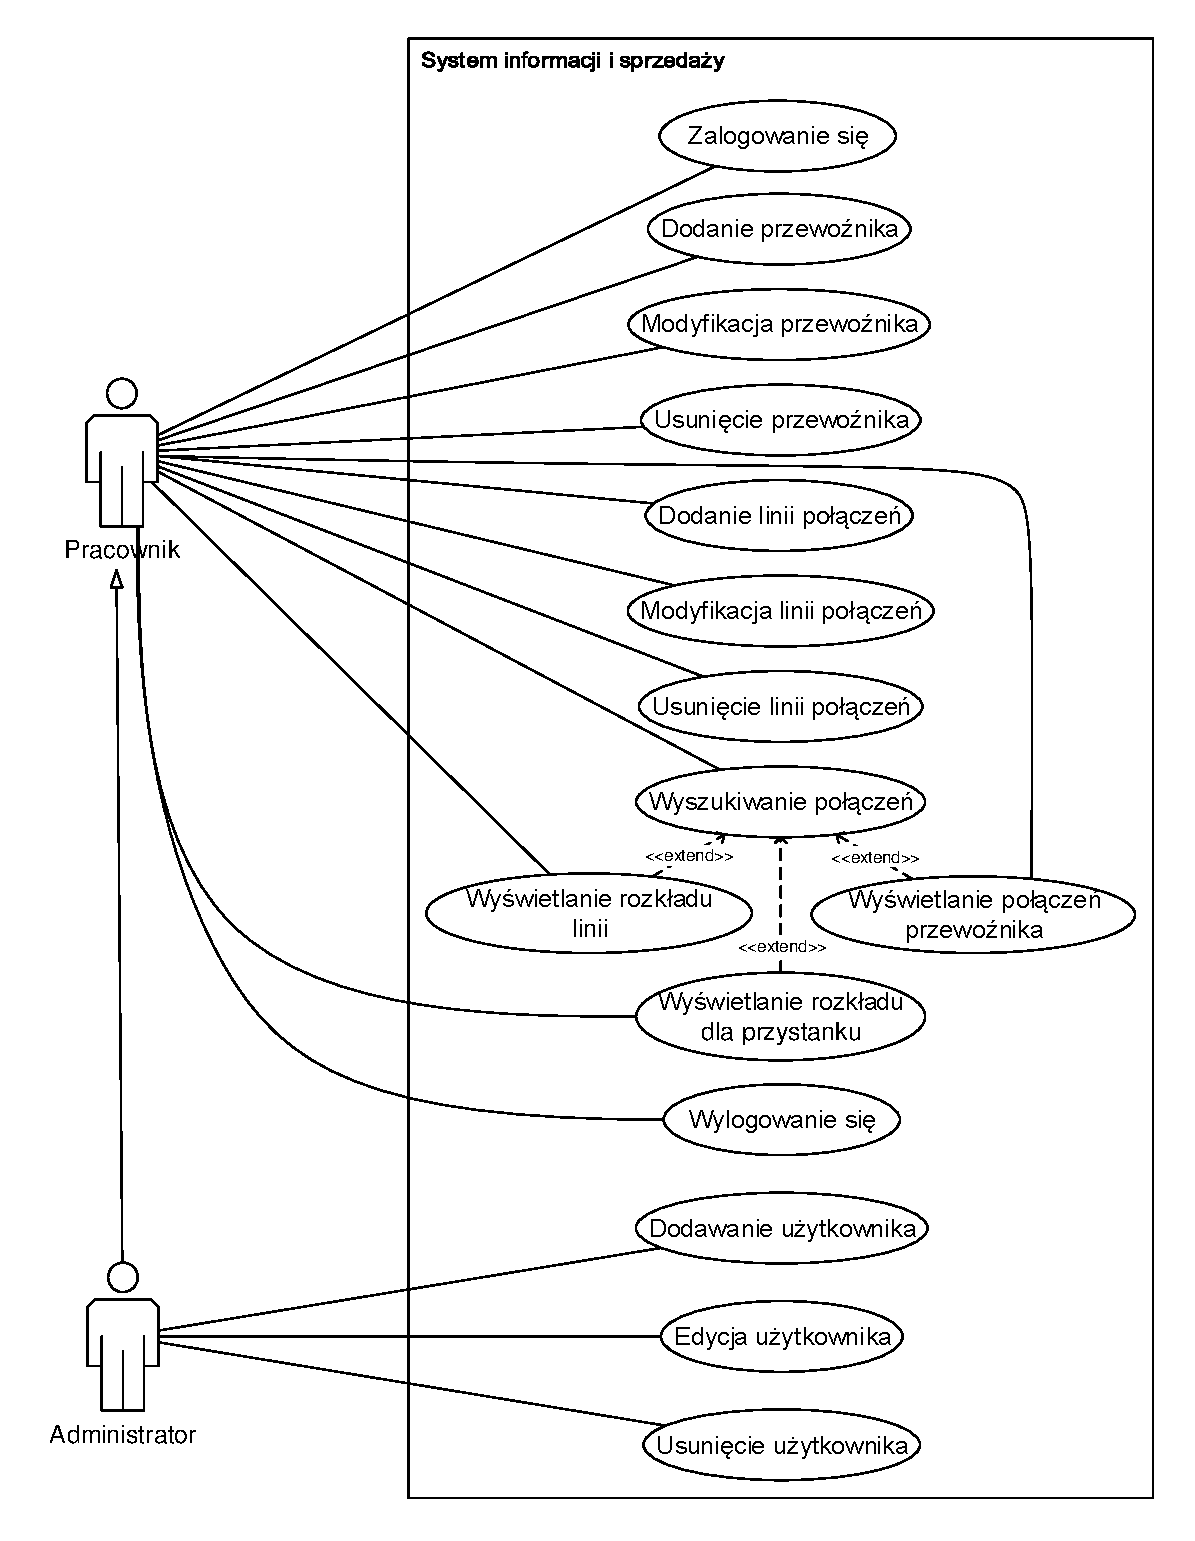
\includegraphics[width=10.5cm]{Resources/PDF/use-case.pdf}
	\caption{Diagram przypadków użycia dla aplikacji}
\end{figure}

\noindent
Poszczególne przypadki są opisane szerzej w poniższej tabeli:
\begin{table}[H]
	\begin{tabularx}{\textwidth}{|c|X|X|X|}
		\hline
		\textbf{Aktor} & \textbf{Nazwa} & \textbf{Opis} & \textbf{Odpowiedź systemu} \\
		\hline
		\multicolumn{4}{|c|}{\textbf{Etap 1}} \\
		\hline
		\multirow{6}{*}{\rotatebox[origin=c]{90}{Administrator}}
		& Dodanie użytkownika
		& Dodanie nowego użytkownika do systemu
		& Potwierdzenie dodania użytkownika \\
		\cline {2-4}
		& Modyfikacja użytkownika
		& Zmiana danych istniejącego użytkownika systemu
		& Potwierdzenie zmodyfikowania rekordu \\
		\cline{2-4}
		& Usunięcie użytkownika
		& Usunięcie konta użytkownika i jego danych z systemu
		& Potwierdzenie usunięcia użytkownika \\
		\hline
		\multirow{26}{*}{\rotatebox[origin=c]{90}{Pracownik}}
		& Zalogowanie się 
		& Zalogowanie się użytkownika do systemu
		& Potwierdzenie zalogowania się lub komunikat o błędzie \\
		\cline{2-4}
		& Wylogowanie się
		& Wylogowanie się pracownika z systemu
		& Potwierdzenie zakończenia pracy z systemem \\
		\cline{2-4}
		& Dodanie przewoźnika
		& Dodanie informacji o nowym przewoźniku do bazy
		& Potwierdzenie dodania danych do bazy \\
		\cline{2-4}
		& Modyfikacja przewoźnika
		& Zmiana danych przewoźnika przechowywanych w bazie
		& Potwierdzenie zmodyfikowania rekordu \\
		\cline{2-4}
		& Usunięcie przewoźnika
		& Usunięcie danych przewoźnika przechowywanych w bazie
		& Potwierdzenie usunięcia rekordu \\
		\cline{2-4}
		& Dodanie linii połączeń
		& Dodanie nowej linii połączeń danego przewoźnika
		& Potwierdzenie dodania linii do bazy \\
		\cline{2-4}
		& Modyfikacja linii połączeń
		& Modyfikacja linii połączeń danego przewoźnika
		& Potwierdzenie modyfikacji rekordu \\
		\cline{2-4}
		& Usunięcie linii połączeń
		& Usunięcie linii połączeń danego przewoźnika
		& Potwierdzenie usunięcia rekordu \\
		\cline{2-4}
		& Wyświetlanie rozkładu linii
		& Wyświetlanie rozkładu jazdy wybranej linii
		& Widok zawierający informacje o przejazdach na wybranej linii \\
		\cline{2-4}
		& Wyświetlanie połączeń przewoźnika
		& Wyświetlanie połączeń obsługiwanych przez danego przewoźnika
		& Widok zawierający informacje o liniach danej firmy \\
		\hline
		\multicolumn{4}{|c|}{\textbf{Etap 2}} \\
		\hline
		\multirow{5}{*}{\rotatebox[origin=c]{90}{Pracownik}}
		& Wyświetlanie rozkładu przystanku
		& Wyświetlanie rozkładu jazdy dla wybranego przystanku
		& Widok zawierający informacje o liniach dla wybranego przystanku \\
		\cline{2-4}
		& Wyszukiwanie połączeń
		& Wyszukiwanie połączeń między wybranymi punktami
		& Widok z listą znalezionych połączeń \\
		\hline
	\end{tabularx}
	\caption{Opisy przypadków użycia dla użytkownika}
\end{table}

\newpage
\subsubsection{Przypadki użycia (interfejs webowy dla klientów)}
Poniższy diagram UML przedstawia przypadki użycia dla internauty korzystającego z aplikacji webowej w celu wyszukiwania połączeń.

\begin{figure}[H]
	\centering
	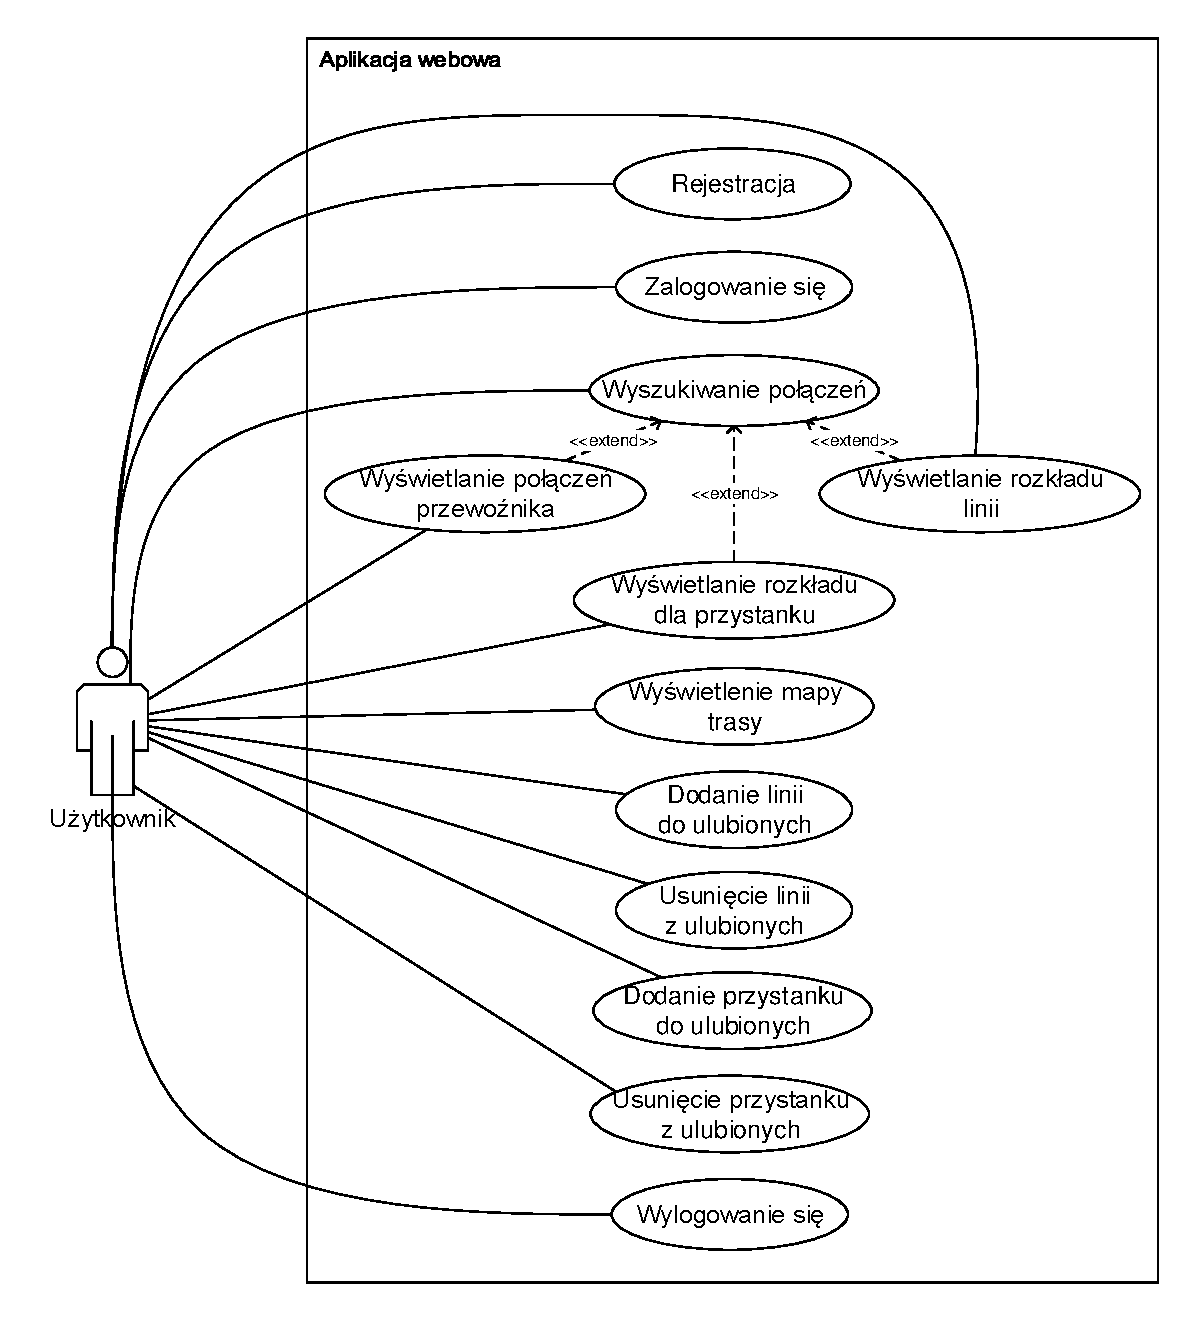
\includegraphics[width=12cm]{Resources/PDF/use-case-web.pdf}
	\caption{Diagram przypadków użycia dla użytkownika aplikacji webowej}
\end{figure}

\newpage
\noindent
Poszczególne przypadki są opisane szerzej w poniższej tabeli:
\begin{table}[H]
	\begin{tabularx}{\textwidth}{|c|X|X|X|}
		\hline
		\textbf{Aktor} & \textbf{Nazwa} & \textbf{Opis} & \textbf{Odpowiedź systemu} \\
		\hline
		\multicolumn{4}{|c|}{\textbf{Etap 3}} \\
		\hline
		\multirow{30}{*}{\rotatebox[origin=c]{90}{Użytkownik}}
		& Rejestracja
		& Utworzenie konta użytkownika w systemie
		& Potwierdzenie utworzenia konta lub komunikat o błędzie \\
		\cline{2-4}
		& Zalogowanie się 
		& Zalogowanie się użytkownika do systemu
		& Potwierdzenie zalogowania się lub komunikat o błędzie \\
		\cline{2-4}
		& Wylogowanie się
		& Wylogowanie się użytkownika z systemu
		& Potwierdzenie wylogowania użytkownika \\
		\cline{2-4}
		& Wyszukiwanie połączeń
		& Wyszukiwanie połączeń między wybranymi punktami
		& Widok z listą znalezionych połączeń \\
		\cline{2-4}
		& Wyświetlanie rozkładu linii
		& Wyświetlanie rozkładu jazdy wybranej linii
		& Widok zawierający informacje o przejazdach na wybranej linii \\
		\cline{2-4}
		& Wyświetlanie rozkładu przystanku
		& Wyświetlanie rozkładu jazdy dla wybranego przystanku
		& Widok zawierający informacje o liniach dla wybranego przystanku \\
		\cline{2-4}
		& Wyświetlanie mapy trasy
		& Wyświetlanie mapy dla wybranej trasy
		& Widok mapy przedstawiające kolejne przystanki na trasie \\
		\cline{2-4}
		& Dodanie linii do ulubionych
		& Dodanie wybranej linii komunikacyjnej do listy ulubionych
		& Potwierdzenie dodania linii do ulubionych \\
		\cline{2-4}
		& Usunięcie linii z ulubionych
		& Usunięcie wybranej linii z listy ulubionych
		& Potwierdzenie usunięcia linii z ulubionych \\
		\cline{2-4}
		& Dodanie przystanku do ulubionych
		& Dodanie wybranego przystanku do listy ulubionych
		& Potwierdzenie dodania przystanku do ulubionych \\
		\cline{2-4}
		& Usunięcie przystanku z ulubionych
		& Usunięcie wybranego przystanku z listy ulubionych
		& Potwierdzenie usunięcia przystanku z ulubionych \\
		\hline
	\end{tabularx}
	\caption{Opisy przypadków użycia dla użytkownika}
\end{table}

\newpage
\subsubsection{User stories}
\begin{enumerate}
	\bfseries
	\item Etap 1
	\begin{enumerate}[label*=\arabic*.]
	\item Interfejs administracyjny dla administratora
		\begin{enumerate}[label*=\arabic*.]
			\mdseries
			\item Jako zalogowany administrator dodaję/modyfikuję użytkownika systemu.\\
				Dowolny zalogowany administrator może dodać nowego użytkowanika lub zmodyfikować informacje o istniejącym użytkowniku, takie jak jego login, hasło oraz uprawnienia.
			\item Jako zalogowany administrator wyszukuję użytkownika. \\
			    Dowolny zalogowany administrator może wyszukać istniejących użytkowników systemu.
		\end{enumerate}
		\item Interfejs administracyjny dla pracownika
		\begin{enumerate}[label*=\arabic*.]
			\mdseries
			\item Jako zalogowany pracownik dodaję/modyfikuję przewoźnika. \\
				Dowolny zalogowany pracownik może dodać nowego przewoźnika lub zmodyfikować informacje o przewoźniku, takie, jak: nazwę i adres firmy, numer REGON oraz jej stronę internetową.
			\item Jako zalogowany pracownik dodaję/modyfikuję linię połączeń. \\
				Dowolny zalogowany pracownik może dodać nowe połączenie lub zmodyfikować informacje o istniejącym połączeniu takie jak: przystanki, czas odjazdu i przyjazdu na poszczególnych przystankach, ilość dostępnych miejsc w danym kursie, podstawowa cena biletu.
			\item Jako zalogowany pracownik wyszukuję połączenie. \\
			    Dowolny zalogowany pracownik może wyszukać dostępne połączenia wybranej linii.
		 	\item Jako zalogowany pracownik wyświetlam rozkład jazdy danej linii. \\
			    Dowolny zalogowany pracownik może wyszukać rozkład jazdy danej linii
			    komunikacyjnej i go wyświetlić.
	    	\item Jako zalogowany pracownik wyświetlam połączenia dla danego przewoźnika. \\
			    Dowolny zalogowany pracownik może wyświetlić połączenia od danego przewoźnika.
		\end{enumerate}
	\end{enumerate}
	\item Etap 2
	\begin{enumerate}[label*=\arabic*.]
		\item Interfejs administracyjny dla pracownika
		\begin{enumerate}[label*=\arabic*.]
			\mdseries
		 	\item Jako zalogowany pracownik wyświetlam rozkład jazdy dla danego przystanku. \\
			    Dowolny zalogowany pracownik może wyświetlić rozkład jazdy dla danego przystanku.
		 	\item Jako zalogowany pracownik wyświetlam połączenia pomiędzy wybranymi punktami. \\
			    Dowolny zalogowany pracownik może wyszukać dostępne bezpośrednie połączenia pomiędzy wybranymi punktami. 
		\end{enumerate}
	\end{enumerate}
	\item Etap 3
	\begin{enumerate}[label*=\arabic*.]
		\item Interfejs webowy
		\begin{enumerate}[label*=\arabic*.]
			\mdseries
		 	\item Jako dowolny użytkownik wyświetlam rozkład jazdy danej linii. \\
			    Dowolny użytkownik (zalogowany lub nie) może wyszukać rozkład jazdy danej linii
			    komunikacyjnej i go wyświetlić.
		 	\item Jako dowolny użytkownik wyświetlam rozkład jazdy dla danego przystanku. \\
			    Dowolny użytkownik (zalogowany lub nie) może wyświetlić rozkład jazdy dla danego przystanku.
		 	\item Jako dowolny użytkownik wyświetlam połączenia pomiędzy wybranymi punktami. \\
			    Dowolny użytkownik (zalogowany lub nie) może wyszukać dostępne bezpośrednie połączenia pomiędzy wybranymi punktami.
		 	\item Jako niezalogowany użytkownik zakładam konto na witrynie. \\
			    Dowolny niezalogowany użytkownik może utworzyć własne konto w aplikacji, specyfikując nazwę swojego konta oraz hasło.
		 	\item Jako zalogowany użytkownik dodaję linię połączeń do ulubionych/usuwam linię z ulubionych. \\
			    Dowolny zalogowany użytkownik może oznaczać dowolną linię połączeń jako ulubioną oraz usuwać ją z listy ulubionych.
		 	\item Jako zalogowany użytkownik dodaję przystanek do ulubionych/usuwam przystanek z ulubionych. \\
			    Dowolny zalogowany użytkownik może oznaczać dowolny przystanek jako ulubiony oraz usuwać go z listy ulubionych.
		\end{enumerate}
	\end{enumerate}
\end{enumerate}

\subsection{Wymagania niefunkcjonalne}
Poniższa tabela zawiera rozpisane wymagania niefunkcjonalne narzucone dla systemu.
\begin{table}[H]
	\begin{tabularx}{\textwidth}{|c|c|c|X|}
		\hline
		\textbf{Obszar wymagań} & \textbf{Nr} & \textbf{Etap} & \textbf{Opis} \\
		\hline
		\multirow{8}{*}{Użyteczność (\textit{Usability})}
		& \multirow{2}{*}{1}
		& \multirow{2}{*}{1}
		& Rozmiar czcionki użytej w aplikacji musi być nie mniejszy niż 12 punktów. \\
		\cline{2-4}
		& \multirow{3}{*}{2}
		& \multirow{3}{*}{1}
		& Aplikacja powinna obsługiwać zmianę rozmiaru okna w sposób który umożliwia korzystanie ze wszystkich jej funkcjonalności (tzw. responsive design). \\
		\cline{2-4}
		& \multirow{3}{*}{3}
		& \multirow{3}{*}{2}
		& Dane wprowadzane przez użytkownika powinny być sprawdzane pod kątem poprawności przed wysyłaniem zapytań do bazy. \\
		\hline
		\multirow{5}{*}{Niezawodność (\textit{Reliability})}
		& \multirow{3}{*}{4}
		& \multirow{3}{*}{1}
		& Aplikacja musi być odporna na dokonywanie jednoczesnych zmian tego samego rekordu bazy przez wielu pracowników jednocześnie. \\
		\cline{2-4}
		& \multirow{2}{*}{5}
		& \multirow{2}{*}{3}
		& Interfejs webowy nie powinien umożliwiać modyfikowania danych w bazie (z wyjątkiem tabel dotyczących kont). \\
		\hline
		\multirow{8}{*}{Wydajność (\textit{Performance})}
		& \multirow{3}{*}{6}
		& \multirow{3}{*}{1}
		& Aplikacja powinna dodawać nowe obiekty do systemu w czasie nie dłuższym niż 1 sekundę, przy 50 żądaniach dodania obiektu na minutę. \\
		\cline{2-4}
		& \multirow{2}{*}{7}
		& \multirow{2}{*}{1}
		& Zużycie pamięci RAM przez aplikację nie powinno przekroczyć 500 megabajtów. \\
		\cline{2-4}
		& \multirow{3}{*}{8}
		& \multirow{3}{*}{1}
		& Wyszukiwanie połączenia między określonymi miastami powinno trwać mniej niż 2 sekundy, przy ok. 10 tys. rekordów. \\
		\hline
		\multirow{2}{*}{Utrzymanie (\textit{Supportability})}
		& \multirow{2}{*}{9}
		& \multirow{2}{*}{1}
		& Do aplikacji dołączona zostanie instrukcja wykonywania kopii zapasowej danych. \\
		\hline
	\end{tabularx}
	\caption{Tabela wymagań niefunkcjonalnych}
\end{table}

\newpage
\subsection{Harmonogram projektu}
Prace przy projekcie będą realizowane według następującego harmonogramu:
\begin{figure}[H]
	\centering
	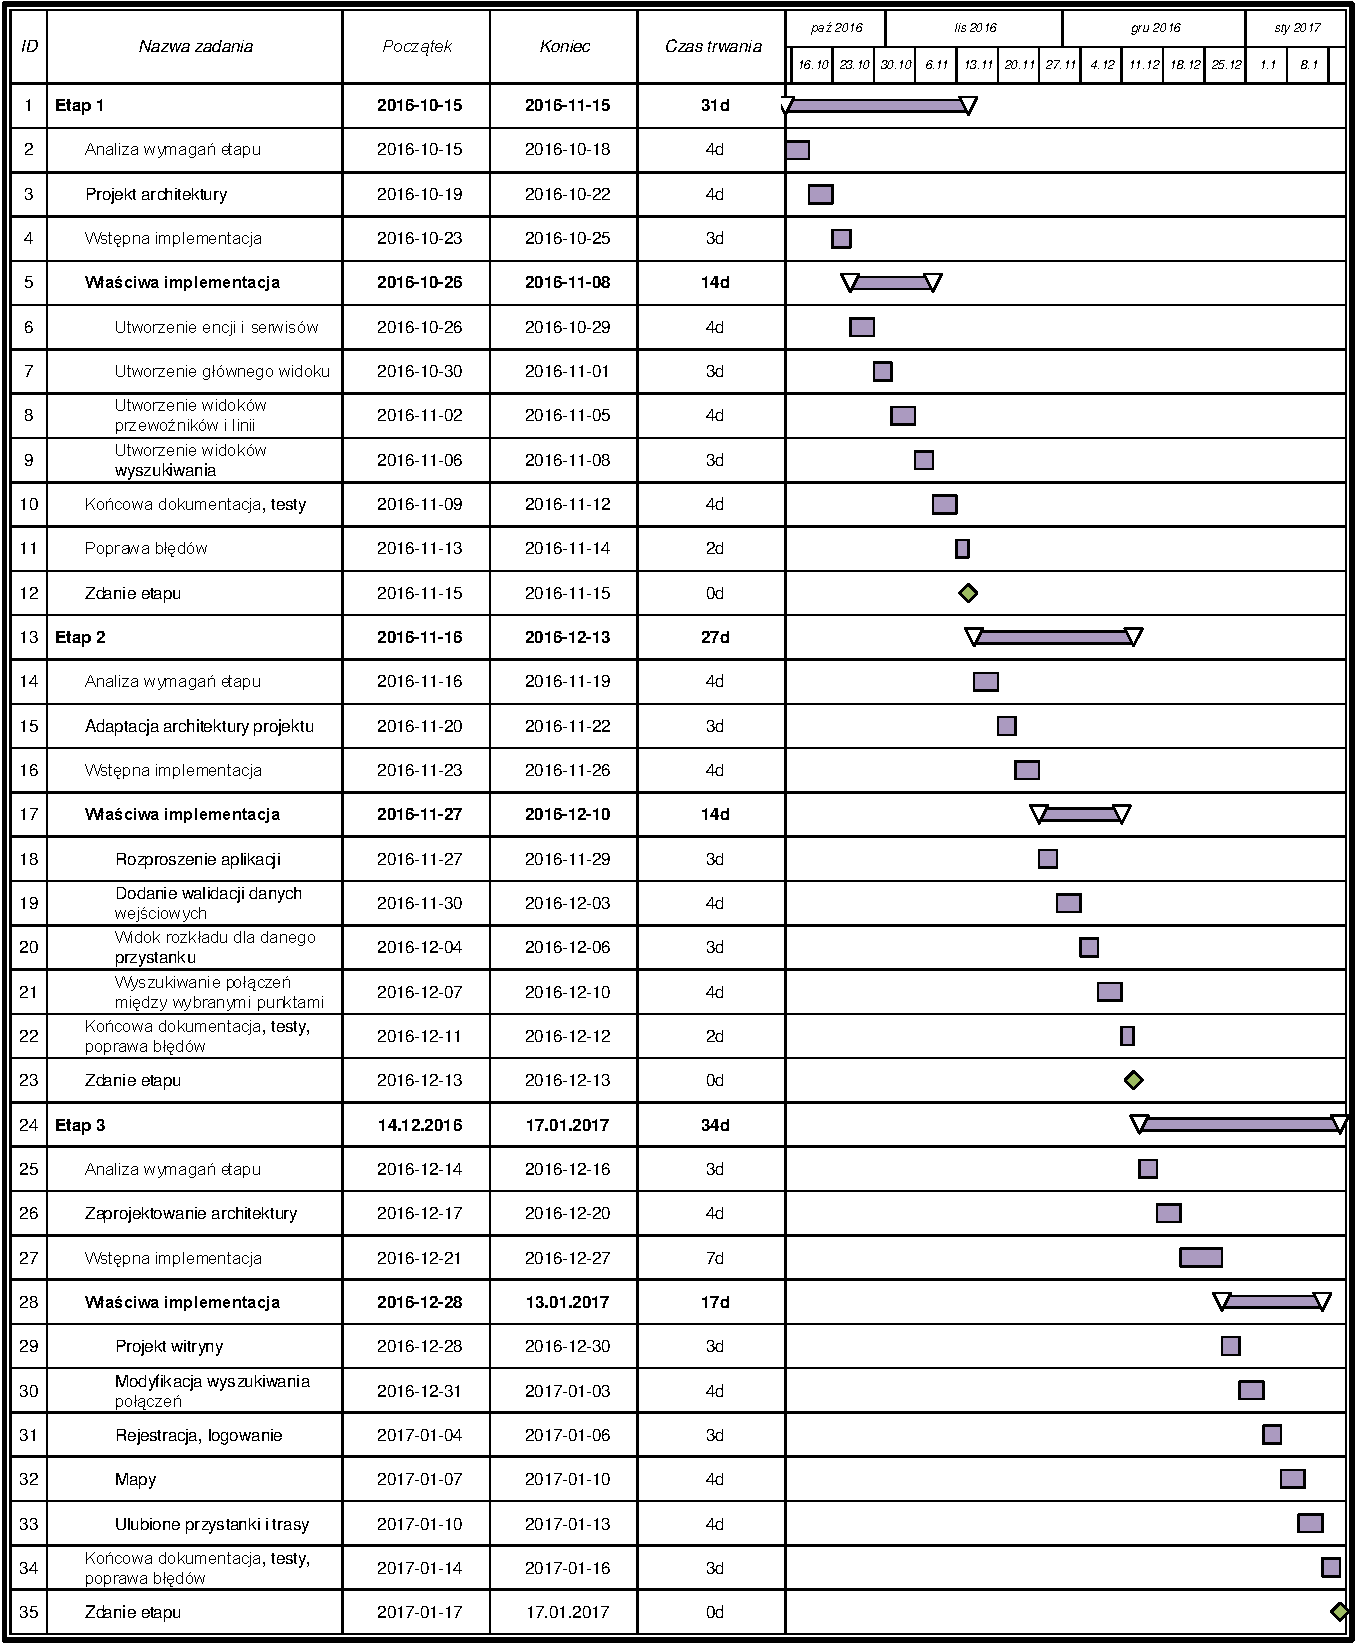
\includegraphics[width=15.5cm]{Resources/PDF/gantt.pdf}
	\caption{Diagram Gantta z planowanym harmonogramem projektu}
\end{figure}

\newpage
\noindent
Kamienie milowe:
\begin{enumerate}
	\bfseries
	\item Etap pierwszy:
	\begin{enumerate}
		\mdseries
		\item 18 października: Zakończenie analizy wymagań funkcjonalnych i niefunkcjonalnych projektu.
		\item 22 października: Zakończenie projektu architektury aplikacji, łącznie z wyróżnieniem komponentów oraz podsystemów.
		\item 25 października: Wstępna implementacja projektu architektury, naniesienie ewentualnych poprawek do architektury wynikających z problemów implementacyjnych.
		\item 29 października: Utworzenie encji biznesowych oraz serwisów wykorzystywanych przez użytkowników.
		\item 1 listopada: Utworzenie głównego widoku aplikacji.
		\item 5 listopada: Utworzenie widoków dodawania przewoźników oraz linii.
		\item 8 listopada: Utworzenie widoków wyszukiwania połączeń oraz wyświetlania połączeń danej linii oraz przewoźnika.
		\item 12 listopada: Zakończenie dokumentacji, testów aplikacji oraz identyfikacji błędów.
		\item 15 listopada: Zakończenie poprawy znalezionych błędów, zdanie projektu łącznie z pełną dokumentacją.
	\end{enumerate}
	\item Drugi etap:
	\begin{enumerate}
		\mdseries
		\item 19 listopada: Zakończenie analizy nowych wymagań funkcjonalnych i niefunkcjonalnych projektu.
		\item 22 listopada: Zakończenie aktualizacji architektury aplikacji, łącznie z wyróżnieniem komponentów oraz podsystemów.
		\item 26 listopada: Wstępna próba rozproszenia aplikacji.
		\item 29 listopada: Wydzielenie serwera aplikacyjnego oraz zintegrowanie go z aplikacją kliencką.
		\item 3 grudnia: Zakończenie implementacji walidacji danych wejściowych.
		\item 6 grudnia: Implementacja rozkładów dla poszczególnych przystanków oraz stworzenie odpowiedniego widoku w aplikacji klienckiej.
		\item 10 grudnia: Dodanie funkcjonalności wyszukiwania połączeń między wybranymi przystankami.
		\item 13 grudnia: Zakończenie poprawy znalezionych błędów, zdanie projektu łącznie z pełną dokumentacją.
	\end{enumerate}
	\item Trzeci etap:
	\begin{enumerate}
		\mdseries
		\item 16 grudnia: Zakończenie analizy nowych wymagań funkcjonalnych i niefunkcjonalnych projektu.
		\item 20 grudnia: Zakończenie aktualizacji architektury aplikacji, łącznie z wyróżnieniem komponentów oraz podsystemów.
		\item 23 grudnia: Wstępna próba wystawienia serwisów WebAPI.
		\item 27 grudnia: Przygotowanie podstawowych widoków w interfejsie webowym.
		\item 30 grudnia: Utworzenie projektu graficznego witryny.
		\item 3 stycznia: Modyfikacja wyszukiwania trasy pomiędzy punktami.
		\item 6 stycznia: Implementacja rejestracji oraz logowania na indywidualne konta użytkowników.
		\item 10 stycznia: Dodanie wyświetlania trasy na mapie.
		\item 13 stycznia: Implementacja funkcjonalności oznaczania tras oraz przystanków jako ulubione.
		\item 17 stycznia: Zakończenie poprawy znalezionych błędów, zdanie projektu łącznie z pełną dokumentacją.
	\end{enumerate}
\end{enumerate}

\subsection{Architektura rozwiązania}
\label{subsec:architecture}
Docelowym środowiskiem aplikacji są małe lub średnie firmy pośredniczące w sprzedaży biletów komunikacyjnych, tzn. przedsiębiorstwa zatrudniające do 250 pracowników, z czego dostęp do systemu miałby dość niski procent tej liczby (w założeniach ok. 20-30\%). Dane, których przechowywanie jest niezbędne do spełnienia wymagań funkcjonalnych mają dość małą zmienność - stosunkowo rzadko ulegają zmianom lub przedawnieniom. Dodatkowo, ze względu na wewnętrzny charakter przechowywanych danych, system powinien być scentralizowany i znajdować się w jednym fizycznym położeniu.
\begin{figure}[H]
	\centering
	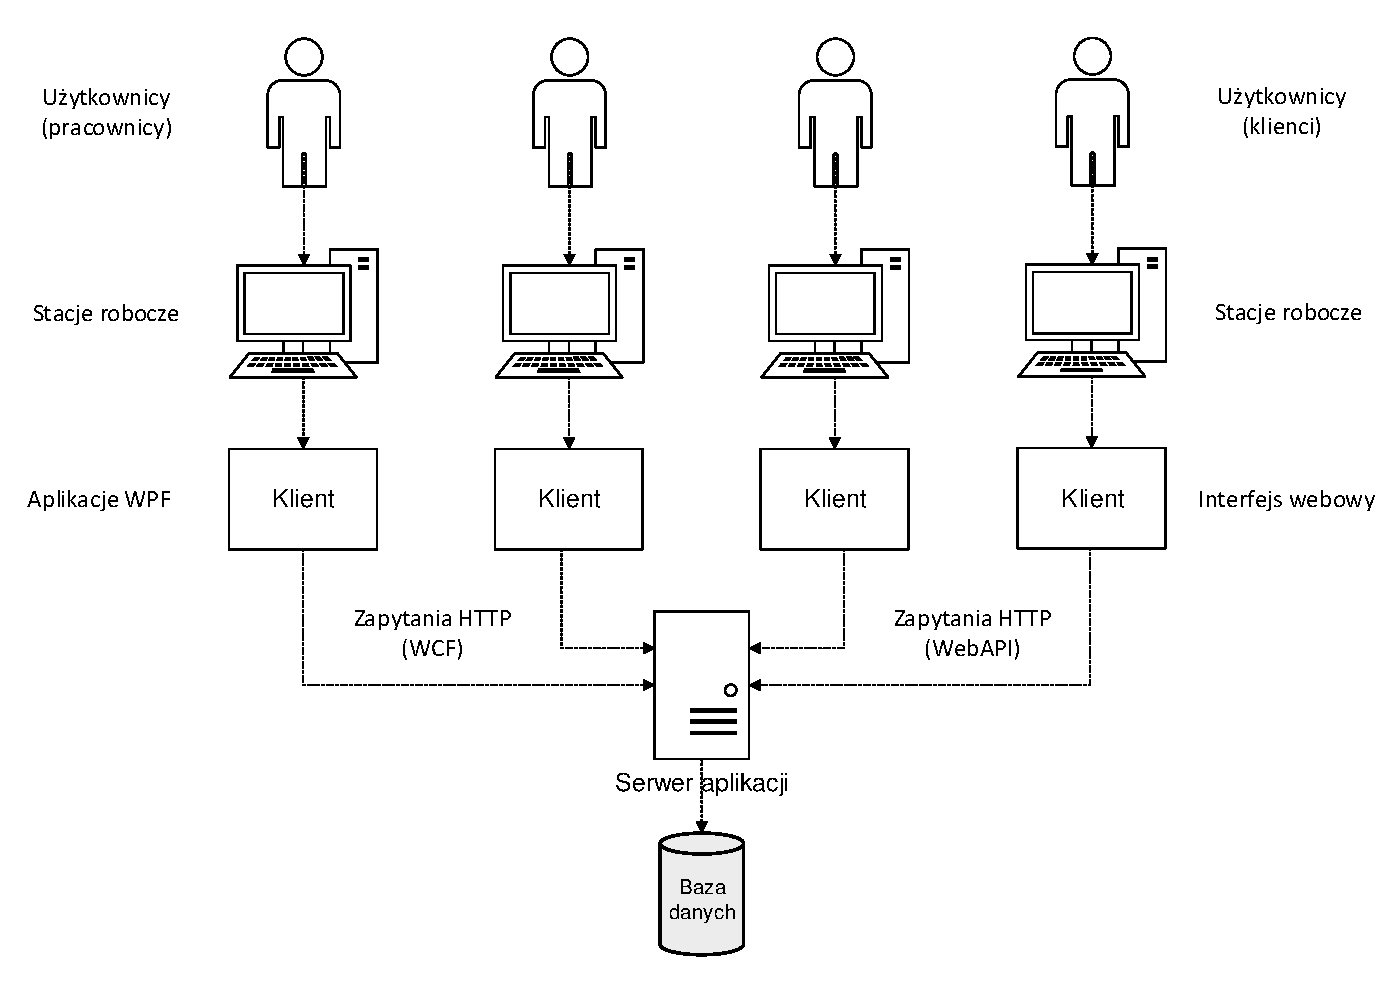
\includegraphics[width=15.5cm]{Resources/PDF/architecture-global.pdf}
	\caption{Schemat architektury systemu}
\end{figure}

\noindent
Biorąc pod uwagę opisany powyżej charakter zamówionego rozwiązania, jako część systemu przeznaczoną dla pracowników wybrany został system rozproszony składający się z aplikacji klienckich typu ,,gruby klient'', instalowanych na stacjach roboczych pracowników oraz administratorów systemu, oraz serwera aplikacyjnego. Dla klientów indywidualnych przygotowano interfejs webowy dostępny z poziomu przeglądarki internetowej.\\[\baselineskip]
Planowana architektura rozwiązania ma charakter warstwowy. W aplikacji przeznaczonej dla pracowników wyróżnione zostały następujące warstwy:
\begin{itemize}
	\item warstwa dostępu do danych - odpowiedzialna za kontakt z bazą oraz odczyt i zapis przechowywanych tam danych,
	\item warstwa biznesowa - odpowiedzialna za wykonywanie poszczególnych usług (np. dodania czy modyfikacji przewoźnika),
	\item warstwa prezentacji - odpowiedzialna za wyświetlanie interfejsu użytkownika.
\end{itemize}
Część przeznaczona dla internautów może być opisana następującymi warstawami:
\begin{itemize}
	\item warstwa dostępu do danych - odpowiedzialna za kontakt z bazą,
	\item warstwa biznesowa - odpowiedzialna za wykonywanie poszczególnych usług (np. wyszukanie trasy przejazdu),
	\item warstwa prezentacji - odpowiedzialna za wyświetlanie interfejsu webowego.
\end{itemize}
Głównymi powodami zaproponowania architektury warstwowej były:
\begin{itemize}
	\item możliwość wymiany silnika bazodanowego oraz warstwy prezentacji bez naruszania warstwy biznesowej,
	\item podział odpowiedzialności na poszczególne warstwy,
	\item spójny charakter wymagań - podział na podsystemy jest zbędny.
\end{itemize}
Ze względu na małą liczbę użytkowników niska skalowalność oraz wydajność rozwiązań warstwowych zostały uznane za ryzyko drugorzędne.

\subsubsection{Serwer aplikacyjny}
Serwer aplikacyjny to pojedyncza stacja robocza w sieci wewnętrznej, odpowiadająca za obsługę i odpowiedź na zapytania kierowane do niego przez aplikacje klienckie różnej postaci. Serwer udostępnia wszystkim klientom usługi, w których określone są typy danych wyjściowych i wejściowych. Komunikacja z klientami odbywa się za pomocą protokołu HTTP.

\subsubsection{Aplikacja kliencka (dla pracowników)}
\begin{figure}[H]
	\centering
	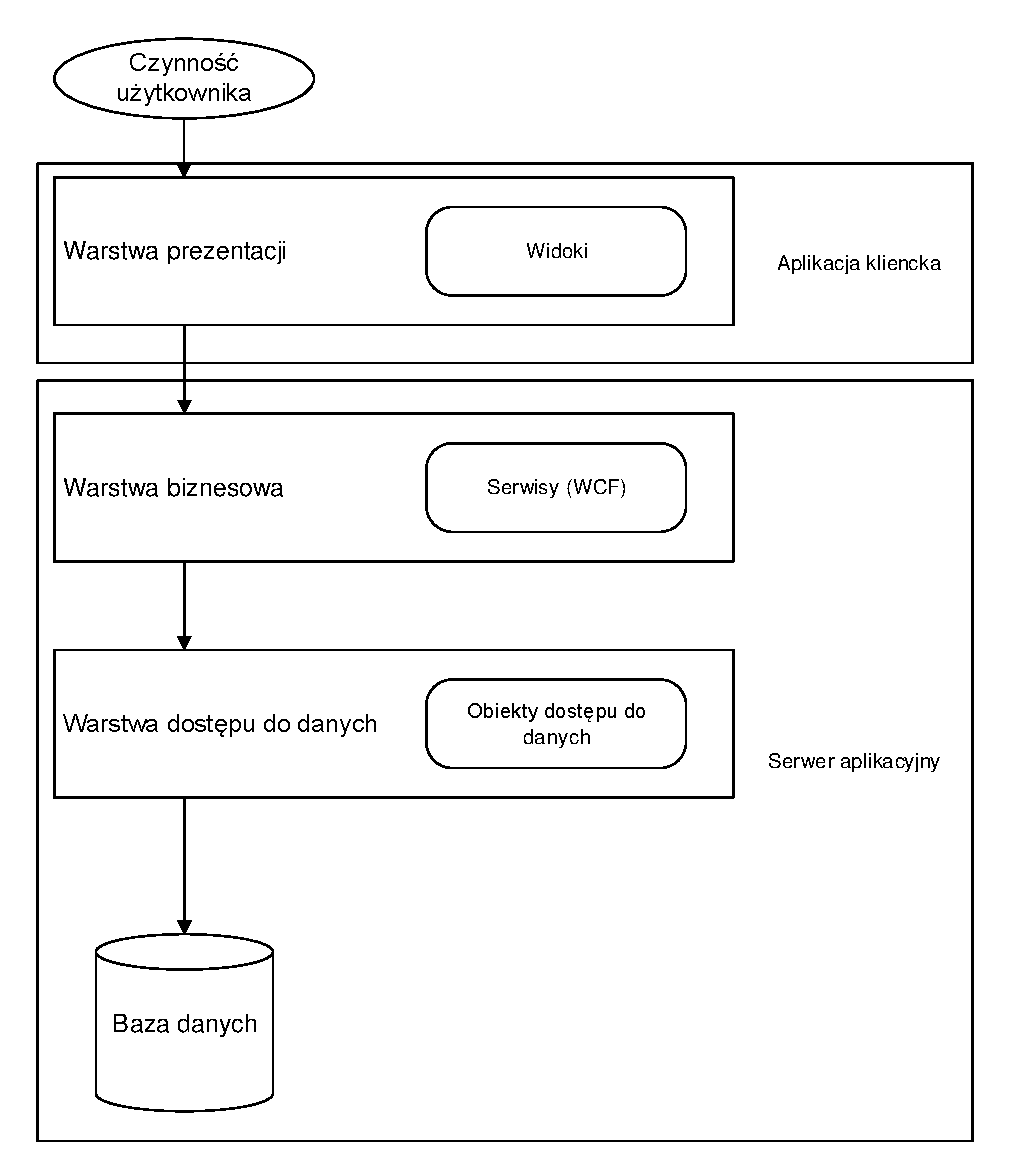
\includegraphics[width=10cm]{Resources/PDF/architecture-fat-client.pdf}
	\caption{Schemat wykonywania czynności pracownika}
\end{figure}
Aplikacje klienckie mają postać ,,grubego klienta'', instalowanego na stacjach roboczych konkretnych użytkowników. Wykonywanie wszystkich żądań użytkownika delegowane jest do serwera aplikacyjnego za pośrednictwem udostępnionych usług; odpowiedzią jest informacja o powodzeniu, lub błąd wykonania. W aplikacji klienckiej nie znajdują się elementy związane z logiką biznesową.

\subsubsection{Interfejs webowy}
\begin{figure}[H]
	\centering
	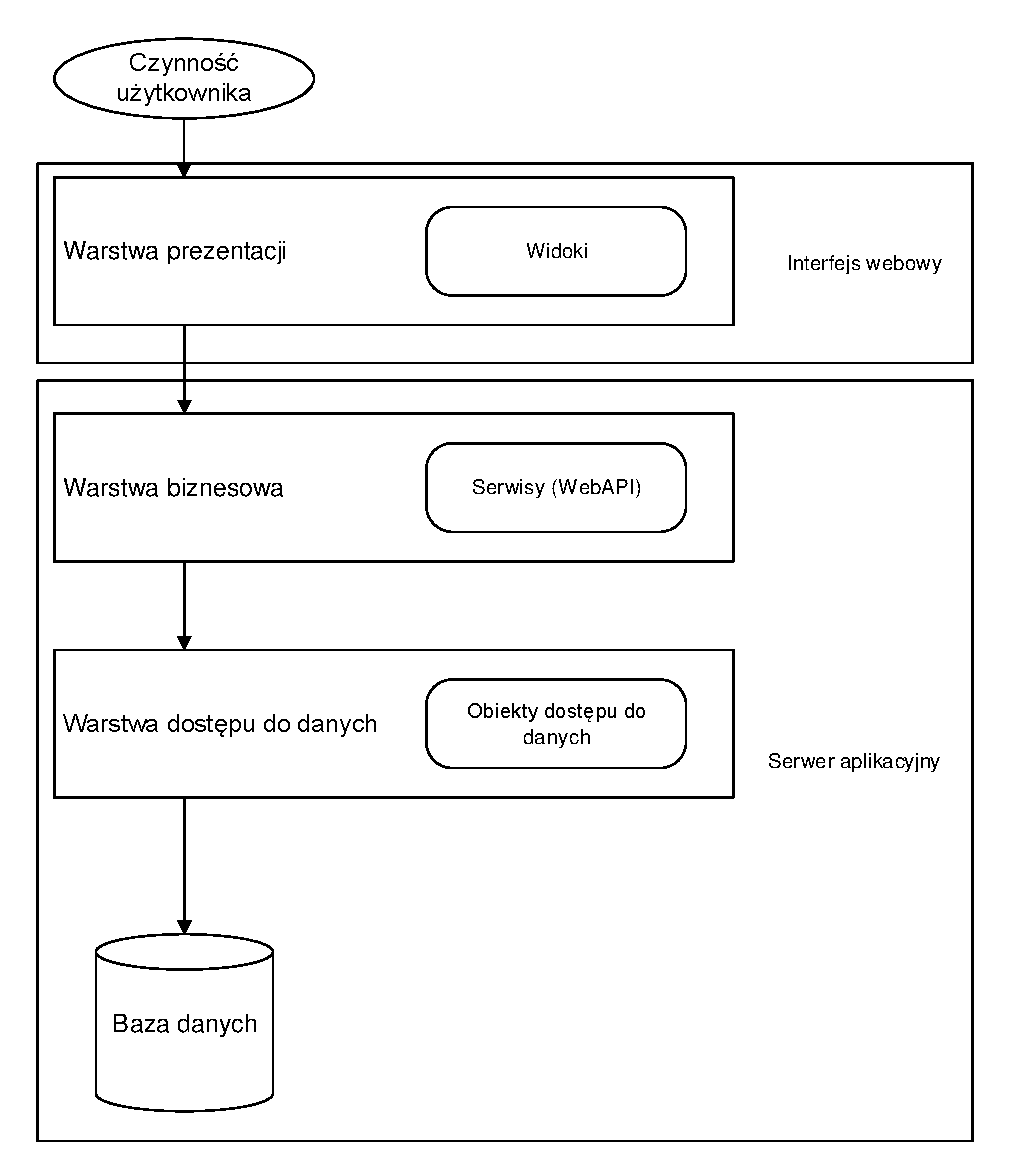
\includegraphics[width=10cm]{Resources/PDF/architecture-web-client.pdf}
	\caption{Schemat wykonywania czynności klienta}
\end{figure}
Interfejs webowy umożliwia użytkownikom wysyłanie zapytań do serwera aplikacyjnego z poziomu przeglądarki internetowej. Podobnie jak w przypadku aplikacji klienckiej, nie ma tutaj logiki biznesowej.

\newpage
\section{Dokumentacja końcowa (powykonawcza)}

\subsection{Wymagania systemowe}
Aby zapewnić poprawne działanie aplikacji klienckiej, wymagane są następujące komponenty:
\begin{enumerate}
	\item System operacyjny Windows 7 lub nowszy.
	\item .NET Framework 4.5.2 lub nowszy.
\end{enumerate}
Aby zapewnić poprawne działanie serwera aplikacyjnego, wymagane są następujące komponenty:
\begin{enumerate}
	\item System operacyjny Windows Server 2008 lub nowszy.
	\item .NET Framework 4.5.2 lub nowszy.
	\item MS SQL Server 2014 lub nowszy.
\end{enumerate}

\subsection{Biblioteki wraz z określeniem licencji}
W budowie aplikacji zostały użyte następujące biblioteki oraz komponenty firm trzecich:

\begin{table}[H]
	\begin{tabularx}{\textwidth}{|r|l|X|l|c|}
		\hline
		\textbf{Nr} & \textbf{Komponent i wersja} & \textbf{Opis} & \textbf{Licencja} & \\
		\hline
		1 & 
		Castle.Core, 3.3.3 &
		Wykorzystywana do tworzenia obiektów \textit{proxy}. Zależność biblioteki Moq. &
		Apache License 2.0 &
		\cite{castlecore} \\
		\hline
		2 &
		Entity Framework, 6.1.3 &
		Framework do mapowania obiektowo-relacyjnego (ORM). &
		Apache License 2.0 &
		\cite{entityframework} \\
		\hline
		3 &
		FluentAssertions, 4.17.0 &
		Wykorzystywany w testach jednostkowych w celu ułatwienia pisania asercji. &
		Apache License 2.0 &
		\cite{fluentassertions} \\
		\hline
		4 &
		Moq, 4.5.28 &
		Używany w testach jednostkowych do tworzenia obiektów zastępczych (tzw. \emph{mock object}). &
		\mbox{\hyperref[abbr:bsd]{BSD}} 3-Clause &
		\cite{moq} \\
		\hline
		5 &
		NUnit, 3.5.0 &
		Framework do wykonywania testów jednostkowych. &
		\mbox{\hyperref[abbr:mit]{MIT}} &
		\cite{nunit} \\
		\hline
		6 &
		ReactiveUI, 6.5.2 &
		Biblioteka wspomagająca w realizacji wzorca \hyperref[abbr:mvvm]{MVVM} w aplikacji klienckiej, zintegrowana z Reactive Extensions. &
		\mbox{\hyperref[abbr:mspl]{MS-PL}} &
		\cite{reactiveui} \\
		\hline
		7 &
		Reactive Extensions, 2.2.5 &
		Biblioteka wspomagająca w programowaniu aplikacji opartych na asynchronicznym przetwarzaniu danych oraz zdarzeniach. Zależność ReactiveUI. &
		Apache License 2.0 &
		\cite{reactiveextensions} \\
		\hline
		8 &
		Splat, 1.4.0 &
		Kontener \hyperref[abbr:ioc]{IoC} wspomagający w realizacji wzorca wstrzykiwania zależności. &
		\mbox{\hyperref[abbr:mit]{MIT}} &
		\cite{splat} \\
		\hline
		9 &
		MahApps.Metro, 1.3.0 &
		Biblioteka zawierająca kontrolki interfejsu użytkownika. &
		\mbox{\hyperref[abbr:mspl]{MS-PL}} &
		\cite{mahapps} \\
		\hline
		10 &
		AngularJS, 1.5.9 &
		Framework wspomagający tworzenie i rozwijanie Single Page Application. &
		\mbox{\hyperref[abbr:mit]{MIT}} &
		\cite{angularjs} \\
		\hline
		11 &
		Angular Spinner, 1.5.9 &
		Dyrektywa pokazująca animowany spinner ładowania. &
		\mbox{\hyperref[abbr:mit]{MIT}} &
		\cite{angularspinner} \\
		\hline
		12 &
		Spin.js, 2.3.2.1 &
		Biblioteka definiująca animowany spinner ładowania. &
		\mbox{\hyperref[abbr:mit]{MIT}} &
		\cite{spinjs} \\
		\hline
	\end{tabularx}
\end{table}
\begin{table}[H]
	\begin{tabularx}{\textwidth}{|r|l|X|l|c|}
		\hline
		13 &
		Angular toastr, 2.1.1 &
		Biblioteka pokazująca powiadomienia. &
		\mbox{\hyperref[abbr:mit]{MIT}} &
		\cite{toastr} \\
		\hline
		14 &
		Angular event aggregator, 1.0.0 &
		Biblioteka zawierająca implementację agregatora eventów. &
		\mbox{\hyperref[abbr:mit]{MIT}} &
		\cite{angularevent} \\
		\hline
		15 &
		Angular UI Router, 0.3.1 &
		Biblioteka wspomagająca nawigację na stronie. &
		\mbox{\hyperref[abbr:mit]{MIT}} &
		\cite{uirouter} \\
		\hline
		16 &
		Angular UI Bootstrap, 2.3.2 &
		Biblioteka dyrektyw dla Bootstrapa. &
		\mbox{\hyperref[abbr:mit]{MIT}} &
		\cite{uibootstrap} \\
		\hline
		17 &
		Font Awesome, 4.7.0 &
		Biblioteka czcionek i ikonek. &
		Open Font License 1.1 &
		\cite{fontawesome} \\
		\hline
		18 &
		Bootstrap, 3.3.7 &
		Framework CSS. &
		\mbox{\hyperref[abbr:mit]{MIT}} &
		\cite{bootstrap} \\
		\hline
		19 &
		OAuth 2.0, 3.0.1 &
		Protokół zabezpieczający API. &
		Apache License 2.0 &
		\cite{oauth} \\
		\hline
		20 &
		Unity, 4.0.1 &
		Kontener dependency injection. &
		\mbox{\hyperref[abbr:mspl]{MS-PL}} &
		\cite{unity} \\
		\hline
		21 &
		AngularJS Google Maps, 1.17.0 &
		Dyrektywa wspierająca mapy Google. &
		\mbox{\hyperref[abbr:mit]{MIT}} &
		\cite{ngmap} \\
		\hline
		22 &
		jQuery, 3.1.1 &
		Biblioteka ułatwiająca korzystanie z JavaScriptu. &
		\mbox{\hyperref[abbr:mit]{MIT}} &
		\cite{jquery} \\
		\hline
	\end{tabularx}
	\caption{Lista użytych bibliotek i komponentów}
\end{table}

\subsection{Instrukcja instalacji}
Aby zainstalować aplikację na serwerze aplikacyjnym, należy wykonać następujące kroki:
\begin{enumerate}
	\item Zainstalowanie \textbf{.NET Framework w wersji 4.0 lub późniejszej}, usług \textbf{Internet Information Service w wersji 8 lub późniejszej}, \textbf{Microsoft SQL Server w wersji 2014 lub późniejszej} oraz \textbf{ASP.NET} na serwerze aplikacyjnym. \\
	Aplikacja do funkcjonowania wymaga instalacji serwera bazy danych Microsoft SQL Server w wersji 2014 lub późniejszej. Instrukcję instalacji SQL Server można znaleźć w pozycji bibliografii \cite{sqlserver}. Instrukcję instalacji usługi IIS można znaleźć w pozycji \cite{iis}. Instrukcję konfiguracji usługi ASP.NET można znaleźć w pozycji \cite{aspnet}.
	\item \textbf{Instalacja serwisów WCF, kontrolerów API oraz Web na serwerze aplikacyjnym} \\
	Po skopiowaniu plików dostarczonych jako część aplikacji do wybranej lokalizacji na serwerze, należy otworzyć aplikację \textbf{IIS Manager}. Tworzymy nową stronę w zakładce \textbf{Sites} po lewej, po czym klikamy \textbf{View Applications} po prawej stronie. Następnie z prawej strony wybieramy \textbf{Add Application}. W okienku wpisujemy \textbf{Alias}, który będzie służyć jako prefiks endpointów oraz podajemy ścieżkę do plików serwisowych aplikacji. Proces dodawania strony internetowej powtarzamy dla każdej strony, którą chcemy później uruchomić (WCF, API, Web).
	\begin{itemize}
		\item \textbf{Uwaga:} Serwisy WCF powinny zostać zainstalowane na osobnym serwerze, zaś API oraz witryna Web -- na innym. Serwer obsługujący serwisy WCF powinien być odseparowany od publicznego Internetu. Szczegółowe informacje znajdują się w sekcji \ref{subsec:architecture}.
	\end{itemize}
	\item \textbf{Konfiguracja connection stringów} \\
	Po dodaniu aplikacji należy kliknąć na nią po lewej stronie w okienku \textbf{Connections}, następnie na \textbf{Connection strings} i wyedytować connection string, aby wskazywał on na zainstalowaną instancję bazy.
	\item \textbf{Konfiguracja API URL i Google Maps Token} \\
	W pliku \textbf{app.config.js} znajduje się adres dostępu do API pod zmienną \textbf{baseApiUrl} oraz token konieczny do korzystania z Google Maps pod zmienną \textbf{googleMapsToken}. Należy je odpowiednio uzupełnić przed uruchomieniem strony.
	\item \textbf{Uruchomienie serwera} \\
	Przed pierwszym uruchomieniem aplikacji należy upewnić się, że serwer działa, uruchamiając \textbf{SQL Server Configuration Manager} i sprawdzając, czy status usługi \textbf{MSSQLSERVER} to \textbf{Running}.
	\item \textbf{Pierwsze uruchomienie grubego klienta} \\
	Po uruchomieniu aplikacji należy wpisać dowolne dane logowania i wcisnąć przycisk \textbf{Login}. W tym momencie przycisk powinien się zablokować, a po kilkunastu sekundach powinien pojawić się komunikat o błędnych danych logowania. Oznacza to, że schemat bazy danych został pomyślnie utworzony; aby to potwierdzić, należy uruchomić \textbf{SQL Server Management Studio} i zweryfikować, że schemat bazy danych został utworzony.
	\item \textbf{Wykonanie skryptu z przykładowymi danymi} \\
	Po wykonaniu poprzedniego kroku, należy za pośrednictwem \textbf{SQL Server Management Studio} wykonać dostarczony skrypt T-SQL, aby dodać do bazy danych przykładowe dane. Wówczas można zalogować się do aplikacji używając danych wyspecyfikowanych w poniższej sekcji, a następnie dokonywać dalszego dostosowywania systemu do własnych potrzeb.
\end{enumerate}

\subsection{Instrukcja uruchomienia}
Na serwerze aplikacyjnym należy upenić się, że usługa IIS dla naszej strony oraz instancja serwera MS SQL jest uruchomiona. 
\begin{enumerate}
	\item Otwórz \textbf{SQL Server Configuration Manager} i spradź, czy status usługi (\textbf{MSSQLSERVER}) to \textbf{Running}. Jeżeli nie, uruchom usługę za pomocą przycisku \textbf{Start Service} na pasku pod menu.
	\item Otwórz konsolę \textbf{IIS}.
	\item Wybierz swoją stronę po lewej stronie okna.
	\item Po prawej stronie okna wybierz opcję \textbf{Start}, jeżeli usługa nie jest uruchomiona.
	\item Powtórz punkty 3. i 4. dla wszystkich stron, które chcesz uruchomić (WCF, API, Web).
\end{enumerate}
Na stacji roboczej możemy wówczas uruchomić aplikację, aby połączyć się z serwerem aplikacyjnym.
\begin{enumerate}
	\item Klikamy dwukrotnie plik wykonywalny \textbf{PublicTransport.exe}, aby uruchomić aplikację.
\end{enumerate}
Po uruchomieniu stron API oraz Web, można korzystać z interfejsu webowego, wchodząc na odpowiedni adres w przeglądarce internetowej.

\subsection{Instrukcja użycia}

\subsubsection{Aplikacja dla pracowników}

\paragraph{Logowanie do systemu}
Po uruchomieniu aplikacji przez użytkownika pojawia się okno logowania. Predefiniowane są następujące konta użytkowników:
\begin{itemize}
	\item użytkownik \texttt{root}, hasło \texttt{root}: konto z uprawnieniami administratora,
	\item użytkownik \texttt{employee}, hasło \texttt{password}: konto z uprawnieniami użytkownika,
	\item użytkownik \texttt{guest}, hasło \texttt{guest}: konto bez nadanych uprawnień.
\end{itemize}
\begin{figure}[H]
	\centering
	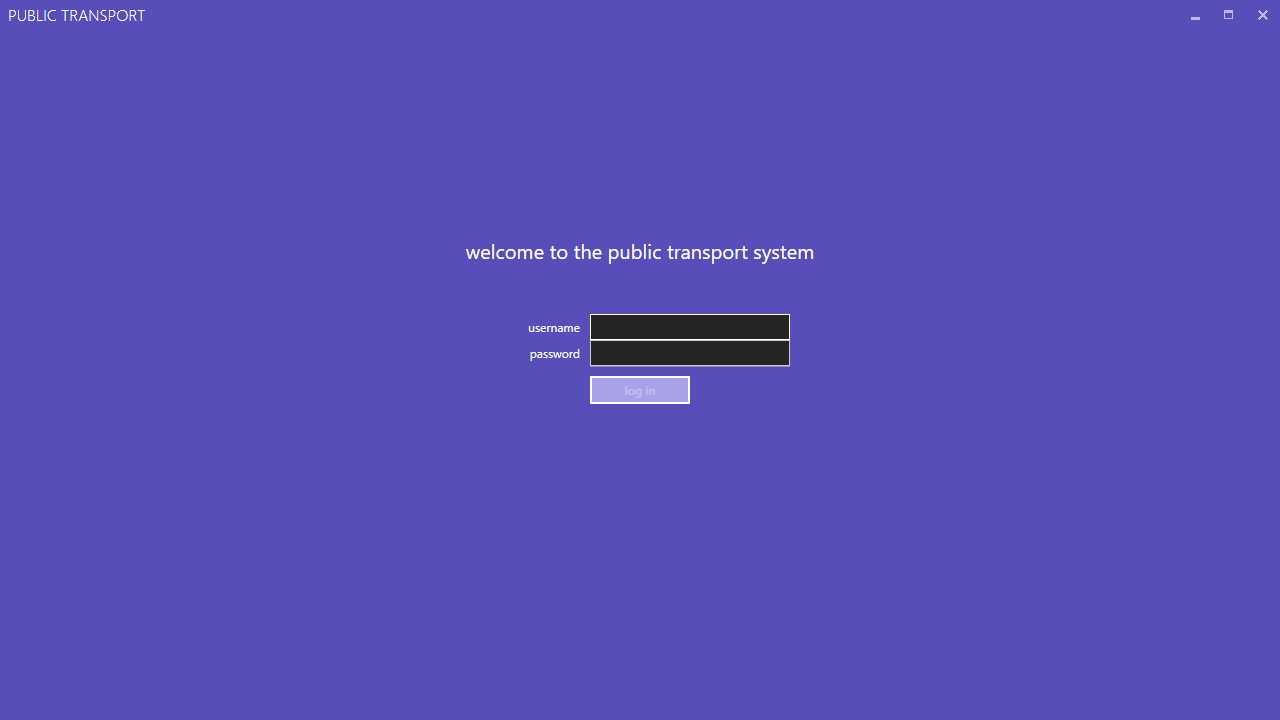
\includegraphics[width=15cm]{Resources/Images/01_login_screen.png}
	\caption{Okno logowania do systemu}
\end{figure}

\paragraph{Główne okno aplikacji}
Po podaniu prawidłowej kombinacji nazwy użytkownika i hasła, wyświetlony zostaje główne okno aplikacji. Po lewej stronie znajduje się menu nawigacyjne, które umożliwia dostęp do poszczególnych części systemu, zaś pod menu znajduje się zaś przycisk odpowiadający za wylogowanie użytkownika z systemu.
\begin{figure}[H]
	\centering
	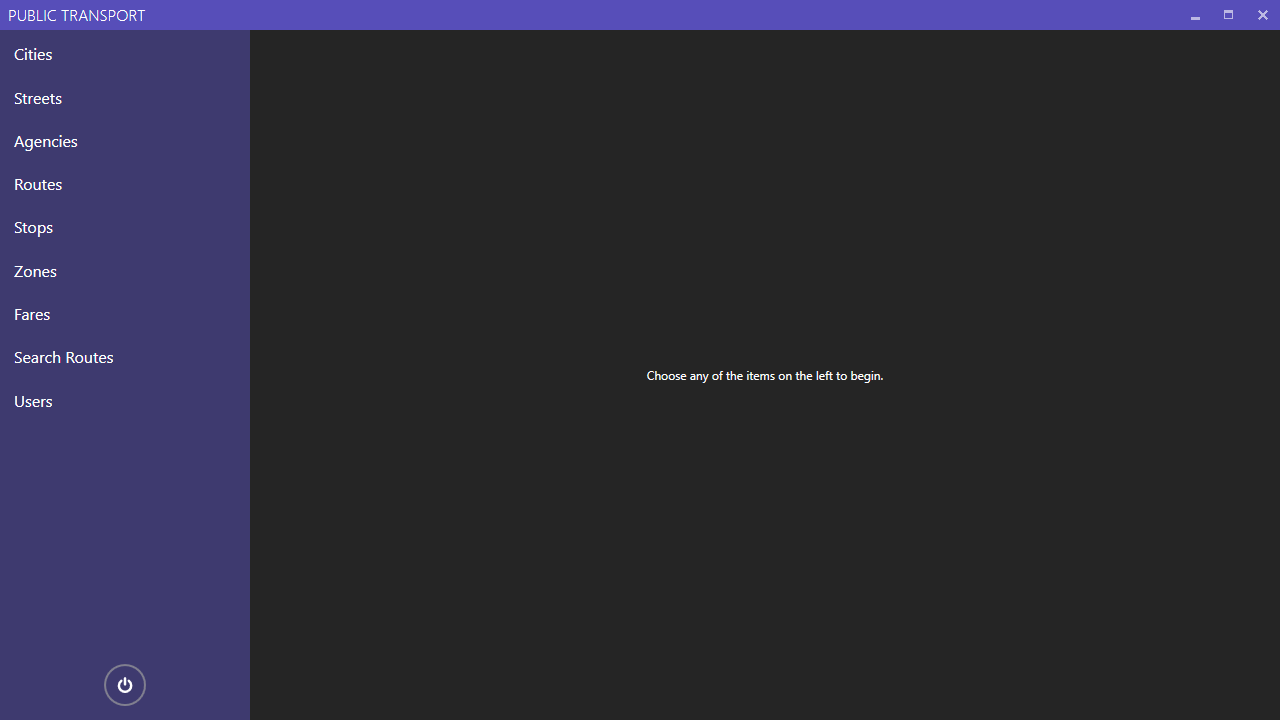
\includegraphics[width=15cm]{Resources/Images/02_main_window.png}
	\caption{Główny widok aplikacji}
\end{figure}
Po kliknięciu dowolnej opcji menu, po prawej stronie aplikacji wyświetla się formularz wyszukiwania odpowiadający wybranej opcji. Dostępne opcje to:
\begin{itemize}
	\item \textbf{Cities}, \textbf{Streets} -- łączy funkcjonalności związane z miastami i ulicami,
	\item \textbf{Agencies} -- agreguje informacje dotyczące przewoźników,
	\item \textbf{Routes} -- wyświetla dane o trasach i przejazdach,
	\item \textbf{Stops} -- pozwala wyszukiwać, edytować i dodawać przystanki,
	\item \textbf{Zones} -- umożliwia wyznaczanie stref taryfowych, na podstawie których obliczana będzie cena biletu,
	\item \textbf{Fares} -- zbiera dane dotyczące taryf przejazdowych i cen biletów,
	\item \textbf{Users} -- zawiera informacje o użytkownikach; widok ten dostępny jest tylko dla administratorów.
\end{itemize}

\paragraph{Wyszukiwanie}
W przypadku wszystkich wyżej wymienionych opcji, po wybraniu po prawej stronie pokazuje się widok pozwalający na przeszukiwanie danych zawartych w bazie dotyczących wybranej zakładki.
\begin{figure}[H]
	\centering
	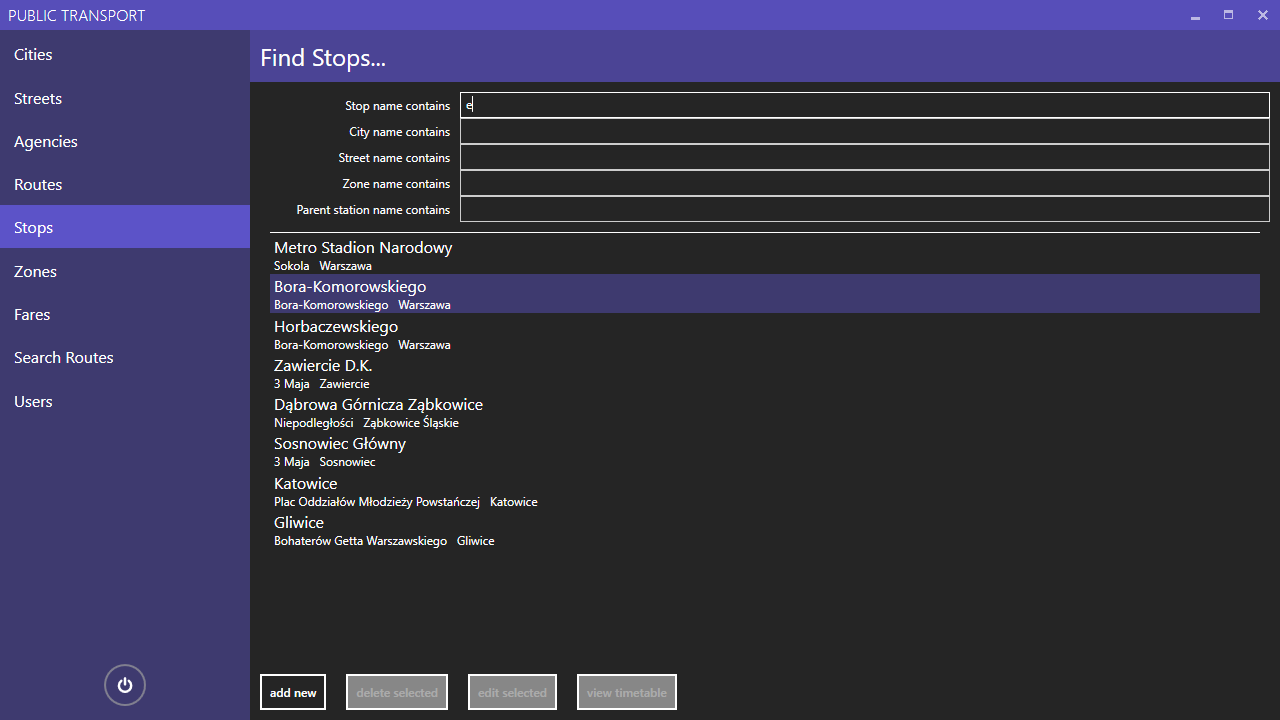
\includegraphics[width=15cm]{Resources/Images/13_filter_stops.png}
	\caption{Przykładowy widok wyszukiwania}
\end{figure}
Po wybraniu opcji lista znalezionych rekordów w bazie będzie pusta. Aby rozpocząć wyszukiwanie, należy zacząć wprowadzanie kryteriów wyszukiwania w polach znajdujących się nad listą. Zawartość listy zaktualizuje się automatycznie w ciągu pół sekundy od zakończenia wprowadzania danych.

Poniżej listy umieszczony jest pasek narzędziowy, umożliwiający dodanie nowego rekordu (\textbf{Add New}) oraz edycję (\textbf{Edit Selected}) bądź usunięcie (\textbf{Delete Selected}) obecnie zaznaczonego rekordu. Pierwszy z tych przycisków jest aktywny zawsze, zaś pozostałe uaktywniają się, gdy zaznaczony jest jeden z elementów listy z wynikami wyszukiwania.

\paragraph{Edycja}
Po wybraniu opcji dodania lub edycji rekordu, po prawej stronie wyświetli się formularz umożliwiający na wprowadzenie danych nowego rekordu.
\begin{figure}[H]
	\centering
	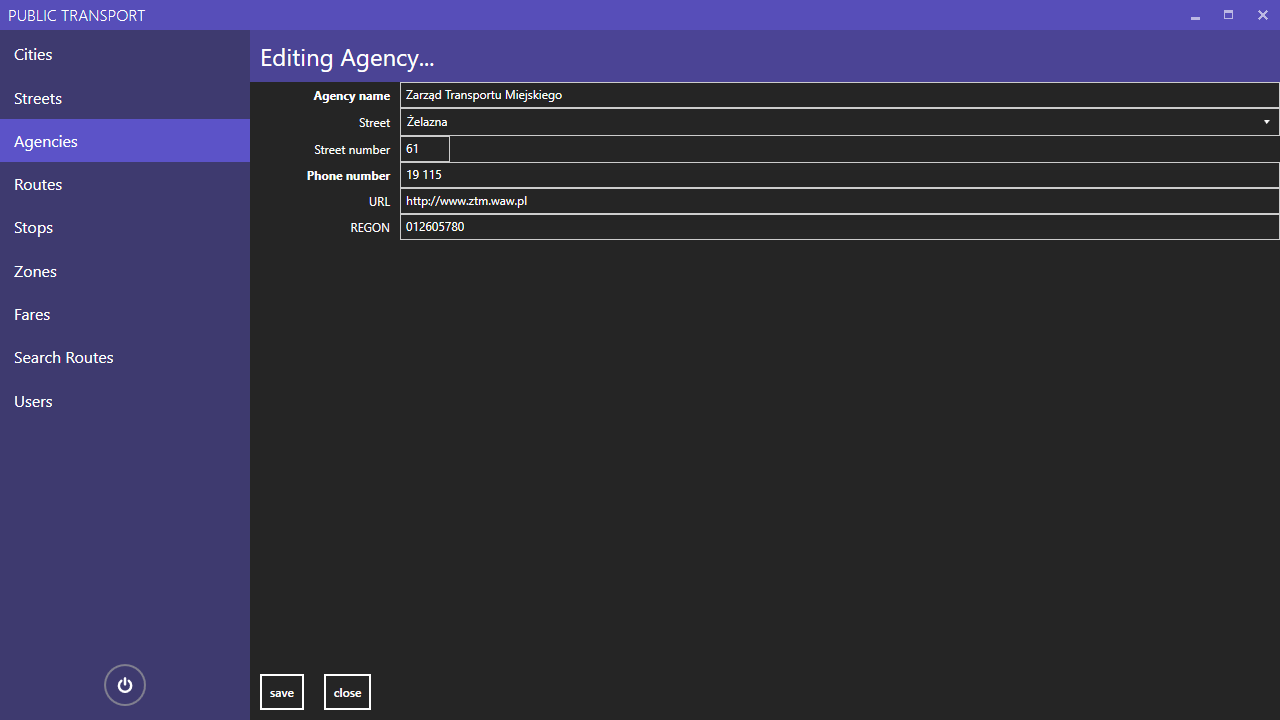
\includegraphics[width=15cm]{Resources/Images/08_edit_agency.png}
	\caption{Przykładowy widok edycji dla przewoźników}
\end{figure}
Etykiety pól obowiązkowych oznaczone są pogrubioną czcionką. Można wyróżnić dwa rodzaje pól:
\begin{itemize}
	\item zwykłe -- nie są związane z żadnymi innymi obiektami systemu,
	\item menu rozwijane -- zawartość tego pola jest związane z inną częścią systemu. Przykładem takiego pola jest pole \textbf{Street} na powyższym rysunku. Aby wybrać wartość w tym polu, należy wprowadzić początek nazwy żądanego obiektu -- po chwili pojawi się menu rozwijane z sugestiami, z którego można wybrać żądany obiekt.
\end{itemize}
\begin{figure}[H]
	\centering
	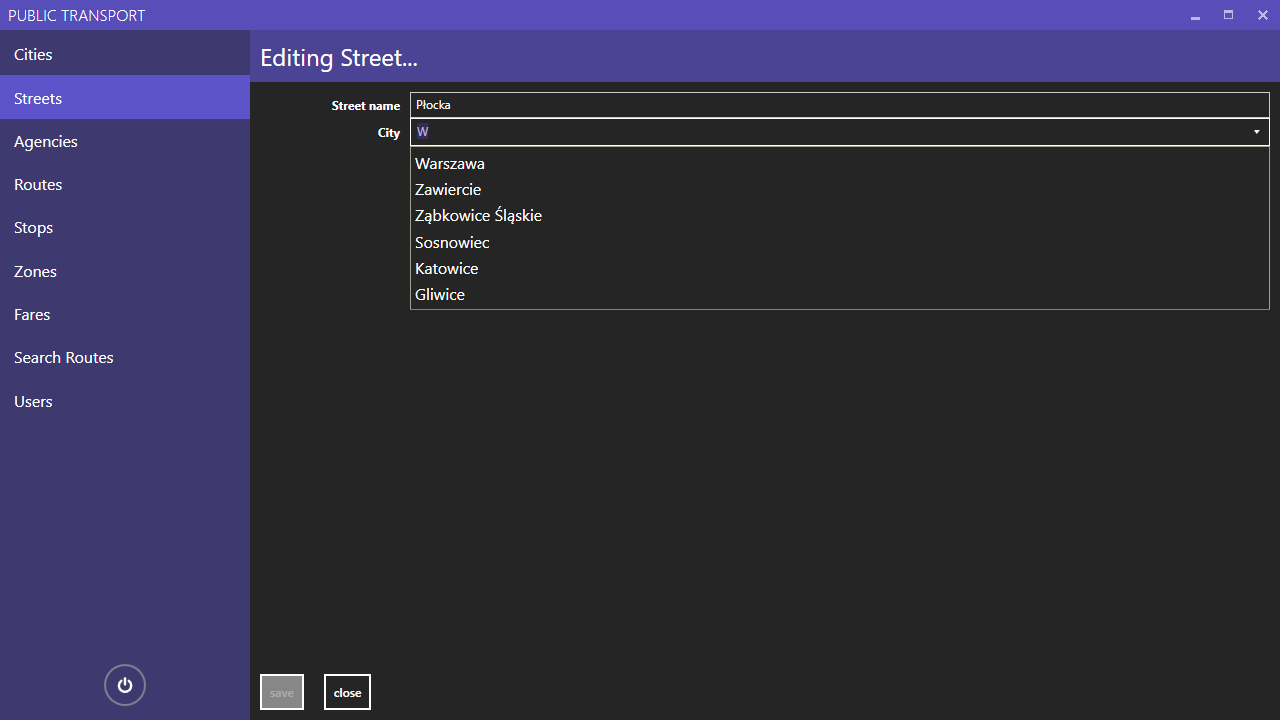
\includegraphics[width=15cm]{Resources/Images/06_edit_street.png}
	\caption{Przykład podpowiedzi}
\end{figure}
Na dole ekranu znajdują się przyciski zapisu (\textbf{Save}) umożliwiający zatwierdzenie zmian oraz zamknięcia (\textbf{Close}), który pozwala na cofnięcie się do widoku wyszukiwania i odrzucenie ostatnich zmian. W przypadku próby zapisu obiektu, który nie ma wypełnionych wszystkich pól, pojawia się poniżej przedstawiony pasek z wiadomością o błędzie:
\begin{figure}[H]
	\centering
	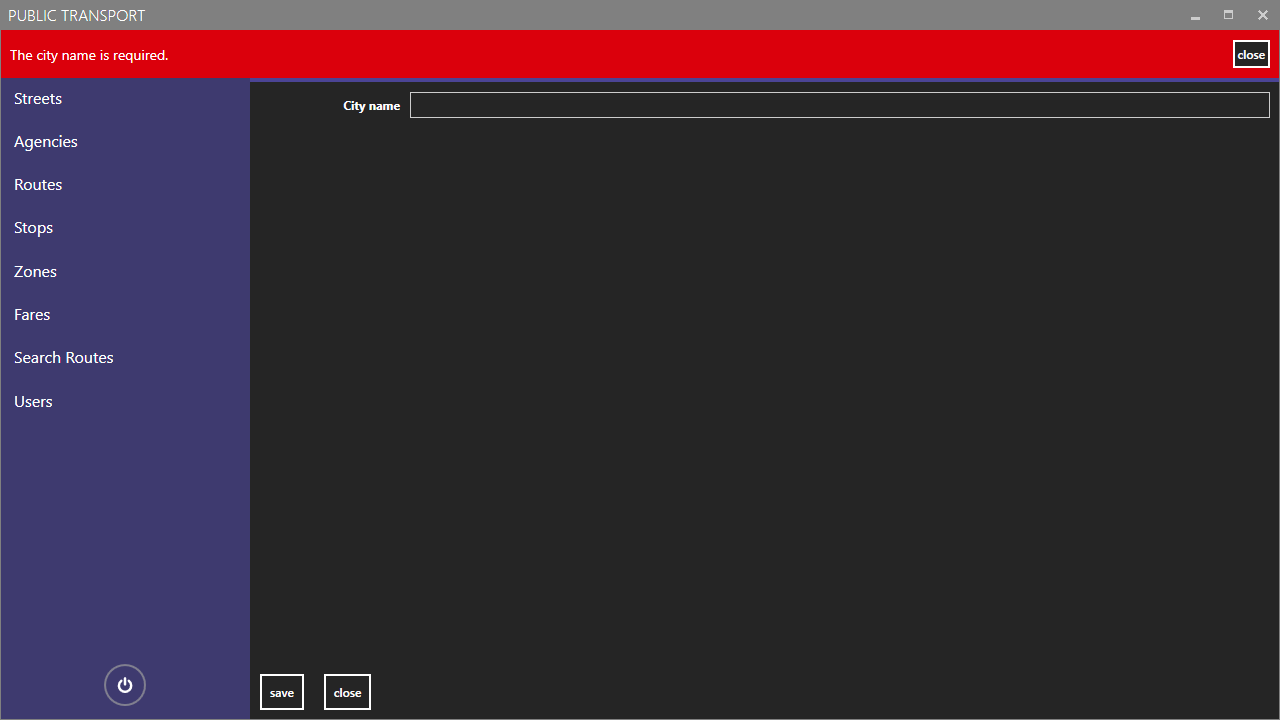
\includegraphics[width=15cm]{Resources/Images/21_not_all_fields.png}
	\caption{Błąd zapisu}
\end{figure}

\paragraph{Wyświetlanie rozkładu jazdy wybranej linii}
Szczególnym widokiem aplikacji jest widok rozkładu jazdy wybranej linii transportowej. Aby wyświetlić rozkład, należy przejść do zakładki \textbf{Routes}, wyszukać i wybrać jedną z tras, i wreszcie wybrać przycisk \textbf{View Timetable}.
\begin{figure}[H]
	\centering
	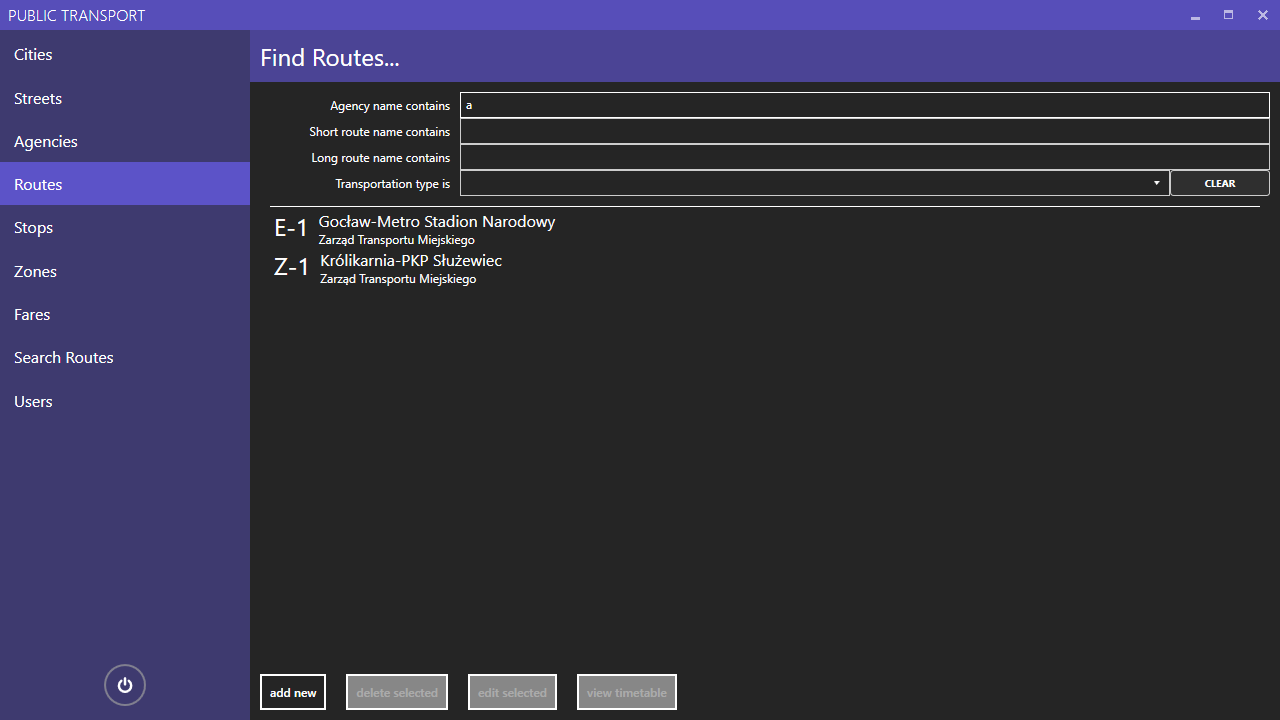
\includegraphics[width=15cm]{Resources/Images/09_filter_route.png}
	\caption{Widok tras z przyciskiem wyświetlania rozkładu}
\end{figure}
Widok rozkładu podzielony jest na dwie części. Po lewej stronie znajdują się poszczególne przystanki, między którymi kursuje wybrana trasa. Po wybraniu konkretnego przystanku, po prawej stronie pojawiają się czasy przyjazdu i odjazdu wszystkich kursów tej linii dotyczące wybranej opcji.
\begin{figure}[H]
	\centering
	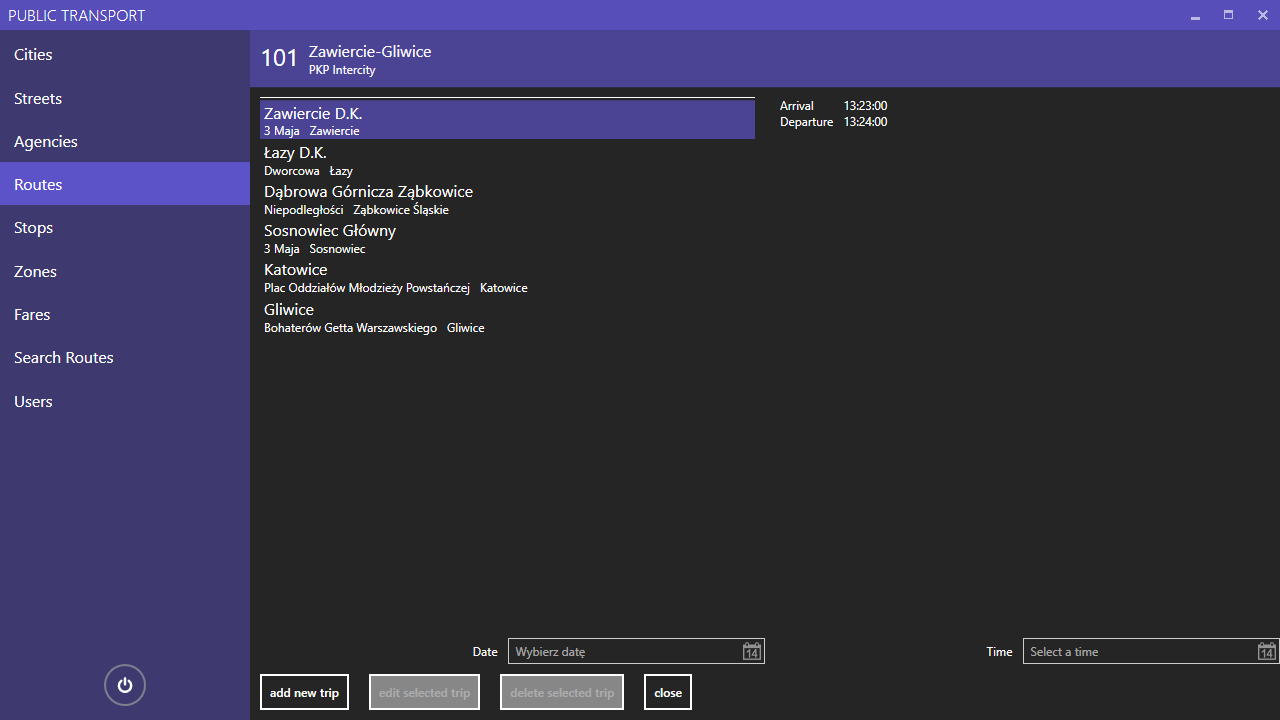
\includegraphics[width=15cm]{Resources/Images/10_timetable.png}
	\caption{Widok rozkładu jazdy}
\end{figure}
Pod listami przystanków i godzin widoczne są jeszcze dwa pola, które umożliwiają wyszukiwanie połączeń w konkretnych dniach oraz o godzinach późniejszych niż godzina wybrana w polu \textbf{Time}. Dodatkowo, dostępne są opcje dodawania (\textbf{Add Trip}), edycji (\textbf{Edit Trip}) oraz usuwania (\textbf{Delete Trip}) wybranego przejazdu.

\paragraph{Wyświetlanie rozkładu jazdy dla wybranego przystanku}
W podobny sposób można wyświetlić rozkład jazdy wszystkich linii dla jednego z przystanków, wybierając zakładkę \textbf{Stops}, wyszukując i wybierając jeden z przystanków, i wciskając przycisk \textbf{View Timetable}.
\begin{figure}[H]
	\centering
	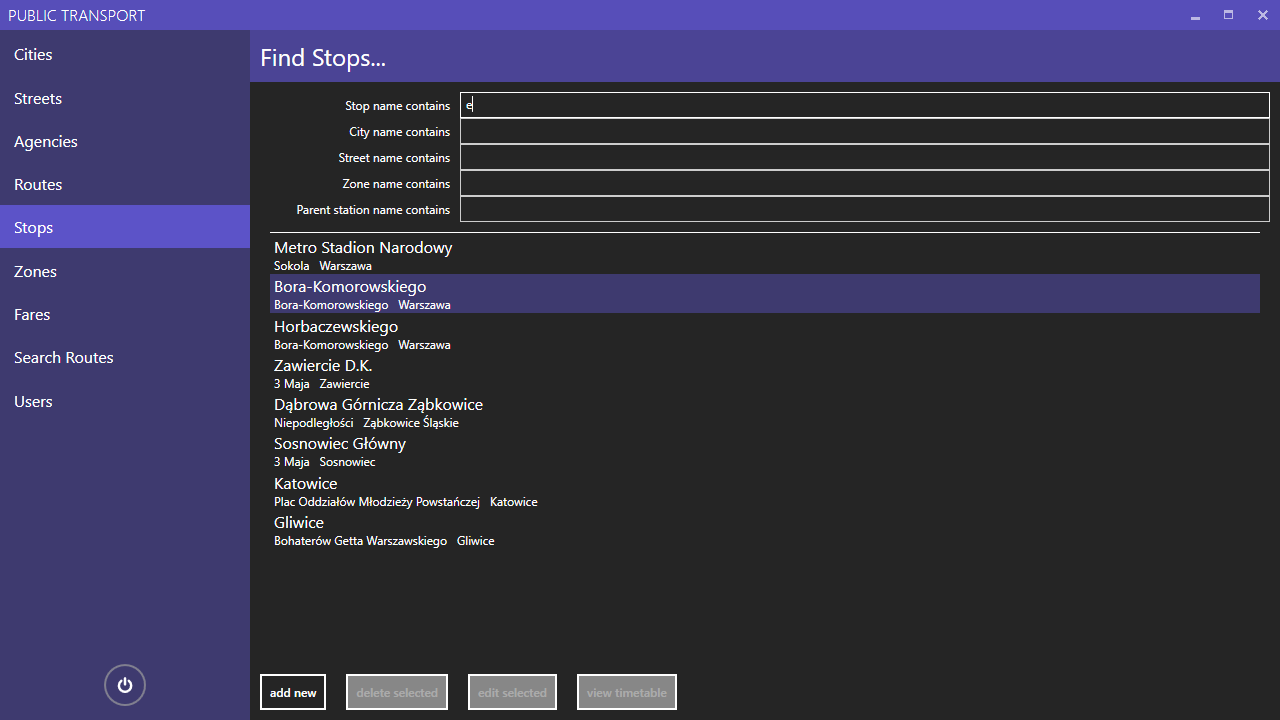
\includegraphics[width=15cm]{Resources/Images/13_filter_stops.png}
	\caption{Widok przystanków z przyciskiem wyświetlania rozkładu}
\end{figure}
\begin{figure}[H]
	\centering
	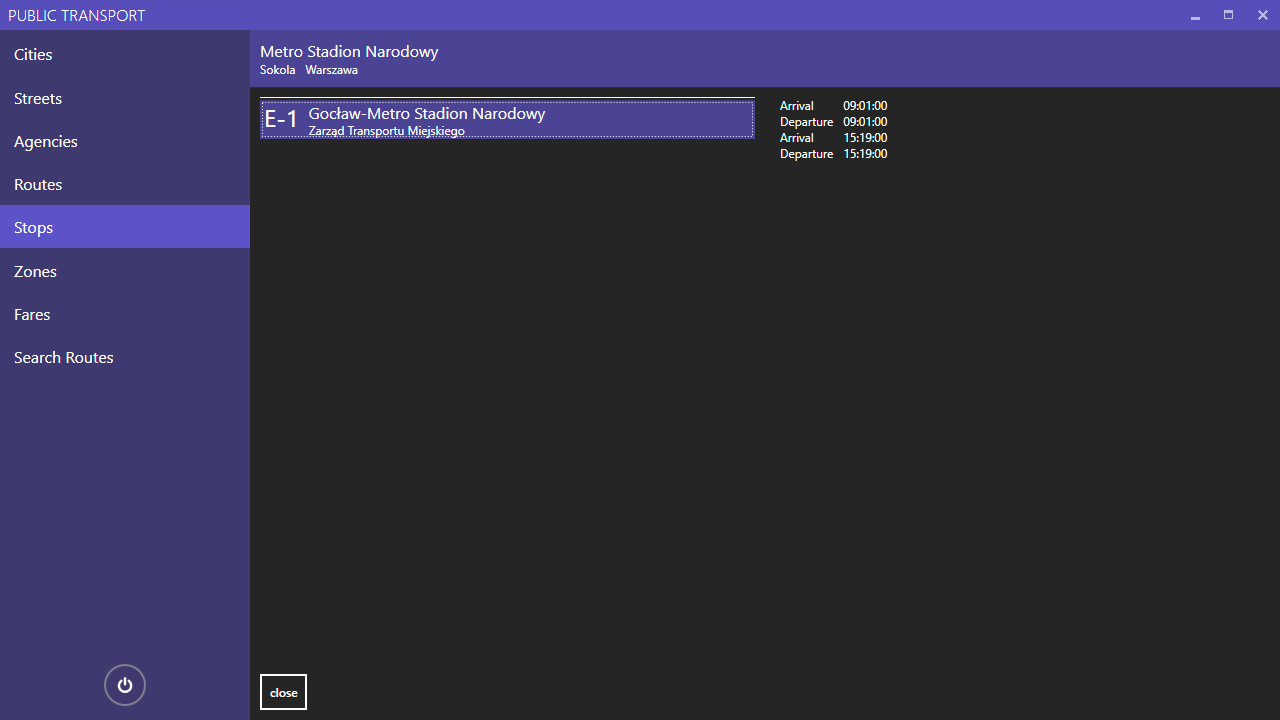
\includegraphics[width=15cm]{Resources/Images/22_stop_timetable.PNG}
	\caption{Rozkład jazdy dla wybranego przystanku}
\end{figure}

\paragraph{Edycja przejazdu}
Poniżej widoczny jest ekran edycji pojedynczego kursu.
\begin{figure}[H]
	\centering
	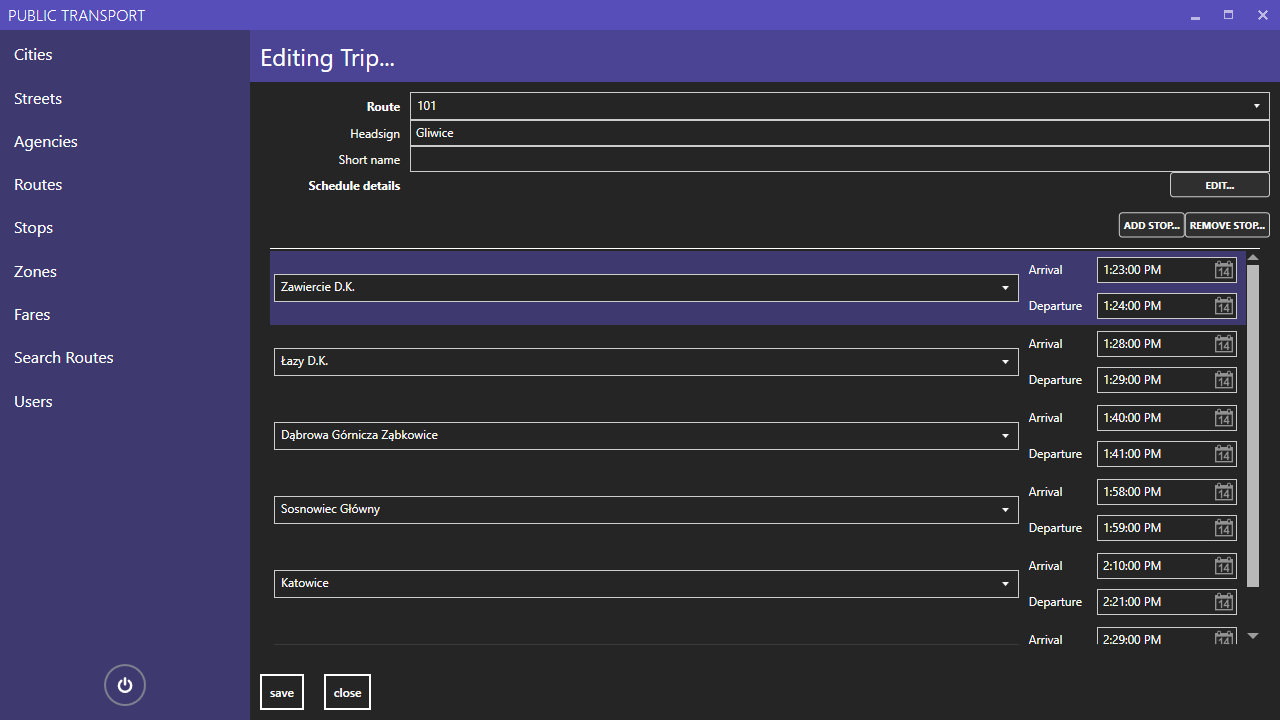
\includegraphics[width=15cm]{Resources/Images/11_edit_trip.png}
	\caption{Widok edycji przejazdu}
\end{figure}
Przewijana lista w dolnej części ekranu zawiera informacje o kolejnych przystankach edytowanego przejazdu oraz czasach przyjazdu i odjazdu. Można dodawać oraz usuwać przystanki za pomocą opcji \textbf{Add stop...} i \textbf{Remove stop...} 

Przycisk \textbf{Edit...} obok etykiety \textbf{Schedule details} pozwala na edycję informacji o harmonogramie danego kursu, takich, jak: pierwszy i ostatni dzień funkcjonowania kursu oraz dni tygodnia, w które odbywa się dany przejazd.
\begin{figure}[H]
	\centering
	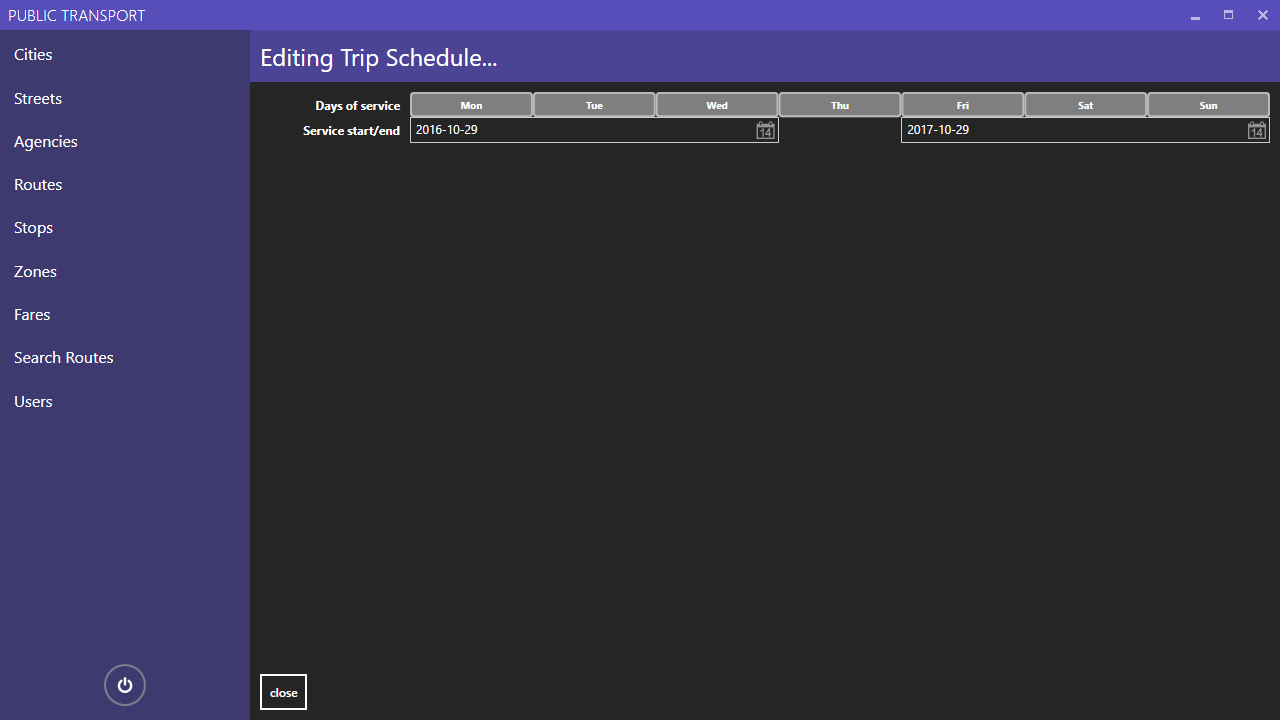
\includegraphics[width=15cm]{Resources/Images/12_edit_schedule.png}
	\caption{Widok edycji harmonogramu}
\end{figure}

\paragraph{Wyszukiwanie tras między wybranymi przystankami}
Aplikacja umożliwia wyszukiwanie tras przejeżdżających przez wybrane przystanki. Funkcjonalność ta dostępna jest z poziomu opcji \textbf{Search Routes} po lewej stronie okna.
\begin{figure}[H]
	\centering
	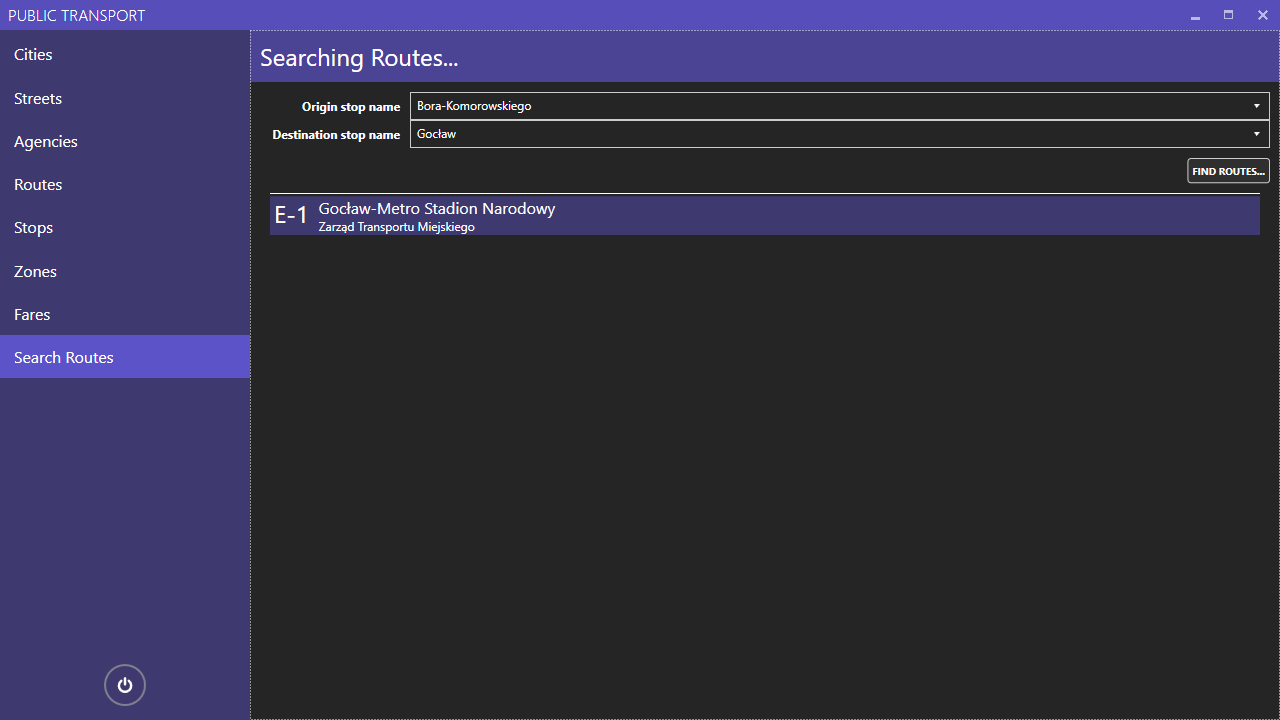
\includegraphics[width=15cm]{Resources/Images/23_search_routes.PNG}
	\caption{Widok wyszukiwania tras}
\end{figure}
Aby dokonać wyszukiwania, należy wpisać nazwy przystanków: startowego oraz docelowego w pola \textbf{Origin stop name} oraz \textbf{Destination stop name} odpowiednio, wybrać jeden z sugerowanych elementów, a następnie wcisnąć przycisk \textbf{Find Routes}.

\paragraph{Edycja użytkowników}
Konta administratorów mają dostęp również do widoku edycji użytkowników.
\begin{figure}[H]
	\centering
	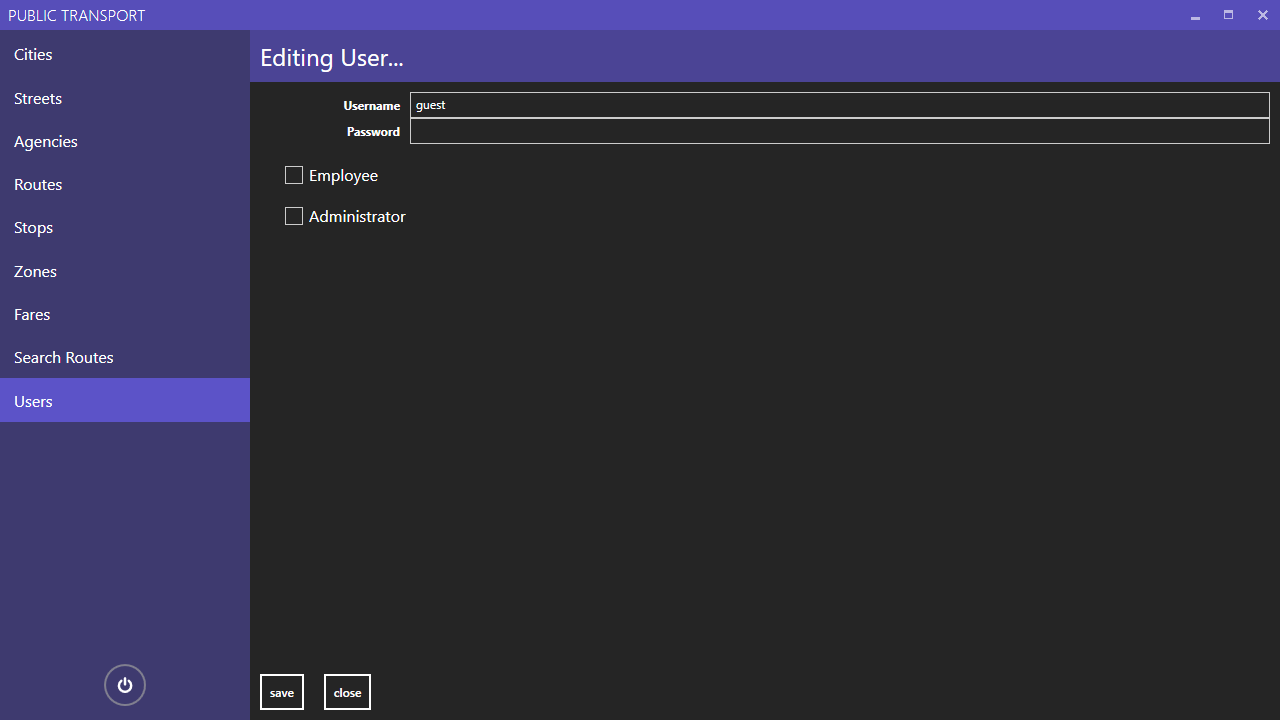
\includegraphics[width=15cm]{Resources/Images/19_edit_user.png}
	\caption{Widok edycji użytkowników}
\end{figure}
W widoku tym można przydzielać oraz odbierać danym użytkownikom role oraz resetować ich hasło, podając hasło tymczasowe (nie ma możliwości wyświetlenia hasła danego użytkownika). Aby zmiany zostały wprowadzone, dany użytkownik musi wylogować się z aplikacji i zalogować się ponownie.

\subsubsection{Aplikacja webowa}

\paragraph{Strona główna -- wyszukiwanie połączeń}
\begin{figure}[H]
	\centering
	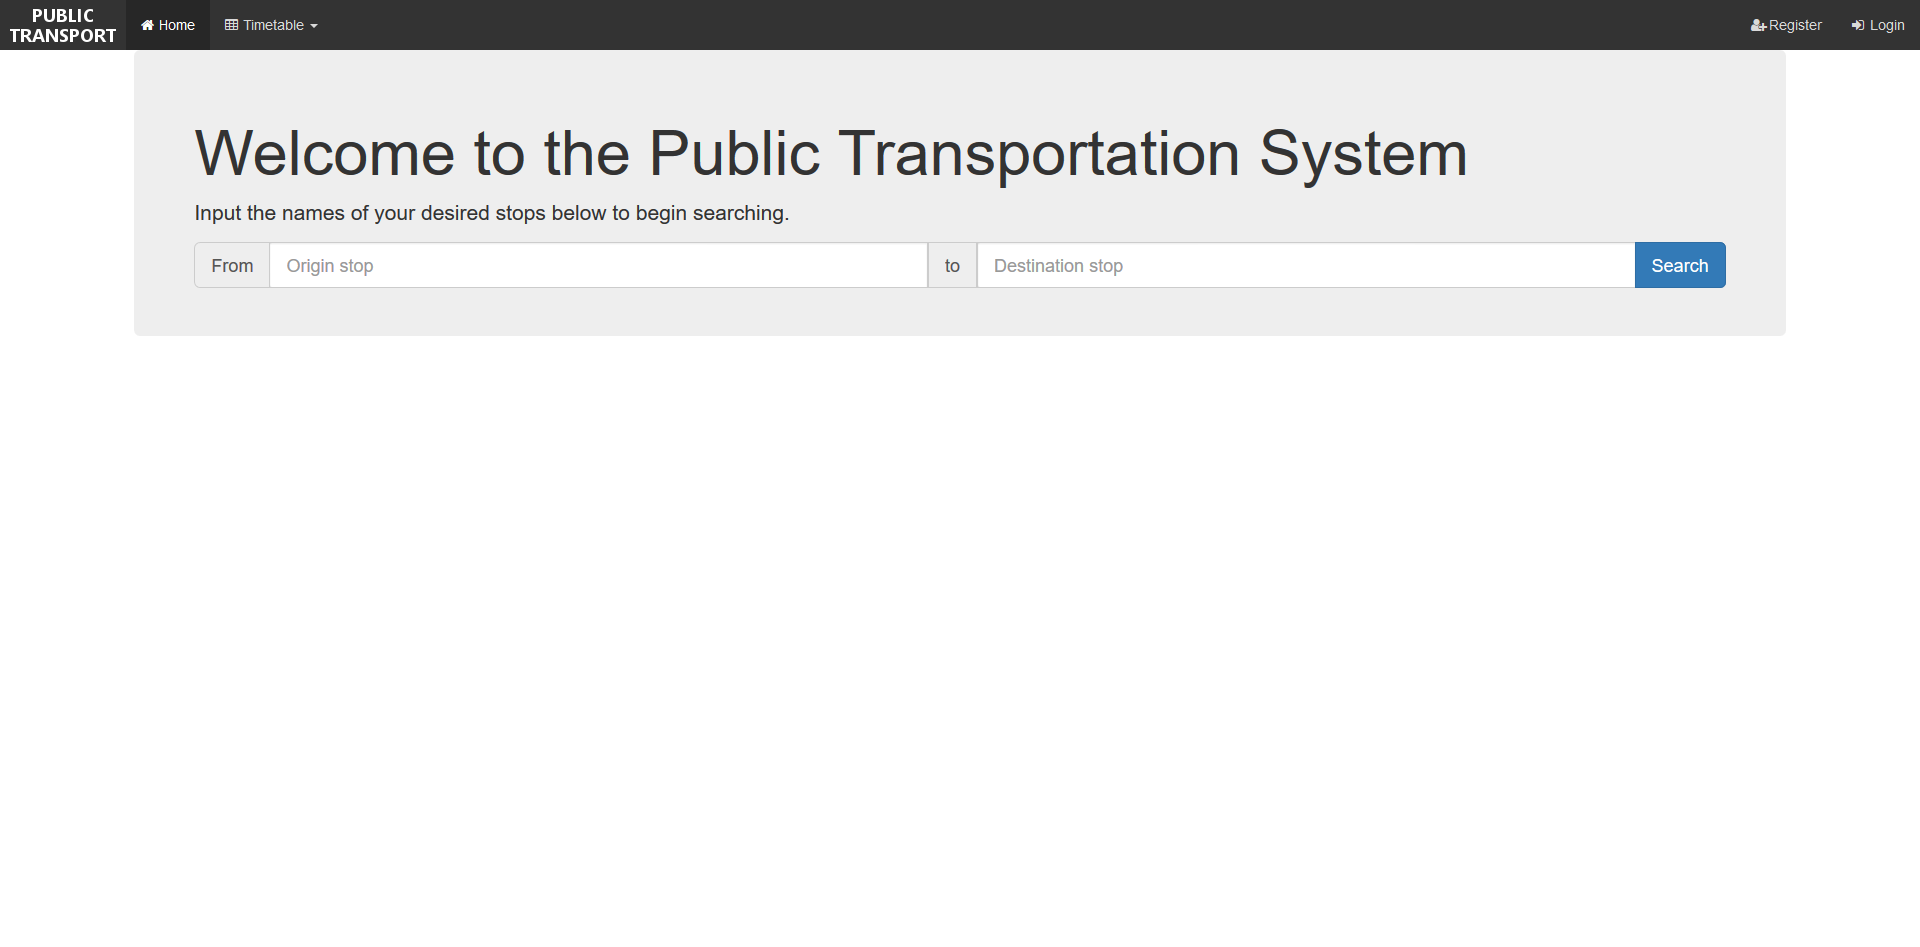
\includegraphics[width=15cm]{Resources/Images/24_main_page.png}
	\caption{Strona główna aplikacji}
\end{figure}
Strona główna aplikacji webowej składa się z paska nawigacyjnego, umożliwiającego przejście do pozostałych podstron witryny, oraz widoku głównego, odpowiedzialnego za wyszukiwanie połączeń. Aby wyszukać połączenie między wybranymi przystankami, należy rozpocząć wprowadzanie ich nazw do odpowiednich pól tekstowych \textbf{From} i \textbf{To}; po około pół sekundy w menu rozwijanym pojawią się sugestie dla użytkownika. Właściwe wyszukiwanie dokonywane jest po wciśnięciu przycisku \textbf{Search}.
\begin{figure}[H]
	\centering
	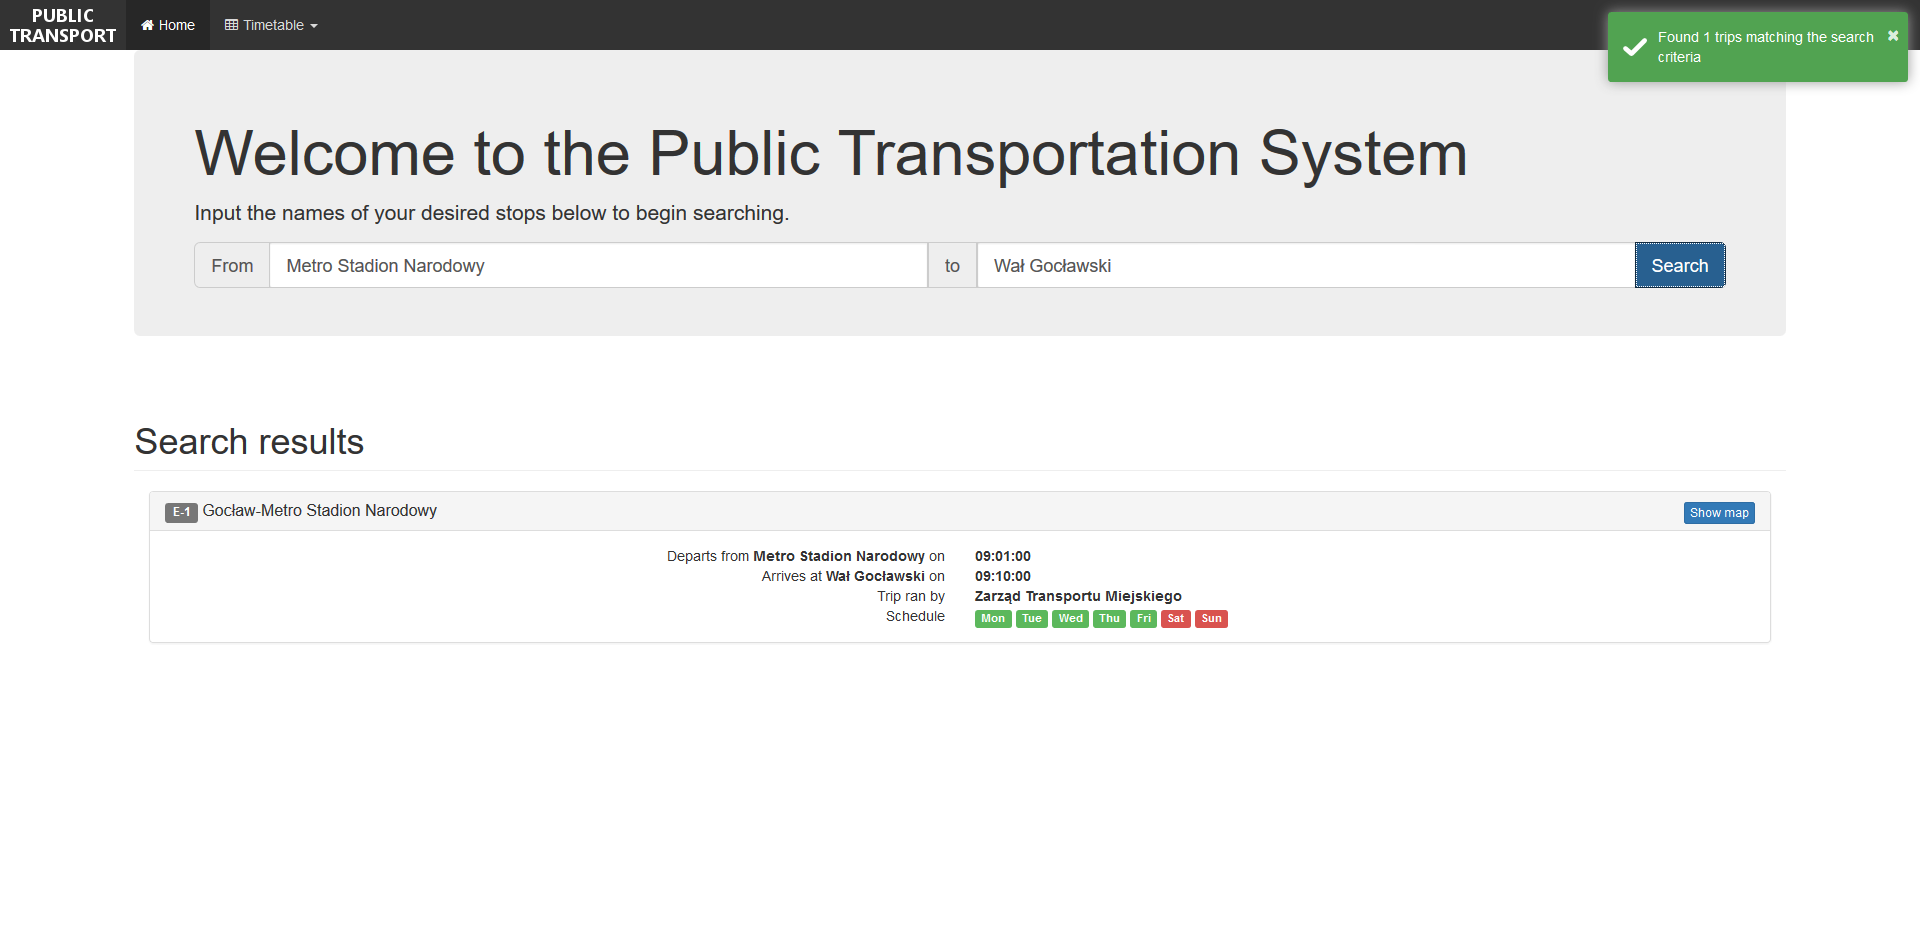
\includegraphics[width=15cm]{Resources/Images/26_main_search_results.png}
	\caption{Wyświetlone wyniki wyszukiwania}
\end{figure}
Po wciśnięciu przycisku \textbf{Search} ukaże się powiadomienie o sukcesie (lub braku połączeń spełniających podane kryteria) oraz wyniki wyszukiwania, zawierające informacje takie, jak: nazwa i identyfikator połączenia, godzina odjazdu z przystanku źródłowego, godzina przyjazdu na przystanek końcowy, nazwę agencji transportowej obsługującą połączenie oraz dni tygodnia, w które odbywa się kurs. Dodatkowo, po wciśnięciu przycisku \textbf{Show map} w prawym górnym rogu można wyświetlić w oknie modalnym trasę w postaci mapy.
\begin{figure}[H]
	\centering
	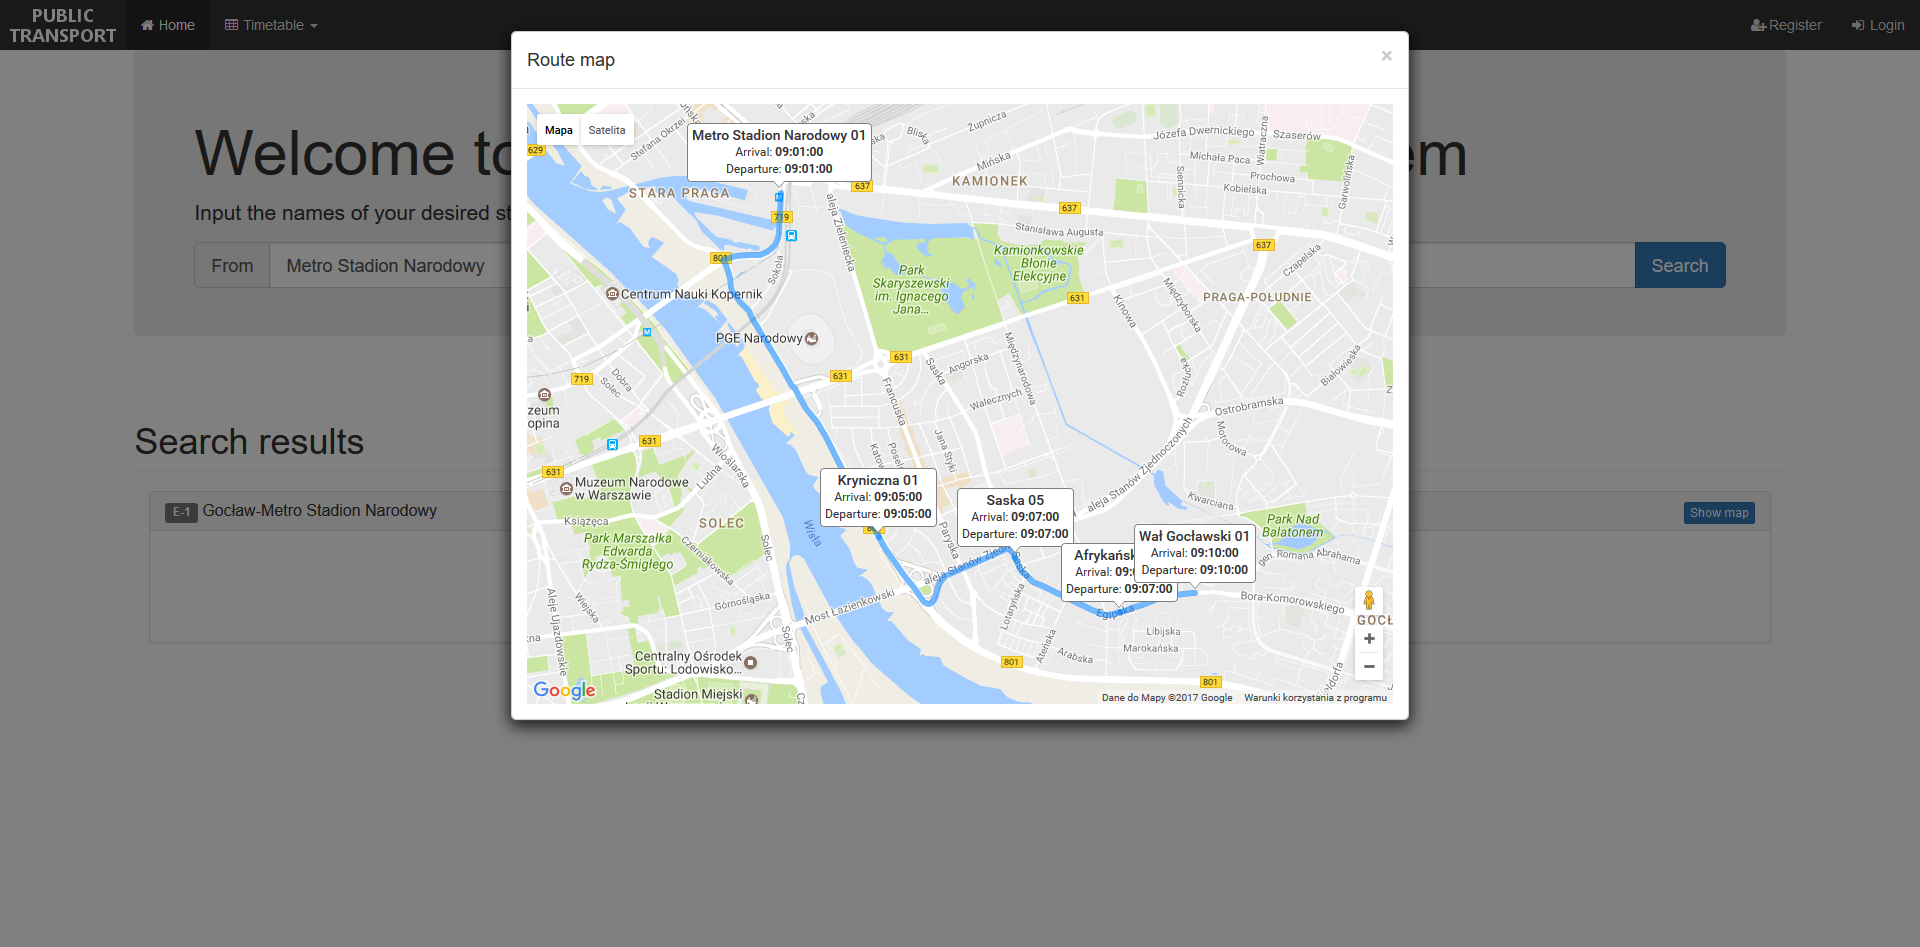
\includegraphics[width=15cm]{Resources/Images/27_map.png}
	\caption{Widok mapy}
\end{figure}

\paragraph{Rozkłady jazdy}
Wybierając w menu nawigacyjnym u góry opcję \textbf{Timetable}, otrzymujemy dostęp do menu rozwijanego umożliwiającego przejście do widoków odpowiedzialnych za wyświetlanie rozkładów jazdy dla poszczególnych przystanków (\textbf{Search by stop}) oraz tras (\textbf{Search by route}). Po wybraniu jednej z tych opcji nastąpi przejście do widoku składającego się z dwóch części. Po lewej znajduje się pole tekstowe, w które należy wpisać nazwę wyszukiwanej trasy; po kliknięciu przycisku \textbf{Filter} poniżej pola pojawi się lista tras, których nazwa zawiera wprowadzony ciąg znaków.
\begin{figure}[H]
	\centering
	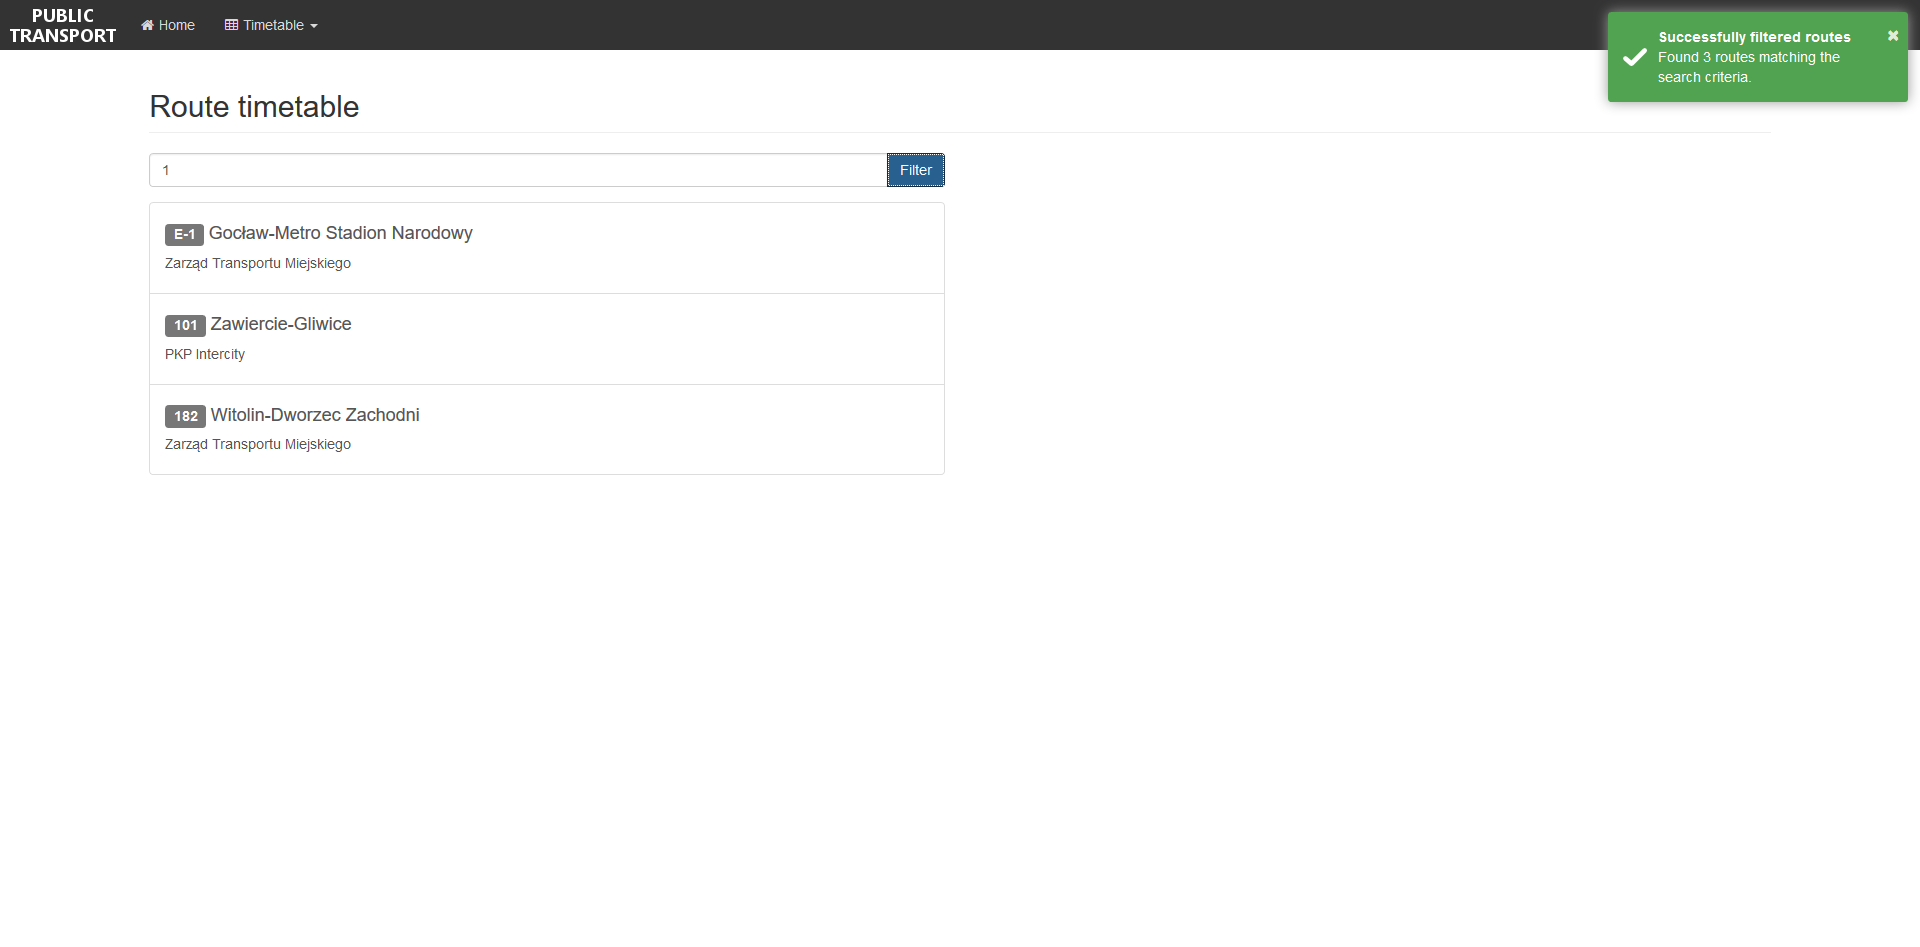
\includegraphics[width=15cm]{Resources/Images/28_stops_timetable.png}
	\caption{Wyszukiwanie rozkładów dla tras}
\end{figure}
Kliknięcie na dowolny z wyników wyszukiwania spowoduje pojawienie się po prawej stronie ekranu menu rozwijanego, z którego można wybrać przystanek trasy, dla którego chcemy sprawdzić rozkład jazdy. Po wybraniu jednej z opcji menu rozkład pojawi się poniżej w formie tabeli.
\begin{figure}[H]
	\centering
	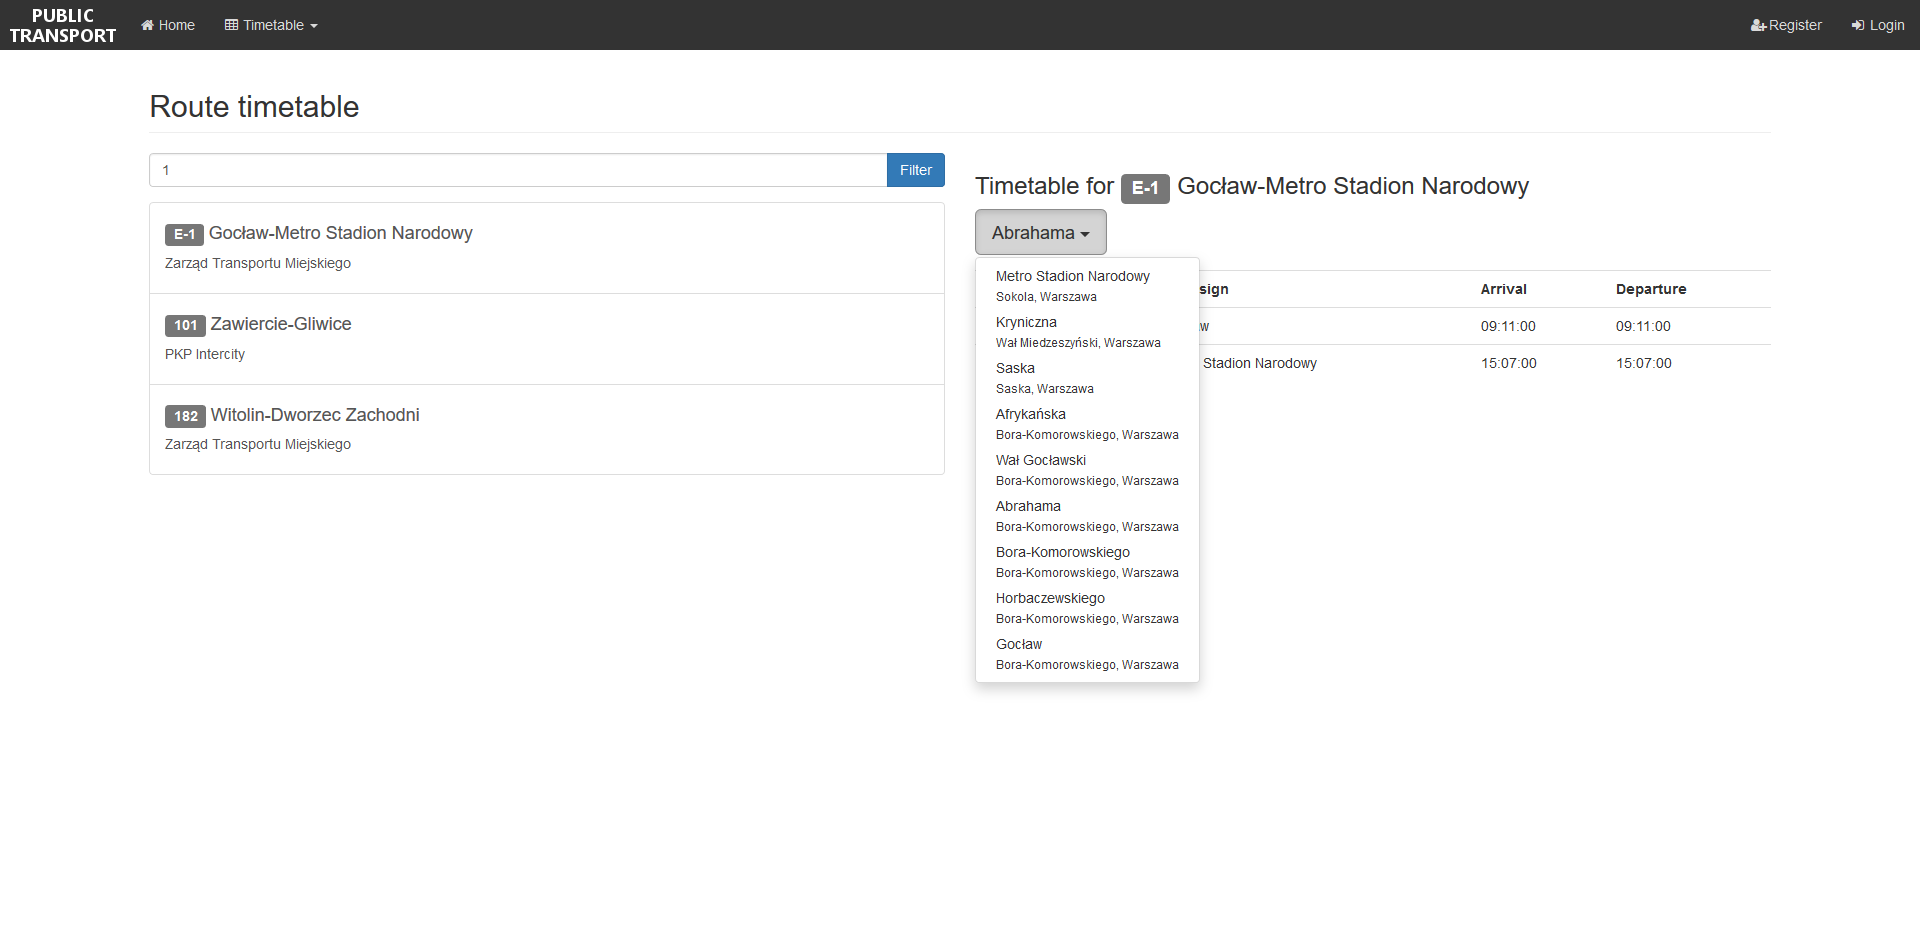
\includegraphics[width=15cm]{Resources/Images/29_select_stop.png}
	\caption{Menu rozwijane wyboru przystanku i widok rozkładu}
\end{figure}

\paragraph{Rejestracja}
Aby utworzyć konto w serwisie, należy wybrać opcję \textbf{Register} na pasku nawigacyjnym.
\begin{figure}[H]
	\centering
	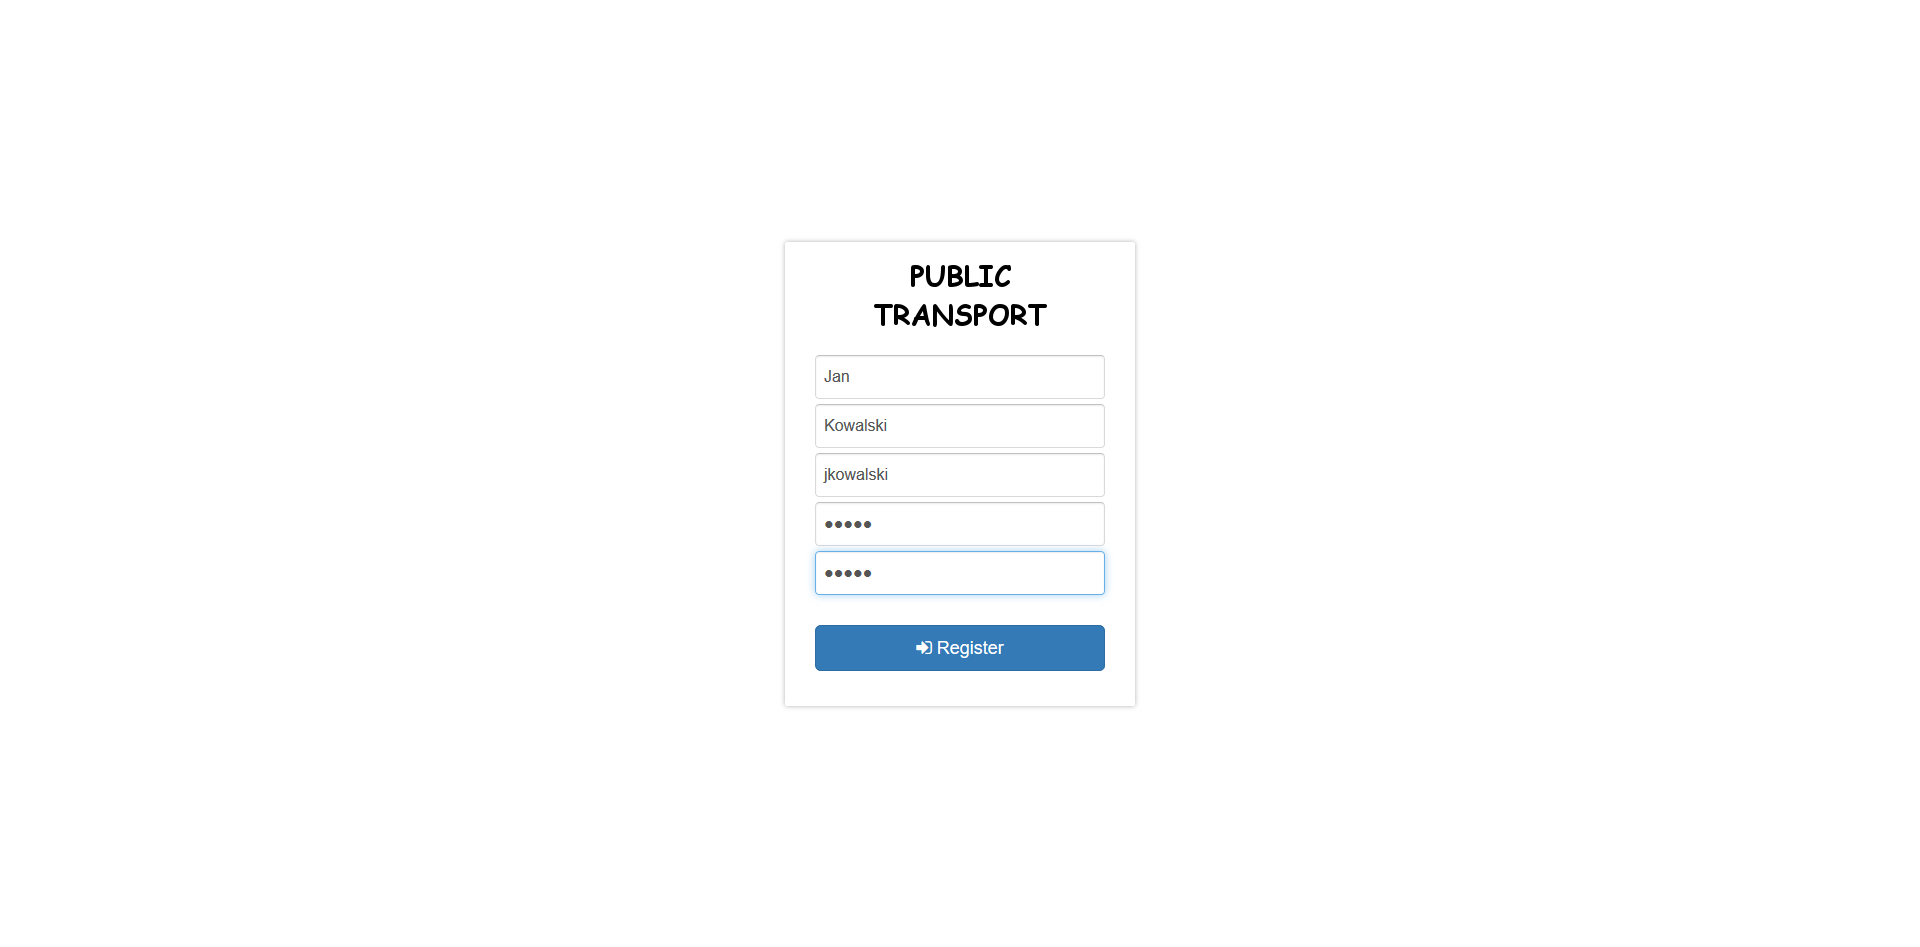
\includegraphics[width=15cm]{Resources/Images/30_registration.png}
	\caption{Okno rejestracji}
\end{figure}
Użytkownik zostanie poproszony o wprowadzenie swojego imienia, nazwiska, żądanej nazwy konta oraz wprowadzenie i potwierdzenie hasła do konta. Po pomyślnym wypełnieniu formularza i wciśnięciu przycisku \textbf{Register} użytkownik otrzyma powiadomienie, że może zalogować się już do swojego konta.

\paragraph{Logowanie}
Opcja zalogowania się do serwisu jest dostępna pod przyciskiem \textbf{Login} na pasku nawigacyjnym.
\begin{figure}[H]
	\centering
	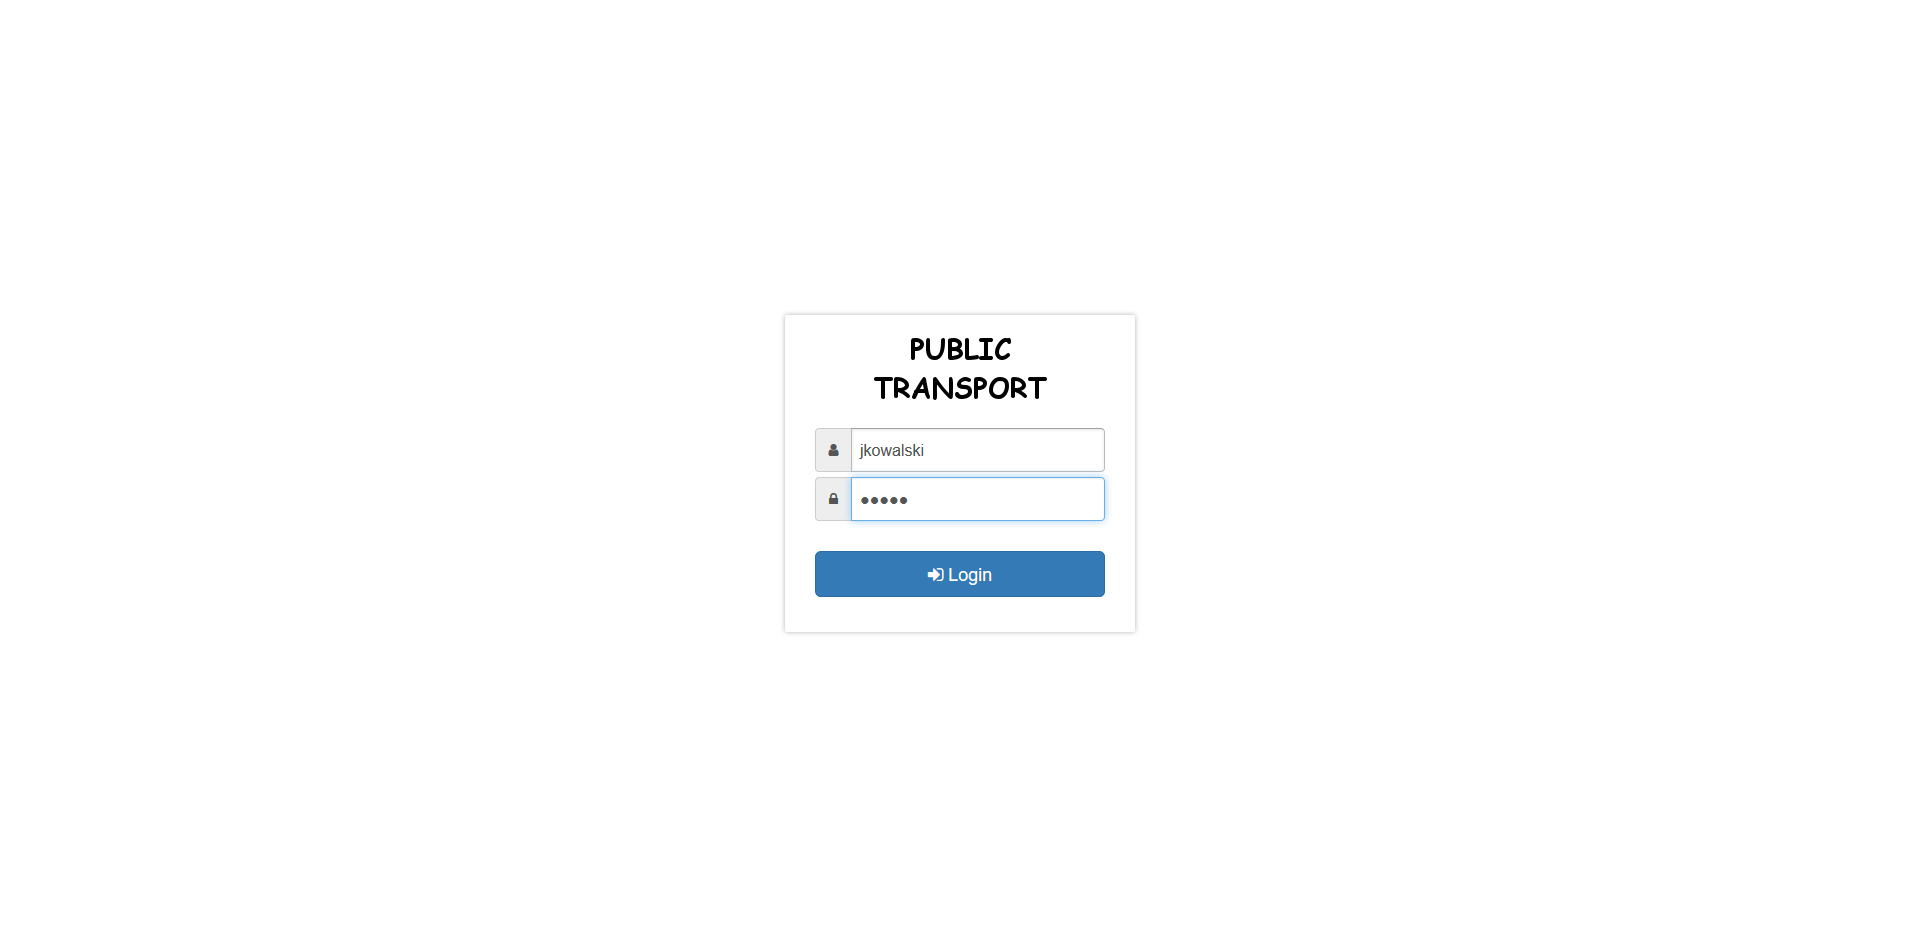
\includegraphics[width=15cm]{Resources/Images/31_login.png}
	\caption{Okno logowania}
\end{figure}
Po wprowadzeniu nazwy użytkownika oraz hasła użytkownik zostanie zalogowany do systemu.

Po zalogowaniu w prawym górnym rogu ekranu pojawi się menu rozwijane dla użytkownika, umożliwiające wylogowanie z systemu (\textbf{Logout}) oraz zmianę hasła za pomocą przycisku \textbf{Settings}.

\paragraph{Ulubione}
Zarejestrowani użytkownicy mają możliwość zapisywania wybranych tras oraz przystanków jako ulubione, aby uniknąć powtarzających się wyszukiwań. Aby zmodyfikować ulubione, po zalogowaniu się należy wybrać opcję \textbf{Favourites} na pasku nawigacyjnym.
\begin{figure}[H]
	\centering
	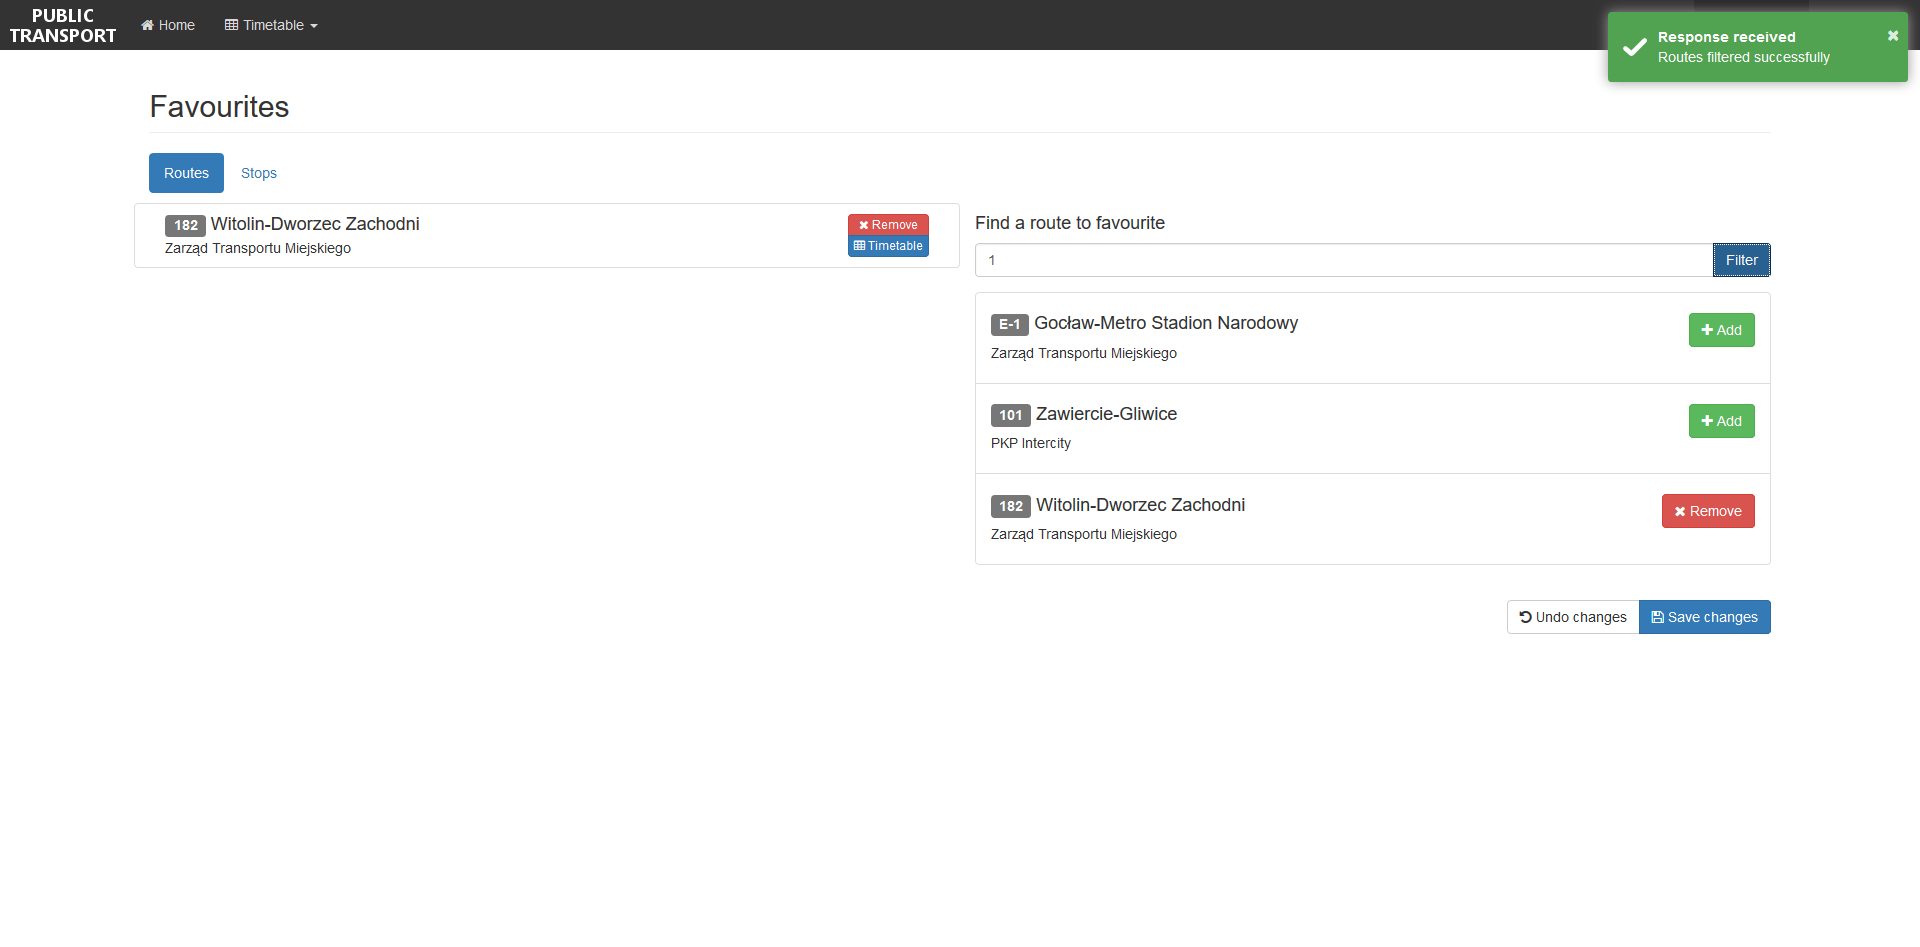
\includegraphics[width=15cm]{Resources/Images/32_favourites.png}
	\caption{Widok dodawania ulubionych}
\end{figure}
Pod nagłówkiem znajdują się dwa przyciski, które umożliwiają przełączanie się między zakładkami dla przystanków oraz tras. Po lewej stronie widoczne są obecne ulubione, zaś po prawej można wyszukać inne trasy i dodać (przycisk \textbf{Add}) lub usunąć (\textbf{Remove}) je z ulubionych. Aby zatwierdzić dokonane zmiany, należy wcisnąć przycisk \textbf{Save changes}; zmiany można też bezpiecznie cofnąć, klikając \textbf{Undo changes} lub opuszczając stronę bez kliknięcia przycisku \textbf{Save changes}.

Dodatkowo, dla tras lub przystanków wybranych jako ulubione, można bezpośrednio przejść do ich rozkładu jazdy, wybierając przycisk \textbf{Timetable}.

\subsection{Instrukcja utrzymania}
Uruchamianie, restartowanie lub zatrzymywanie serwera aplikacyjnego.
\begin{enumerate}
	\item Otwórz konsolę \textbf{IIS}.
	\item Wybierz swoją stronę (\textbf{Web Site}) po lewej stronie okna.
	\item Po prawej stronie okna wybierz jedną z opcji \textbf{Start, Stop} lub \textbf{Restart}.
\end{enumerate}
Uruchamianie, restartowanie lub zatrzymywanie serwera bazodanowego.
\begin{enumerate}
	\item Uruchom \textbf{SQL Server Configuration Manager}.
	\item Jeśli pojawi się okno dialogowe \textbf{Kontrola konta użytkownika}, kliknij przycisk \textbf{Tak}.
	\item Wybierz instancję serwera SQL (MSSQLSERVER), kliknij prawym przyciskiem myszy, a następnie wybierz jedną z opcji \textbf{Start, Stop, Pause, Resume} lub \textbf{Restart}.
\end{enumerate}
Tworzenie kopii zapasowej bazy danych.
\begin{enumerate}
	\item Połącz się z instancją serwera bazodanowego i w \textbf{Eksploratorze obiektów} przejdź do węzła \textbf{Databases}.
	\item Kliknij prawym przyciskiem bazę danych \textbf{PublicTransport}, przejdź do zakładki \textbf{Tasks}, a następnie \textbf{BackUp}.
	\item Zostanie wyświetlone okno dialogowe \textbf{Back Up Database}. W polu listy \textbf{Database} zweryfikuj nazwę bazy danych.
	\item W polu listy \textbf{Backup type} wybierz opcję \textbf{Full}.
	\item W obszarze \textbf{Backup component} kliknij opcję \textbf{Database}.
	\item Wybierz lokalizację docelową kopii zapasowej i wciśnij przycisk \textbf{OK}.
\end{enumerate}

\subsection{Raport odstępstw od specyfikacji wymagań}
Brak.

\subsection{Dokumentacja usług Web Services}
\begin{verbatim}
swagger: "2.0"
info:
  title: Public Transport
  version: 3.0.0
  contact:
    name: Bartłomiej Dach, Tymon Felski
    url: http://github.com/bdach/public-transport/
    email: dachb@student.mini.pw.edu.pl, felskit@student.mini.pw.edu.pl
host: localhost:49878
basePath: /api
definitions:
  Agency:
    type: object
    properties:
      Name:
        type: string
        description: The full name of the transit agency.
      Phone:
        type: string
        description: Contains a single voice telephone number for the specified agency.
        pattern: "[0-9+#]+"
      Url:
        type: string
        description: Contains the URL of the transit agency. The value must be a fully
                     qualified URL that includes `http://` or `https://` and any special
                     characters in the URL must be correctly escaped.
      Regon:
        type: string
        description: Contains the REGON number of the transit agency.
      StreetName:
        type: string
        description: Contains the name of the street the agency is located on.
      StreetNumber:
        type: string
        description: Contains the street number of the agency.
      CityName:
        type: string
        description: Contains the name of the city the agency is located in.
  ErrorMessage:
    type: object
    properties:
      Message:
        type: string
        description: Message detailing the error cause.
  FavouriteInfo:
    type: object
    properties:
      UserName:
        type: string
        required: true
        description: The username of the user sending the request to save changes to
                     the favourites.
      Changes:
        type: object
        request: true
        description: This is a key-value pair. The key is an integer indicating the ID
                     of a stop or route, and the value indicates whether the stop/route
                     should be added to the favourite list (true) or removed from
                     the list (false). This object can have multiple pairs.
  LoginData:
    type: object
    properties:
      UserName:
        type: string
        required: true
        description: The username of the user logging in.
      Password:
        type: string
        required: true
        description: The password of the user logging in.        
  MapMarker:
    type: object
    properties:
      Latitude:
        type: number
        minimum: 0
        maximum: 90
        exclusiveMaximum: false
        description: The latitude of the point represented by the marker.
      Longtitude:
        type: number
        minimum: -180
        maximum: 180
        exclusiveMaximum: false
        description: The longtitude of the point represented by the marker.
      DescriptionText:
        type: string
        description: String to be used as a description for the marker.
      ArrivalTime:
        type: string
        description: The time of arrival at the marker's location.
      DepartureTime:
        type: string
        description: The time of departure at the marker's location.
  PasswordChangeRequest:
    type: object
    properties:
      UserName:
        type: string
        description: The username of the user requesting a password change.
        required: true
      OldPassword:
        type: string
        description: The user's old password.
        required: true
      NewPassword:
        type: string
        description: The user's new password
        required: true
  RegistrationInfo:
    type: object
    properties:
      FullName:
        type: string
        description: The user's full name to be stored by the app.
        required: true
      UserName:
        type: string
        description: Username to be used by the user to log in to the app.
        required: true
      Password:
        type: string
        description: The user's desired password, to be used when logging in.
        required: true
  Route:
    type: object
    properties:
      Id:
        type: integer
        format: int64
        description: The ID number of the route.
      ShortName:
        type: string
        description: Contains the short name of a route. This often will be a short,
                     abstract identifier like "32", "100X" or "Green" that riders
                     use to identify a route, but which doesn't give any indication
                     of what places the route serves.
      LongName:
        type: string
        description: Contains the full name of a route. This name is generally more
                     descriptive than the short name and will often include
                     the route's destination or stop.
      RouteType:
        type: integer
        description: Describes the type of transportation used on a route.
        enum:
          - Tram
          - Subway
          - Rail
          - Bus
          - Ferry
      Agency:
        $ref: '#/definitions/Agency'
        description: Contains information about the agency operating the particular route.
  RouteFilter:
    type: object
    properties:
      AgencyNameFilter:
        type: string
        description: Agency name filter.
      LongNameFilter:
        type: string
        description: Route long name filter.
      ShortNameFilter:
        type: string
        description: Route short name filter.
      RouteTypeFilter:
        type: integer # these enums are borked rn - getting serialized into numbers
        	  and not strings
        enum:
          - Tram
          - Subway
          - Rail
          - Bus
          - Ferry
        description: Route type filter.
  RouteTimetableEntry:
    type: object
    properties:
      Key:
        $ref: '#/definitions/Route'
      Value:
        type: array
        items:
          $ref: '#/definitions/TimetableEntry'
  ServiceDetails:
    type: object
    properties:
      Monday:
        type: boolean
        description: Contains a binary value that indicates whether the service is valid
                     for all Mondays in the date range.
      Tuesday:
        type: boolean
        description: Contains a binary value that indicates whether the service is valid
                     for all Tuesdays in the date range.
      Wednesday:
        type: boolean
        description: Contains a binary value that indicates whether the service is valid
                     for all Wednesdays in the date range.
      Thursday:
        type: boolean
        description: Contains a binary value that indicates whether the service is valid
                     for all Thursdays in the date range.
      Friday:
        type: boolean
        description: Contains a binary value that indicates whether the service is valid
                     for all Fridays in the date range.
      Saturday:
        type: boolean
        description: Contains a binary value that indicates whether the service is valid
                     for all Saturdays in the date range.
      Sunday:
        type: boolean
        description: Contains a binary value that indicates whether the service is valid
                     for all Sundays in the date range.
      StartDate:
        type: string
        format: date-time
        description: Contains the start date for the service.
      EndDate:
        type: string
        format: date-time
        description: Contains the end date for the service.
  Stop:
    type: object
    properties:
      Id:
        type: integer
        format: int64
        description: Contains the ID of the stop.
      Name:
        type: string
        description: Contains the name of a stop or station.
      StreetName:
        type: string
        description: Contains the name of the street the stop is located on.
      CityName:
        type: string
        description: Contains the name of the city the stop is located in.
      ParentStation:
        $ref: '#/definitions/Stop'
        description: For stops that are physically located inside stations, this field
                     identifies the station associated with the stop. Used only if
                     the value of `IsStation` is false.
      IsStation:
        type: boolean
        description: Identifies whether this stop object represents a stop or station.
  StopFilter:
    type: object
    properties:
      StopNameFilter:
        type: string
        description: Contains the stop name string filter parameter.
      StreetNameFilter:
        type: string
        description: Contains the street name string filter parameter.
      CityNameFilter:
        type: string
        description: Contains the city name string filter parameter.
      ZoneNameFilter:
        type: string
        description: Contains the zone name string filter parameter.
      ParentStationNameFilter:
        type: string
        description: Contains the parent station name string filter parameter.
      OnlyStations:
        type: boolean
        description: Limits the search query only to stops which are stations.
  StopTimetableEntry:
    type: object
    properties:
      Key:
        $ref: '#/definitions/Route'
      Value:
        type: array
        items:
          $ref: '#/definitions/TimetableEntry'
  TimetableEntry:
    type: object
    properties:
      ArrivalTime:
        type: string
        format: date-time
        description: Specifies the arrival time at a specific stop for a specific
                     trip on a route.
      DepartureTime:
        type: string
        format: date-time
        description: Specifies the departure time at a specific stop for a specific
                     trip on a route.
      ShortName:
        type: string
        description: Contains the text that appears in   schedules and sign boards
                     to identify the trip to passengers, for example, to identify
                     train numbers for commuter rail trips. If riders do not commonly
                     rely on trip names, this field will be left blank.
      Headsign:
        type: string
        description: Contains the text that appears on a sign that identifies
                     the trip's destination to passengers. This field is used to
                     distinguish between different patterns of service in
                     the same route.
      Direction:
        type: boolean
        description: Contains a binary value that indicates the direction of travel
                     for a trip. Use this field to distinguish between bi-directional
                     trips on the same route. This field is not used for routing;
                     it provides a way to separate trips by direction when publishing
                     time tables.
  TripInfo:
    type: object
    properties:
      Id:
        type: integer
        format: int64
        description: The ID of the trip.
      OriginStop:
        $ref: '#/definitions/TripStop'
      DestinationStop:
        $ref: '#/definitions/TripStop'
      Route:
        $ref: '#/definitions/Route'
      ServiceDetails:
        $ref: '#/definitions/ServiceDetails'
  TripSearchFilter:
    type: object
    properties:
      OriginStopIdFilter:
        type: integer
        format: int64
        required: true
        description: The ID of the origin stop.
      DestinationStopIdFilter:
        type: integer
        format: int64
        required: true
        description: The ID of the destination stop.
  TripSegmentFilter:
    type: object
    properties:
      TripId:
        type: integer
        format: int64
        required: true
        min: 1
        description: The ID of the trip for which to display the segment.
      OriginSequenceNumber:
        type: integer
        format: int64
        required: true
        description: The lower bound of the sequence numbers in the trip.
      DestinationSequenceNumber:
        type: integer
        format: int64
        required: true
        description: The upper bound of the sequence numbers in the trip.
  TripStop:
    type: object
    properties:
      Stop:
        $ref: '#/definitions/Stop'
      ArrivalTime:
        type: string
        format: date-time
        description: Specifies the arrival time at a specific stop for a specific trip
                     on a route.
      DepartureTime:
        type: string
        format: date-time
        description: Specifies the departure time at a specific stop for a specific trip
                     on a route.
      SequenceNumber:
        type: integer
        format: int64
        description: Identifies the order of the stops for a particular trip. The values
                     must be non-negative integers, and they must increase along the trip.
  UserInfo:
    type: object
    properties:
      FullName:
        type: string
        required: true
        description: The full name of the user.
      UserName:
        type: string
        required: true
        description: The username of the user.
      Token:
        type: string
        required: true
        description: Assigned OAuth token used for request authentication.
      Roles:
        type: array
        required: true
        items:
          type: integer
          enum:
            - Employee
            - Administrator
          description: Contains the roles of the user.
paths:
  # leaving login for now
  /route/filter:
    post:
      description: Searches for routes in the database, using the supplied filtering
                   criteria; at least one of the fields must be non-empty
      consumes:
        - application/json
      produces:
        - application/json
      parameters:
        - name: routeFilter
          in: body
          required: true
          description: Object containing the desired filtering criteria.
          schema:
            $ref: '#/definitions/RouteFilter'
      responses:
        '200':
          description: Array containing routes which meet the supplied criteria.
          schema:
            type: array
            items:
              $ref: "#/definitions/Route"
        '400':
          description: The supplied filter is invalid.
          schema:
            $ref: "#/definitions/ErrorMessage"
  /session:
    get:
      description: Retrieves the user's previous session if it hasn't expired.
      produces:
        - application/json
      parameters:
        - name: Authorization
          in: header
          required: true
          description: OAuth token.
          type: string
      responses:
        '200':
          description: The user's previous session data.
          schema:
            $ref: '#/definitions/UserInfo'
        '401':
          description: The supplied authentication token has expired.
          schema:
            $ref: '#/definitions/ErrorMessage'
  /stop/filter:
    post:
      description: Searches for stops in the database, using the supplied filtering
                   criteria; at least one of the fields must be non-empty
      consumes:
        - application/json
      produces:
        - application/json
      parameters:
        - name: stopFilter
          in: body
          required: true
          description: Object containing the desired filtering criteria.
          schema:
            $ref: '#/definitions/StopFilter'
      responses:
        '200':
          description: Array containing stops which meet the supplied criteria.
          schema:
            type: array
            items:
              $ref: '#/definitions/Stop'
  /timetable/stop/{stopId}:
    get:
      description: Fetches a timetable for the stop with the supplied ID number
      produces:
        - application/json
      parameters:
        - name: stopId
          in: path
          required: true
          description: The ID of the stop for which to fetch the timetable.
          type: integer
      responses:
        '200':
          description: Array containing the timetable data.
          schema:
            type: array
            items:
              $ref: '#/definitions/StopTimetableEntry'
  /timetable/route/{routeId}:
    get:
      description: Fetches a timetable for the route with the supplied ID number
      produces:
        - application/json
      parameters:
        - name: routeId
          in: path
          required: true
          description: The ID of the route for which to fetch the timetable.
          type: integer
      responses:
        '200':
          description: Array containing the timetable data.
          schema:
            type: array
            items:
              $ref: '#/definitions/RouteTimetableEntry'
  /token:
    post:
      description: Fetches user information along with an authentication token
                   for the desired user.
      consumes:
        - application/json
      produces:
        - application/json
      parameters:
        - name: loginData
          in: body
          required: true
          description: The object containing the login information.
          schema:
            $ref: '#/definitions/LoginData'
      responses:
        '200':
          description: Returns the user information for the desired user.
          schema:
            $ref: '#/definitions/UserInfo'
        '401':
          description: The supplied credentials were invalid.
          schema:
            $ref: '#/definitions/ErrorMessage'
  /trip/mapData:
    post:
      description: Returns a list of map markers representing a part of the desired trip
      consumes:
        - application/json
      produces:
        - application/json
      parameters:
        - name: tripSegmentFilter
          in: body
          required: true
          description: The object containing the query parameters.
          schema:
            $ref: '#/definitions/TripSegmentFilter'
      responses:
        '200':
          description: A list of map markers representing the requested part of the trip.
          schema:
            type: array
            items:
              $ref: '#/definitions/MapMarker'
        '400':
          description: The request sent by the user was invalid.
          schema:
            $ref: '#/definitions/ErrorMessage'
  /trip/search:
    post:
      description: Returns a list of trips that run between the two specified stops,
                   along with their arrival/destination times and service
                   availability information
      consumes:
        - application/json
      produces:
        - application/json
      parameters:
        - name: tripSearchFilter
          in: body
          required: true
          description: The object containing the query parameters.
          schema:
            $ref: '#/definitions/TripSearchFilter'
      responses:
        '200':
          description: A list of trips running through the desired stops.
          schema:
            type: array
            items:
              $ref: '#/definitions/TripInfo'
        '400':
          description: The request sent by the user was invalid.
          schema:
            $ref: "#/definitions/ErrorMessage"
  /user/changepassword:
    post:
      description: Allows a user to change their account password
      consumes:
        - application/json
      produces:
        - application/json
      parameters:
        - name: passwordChangeRequest
          in: body
          required: true
          description: Object containing request data.
          schema:
            $ref: '#/definitions/PasswordChangeRequest'
      responses:
        '200':
          description: The user's password was successfully changed.
        '400':
          description: The request sent by the user was invalid.
          schema:
            $ref: "#/definitions/ErrorMessage"
  /user/register:
    post:
      description: Registers a user for the application
      consumes:
        - application/json
      produces:
        - application/json
      parameters:
        - name: registrationInfo
          in: body
          required: true
          description: Object storing the registration request data
          schema:
            $ref: '#/definitions/RegistrationInfo'
      responses:
        '200':
          description: The user was registered successfully.
        '400':
          description: The request sent by the user was invalid.
          schema:
            $ref: "#/definitions/ErrorMessage"
  /user/favoriteroutes:
    get:
      description: Returns a list of an user's favourited routes
      produces:
        - application/json
      parameters:
        - name: Authorization
          in: header
          required: true
          description: OAuth token for the desired user
          schema:
            type: string
      responses:
        '200':
          description: A list of the user's favourited routes.
          schema:
            type: array
            items:
              $ref: '#/definitions/Route'
        '401':
          description: Authorization has been denied for this request.
          schema:
            $ref: '#/definitions/ErrorMessage'
    post:
      description: Saves changes of the user's favourite routes
      consumes:
        - application/json
      produces:
        - application/json
      parameters:
        - name: Authorization
          in: header
          required: true
          description: OAuth token for the desired user
          schema:
            type: string
        - name: favouriteInfo
          in: body
          required: true
          description: Information about the changes to be saved
          schema:
            $ref: '#/definitions/FavouriteInfo'
      responses:
        '200':
          description: A list of the user's favourited routes after the update.
          schema:
            type: array
            items:
              $ref: '#/definitions/Stop'
        '401':
          description: Authorization has been denied for this request.
          schema:
            $ref: '#/definitions/ErrorMessage'
  /user/favoritestops:
    get:
      description: Returns a list of an user's favourited stops
      produces:
        - application/json
      parameters:
        - name: Authorization
          in: header
          required: true
          description: OAuth token for the desired user
          schema:
            type: string
      responses:
        '200':
          description: A list of the user's favourited stops.
          schema:
            type: array
            items:
              $ref: '#/definitions/Stop'
        '401':
          description: Authorization has been denied for this request.
          schema:
            $ref: '#/definitions/ErrorMessage'
    post:
      description: Saves changes of the user's favourite stops
      consumes:
        - application/json
      produces:
        - application/json
      parameters:
        - name: Authorization
          in: header
          required: true
          description: OAuth token for the desired user
          schema:
            type: string
        - name: favouriteInfo
          in: body
          required: true
          description: Information about the changes to be saved
          schema:
            $ref: '#/definitions/FavouriteInfo'
      responses:
        '200':
          description: A list of the user's favourited stops after the update.
          schema:
            type: array
            items:
              $ref: '#/definitions/Stop'
        '401':
          description: Authorization has been denied for this request.
          schema:
            $ref: '#/definitions/ErrorMessage'
\end{verbatim}

\newpage
\section{Dokumentacja końcowa (powykonawcza) -- punkty wymagane przez prowadzącego zajęcia}

\begin{comment}
\subsection{Pseudokod}
\end{comment}

\subsection{Diagramy sekwencji}
Przebieg komunikacji klienta z relacyjną bazą danych poprzez serwer aplikacyjny jest przedstawiony na poniższych diagramach sekwencji.

\subsubsection{Aplikacja kliencka}
\begin{figure}[H]
	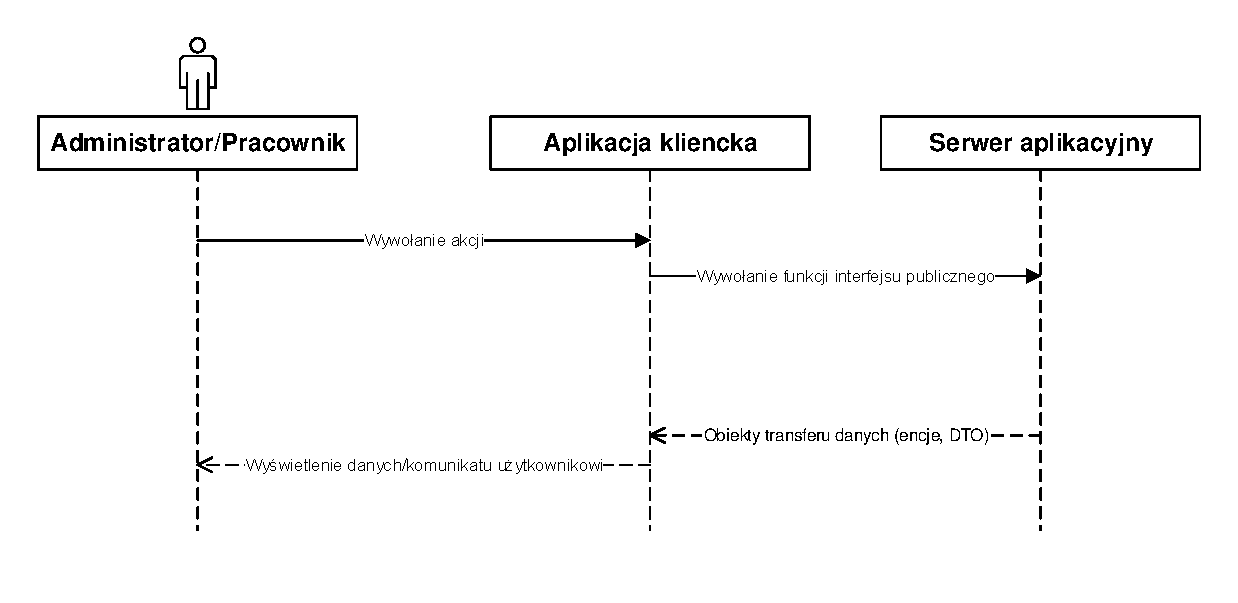
\includegraphics[width=16cm]{Resources/PDF/sequence-client.pdf}
	\caption{Diagram sekwencji -- komunikacja aplikacji klienckiej z serwerem aplikacyjnym}
\end{figure}
\begin{table}[H]
	\begin{tabularx}{\textwidth}{|l|l|X|}
		\hline
		\textbf{Funkcjonalność} & \textbf{System} & \textbf{Opis} \\
		\hline
		Wywołanie akcji &
		Aplikacja kliencka &
		\textbf{Działanie biznesowe:} \\
		& & Administrator lub pracownik wykonują akcję za pośrednictwem interfejsu graficznego aplikacji klienckiej. \\
		& & \textbf{Wejście:} Akcja wykonana w interfejsie graficznym. \\
		& & \textbf{Wyjście:} Wyświetlenie rezultatu akcji -- wyszukiwanych danych lub komunikatu o niepowodzeniu akcji. \\
		\hline
		Wywołanie funkcji interfejsu &
		Obiekty serwisowe &
		\textbf{Działanie biznesowe:} \\
		& & Aplikacja kliencka przesyła dane dotyczące akcji podjętej przez użytkownika do warstwy serwisowej za pomocą jej interfejsu publicznego. \\
		& & \textbf{Wejście:} Dane dotyczące podjętej akcji. \\
		& & \textbf{Wyjście:} Obiekty transferu danych zawierające informacje o rezultacie danej akcji. \\
		\hline
	\end{tabularx}
\end{table}

\subsubsection{Interfejs webowy}
\begin{figure}[H]
	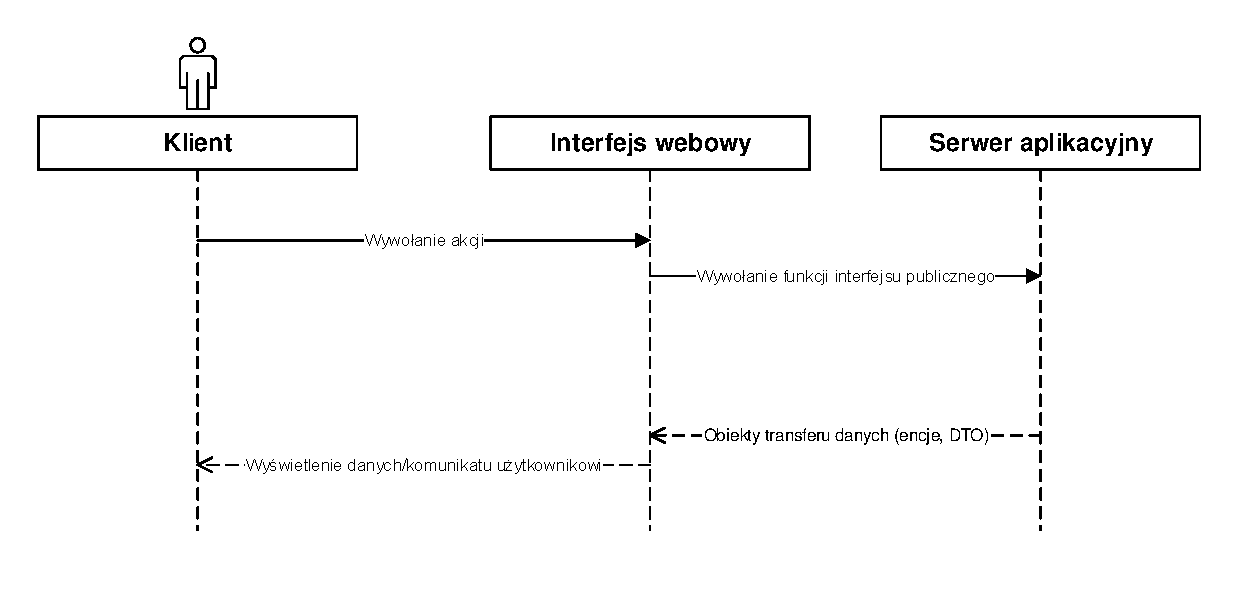
\includegraphics[width=16cm]{Resources/PDF/sequence-web.pdf}
	\caption{Diagram sekwencji -- komunikacja interfejsu webowego z serwerem aplikacyjnym}
\end{figure}
\begin{table}[H]
	\begin{tabularx}{\textwidth}{|l|l|X|}
		\hline
		\textbf{Funkcjonalność} & \textbf{System} & \textbf{Opis} \\
		\hline
		Wywołanie akcji &
		Interfejs webowy &
		\textbf{Działanie biznesowe:} \\
		& & Klient wykonuje akcję za pośrednictwem interfejsu webowego. \\
		& & \textbf{Wejście:} Akcja wykonana w interfejsie webowym. \\
		& & \textbf{Wyjście:} Wyświetlenie rezultatu akcji -- wyszukiwanych danych lub komunikatu o niepowodzeniu akcji. \\
		\hline
		Wywołanie funkcji interfejsu &
		Obiekty serwisowe &
		\textbf{Działanie biznesowe:} \\
		& & Interfejs webowy przesyła dane dotyczące akcji podjętej przez użytkownika do warstwy serwisowej za pomocą jej interfejsu publicznego. \\
		& & \textbf{Wejście:} Dane dotyczące podjętej akcji. \\
		& & \textbf{Wyjście:} Obiekty transferu danych zawierające informacje o rezultacie danej akcji. \\
		\hline
	\end{tabularx}
\end{table}

\subsubsection{Serwer aplikacyjny}
\begin{figure}[H]
	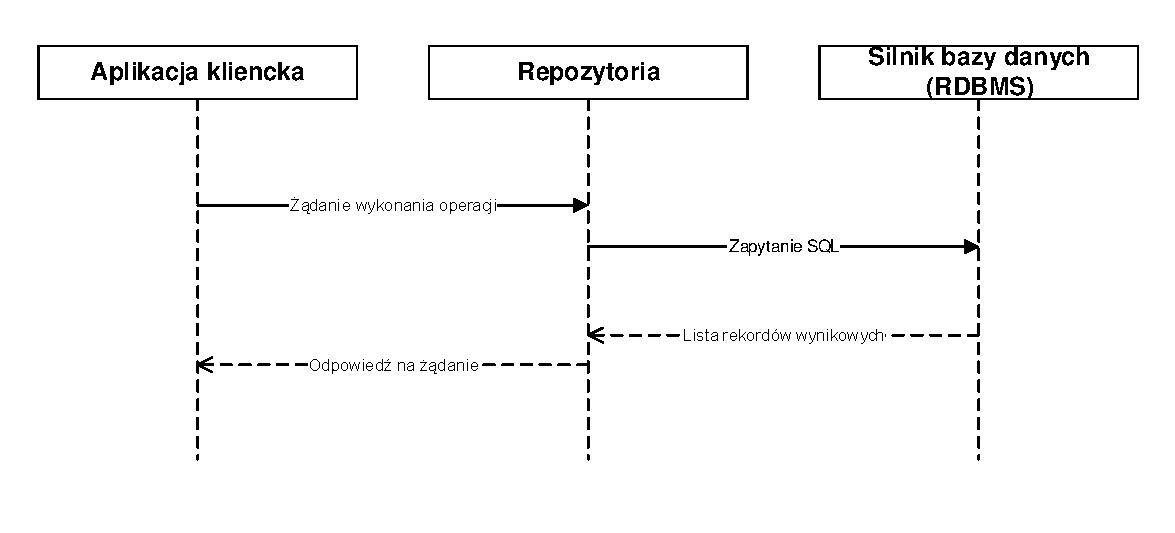
\includegraphics[width=16cm]{Resources/PDF/sequence-server.pdf}
	\caption{Diagram sekwencji -- przepływ danych w obrębie serwera aplikacyjnego}
\end{figure}
\begin{table}[H]
	\begin{tabularx}{\textwidth}{|l|l|X|}
		\hline
		\textbf{Funkcjonalność} & \textbf{System} & \textbf{Opis} \\
		\hline
		Otrzymanie żądania &
		Serwer aplikacyjny &
		\textbf{Działanie biznesowe:} \\
		& & Serwer aplikacyjny otrzymuje żądanie od jednej z aplikacji klienckich lub interfejsu webowego za pośrednictwem protokołu HTTP. \\
		& & \textbf{Wejście:} Żądanie XML SOAP do wykonania. \\
		& & \textbf{Wyjście:} Odpowiedź na żądanie aplikacji klienckiej lub interfejsu webowego. \\
		\hline
		Wywołanie funkcji repozytorium &
		Obiekty serwisowe &
		\textbf{Działanie biznesowe:} \\
		& & Serwer aplikacyjny przetwarza otrzymane wcześniej żądanie i buduje z niego zapytanie SQL. \\
		& & \textbf{Wejście:} Wejściowy obiekt DTO. \\
		& & \textbf{Wyjście:} Wynikowy obiekt DTO lub informacja o błędzie (wyjątek). \\
		\hline
		Zapytanie SQL &
		Silnik bazy danych &
		\textbf{Działanie biznesowe:} \\
		& & Dane odebrane od klienta są przetwarzane na zapytania SQL do bazy danych. \\
		& & \textbf{Wejście:} Zapytanie SQL służące pobraniu lub modyfikacji danych. \\
		& & \textbf{Wyjście:} Rekordy wynikowe pobrane z bazy danych. \\
		\hline
	\end{tabularx}
\end{table}

\newpage
\subsection{Model danych}
Model danych użyty w systemie został przedstawiony w formie diagramu relacji na poniższej grafice:
\begin{figure}[H]
	\centering
	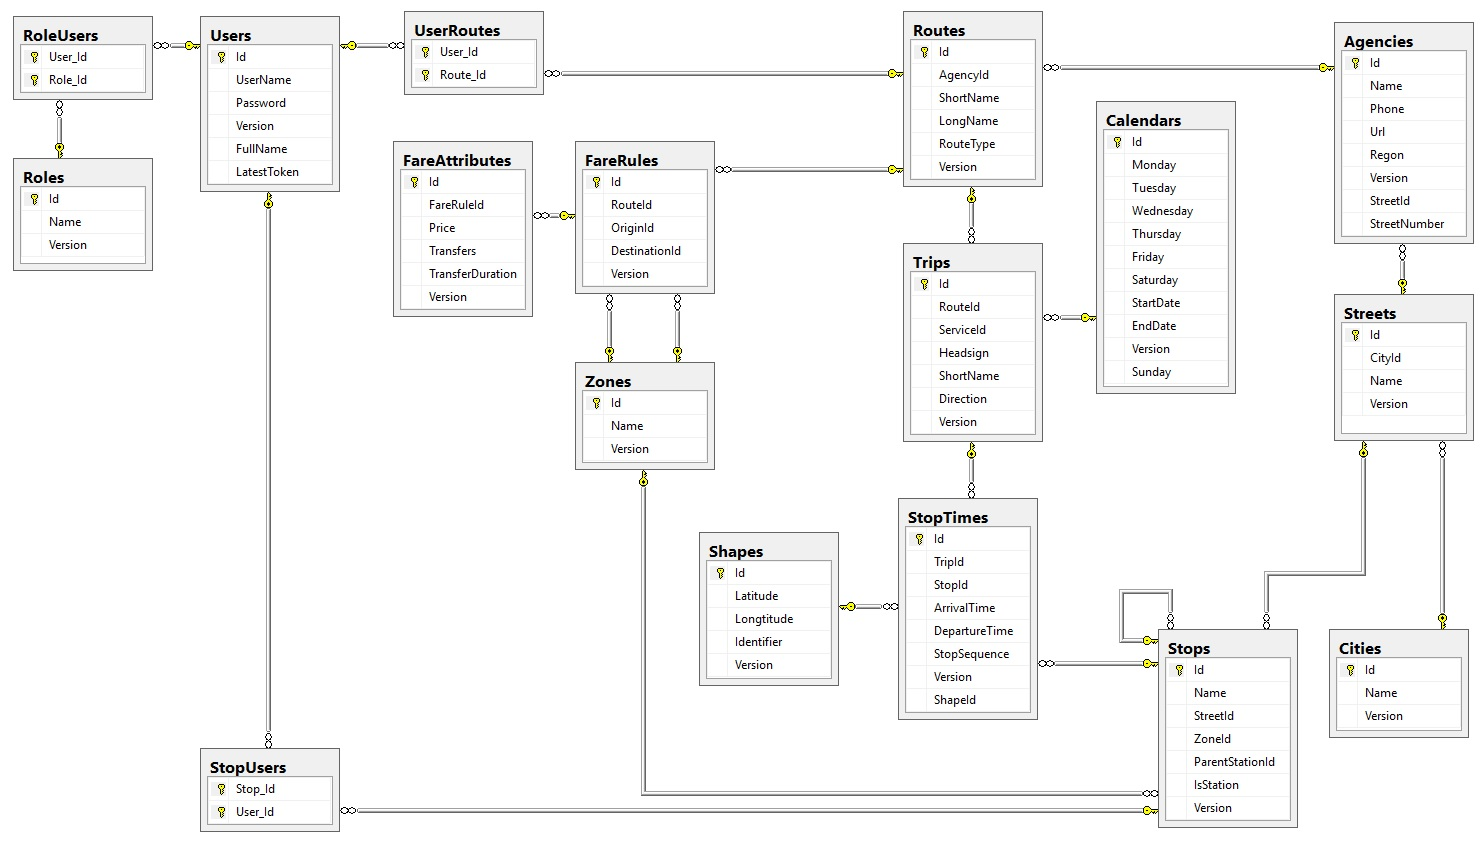
\includegraphics[scale = 0.4]{Resources/Images/data-model.jpg}
	\caption{Diagram relacji}
\end{figure}
Poniżej opisano znaczenie i rodzaj relacji zachodzących pomiędzy encjami w systemie.
\begin{enumerate}
	\item \textbf{User - Role} jest relacją wiele do wielu zrealizowaną przy pomocy tabeli pomocniczej UserRoles. Są to tabele niezależne od reszty systemu, ponieważ służą jedynie zdefiniowaniu elementów aplikacji dostępnych dla danego użytkownika.
	\item \textbf{City - Street} to relacja jeden do wielu. Ulice zdefiniowane w systemie zawierają informację o mieście, w którym są.
	\item Informacje o ulicy (a co za tym idzie również o mieście) zawarte są w poszczególnych agencjach (przewoźnikach) oraz przystankach, stąd relacje jeden do wielu \textbf{Street - Agency} oraz \textbf{Street - Stop}.
	\item Każdy przewoźnik zapewnia wiele połączeń różnymi środkami komunikacji, dlatego relacja \textbf{Agency - Route} jest relacją jeden do wielu.
	\item Poszczególne połączenia są jedynie definicją trasy. Sam przejazd (których może być wiele) pomiędzy punktami trasy zawarty jest w tabeli \textbf{Trips}. Przejazd musi zostać ponadto umieszczony w czasie, stąd dodatkowa tabela \textbf{Calendars}, która mówi w jakich dniach połączenie będzie funkcjonować. Tak określone relacje \textbf{Route - Trip} oraz \textbf{Calendar - Trip} są jeden do wielu.
	\item Należy również określić konkretne czasy postojów na trasie przejazdu. Tym zajmuje się tabela \textbf{StopTimes}, w której zdefiniowane poszczególne postoje są skojarzone z konkretnym przejazdem i przystankiem. To powoduje, że relacje \textbf{Trip - StopTime} oraz \textbf{Stop - StopTime} są jeden do wielu.
	\item Należy równiez zdefiniować strefy przejazdu, czym zajmuje się tabela \textbf{Zones}. Każdy przystanek ma przypisaną konkretną strefę w której się znajduje, więc relacja \textbf{Zone - Stop} jest jeden do wielu.
	\item Każda trasa może mieć inny cennik, a cena biletu może się zmieniać w zależności od początkowej i końcowej strefy. Stąd relacja \textbf{Route - FareAttribute} jest jeden do wielu. Ponadto wiele tras może korzystać z jednego cennika, dlatego relacja \textbf{FareRule - FareAttribute} jest również jeden do wielu.
	\item Z tabelą \textbf{StopTimes} powiązana jest tabela \textbf{Shapes}, która zawiera dane określające położenie geograficzne dla poszczególnych postojów. Dane te wykorzystywane są do generowania map.
	\item Tabele \textbf{UserRoutes} i \textbf{StopUsers} odpowiadają za przechowywanie ulubionych tras i przystanków użytkowników.
\end{enumerate}

\subsection{Scenariusze testów akceptacyjnych i raport z ich przeprowadzenia}

\subsubsection{Aplikacja wewnętrzna}

\begin{tabularx}{\textwidth}{|X|X|X|X|l|}
	\hline
	\textbf{Rola} & \textbf{Testowana funkcjonalność} & \textbf{Opis czynności} & \textbf{Oczekiwany rezultat} & \textbf{Wynik testu} \\
	\hline
	Administrator &
	Dodanie nowego użytkownika &
	Wybranie zakładki \textbf{Users} na bocznym pasku aplikacji, przejście do widoku dodawania użytkownika po wciśnięciu przycisku \textbf{Add New} oraz zapisanie zmian przyciskiem \textbf{Save}. &
	Nowy użytkownik zostanie dodany do bazy danych. &
	Pozytywny \\
	\hline
	Administrator &
	Modyfikacja istniejącego użytkownika &
	Wybranie zakładki \textbf{Users} na bocznym pasku aplikacji, wyszukanie istniejącego użytkownika, przejście do widoku edycji użytkownika po zaznaczeniu jednego z listy i wciśnięciu przycisku \textbf{Edit Selected} oraz zapisanie zmian przyciskiem \textbf{Save}. &
	Dane wybranego użytkownika zostaną zmodyfikowane. &
	Pozytywny \\
	\hline
	Administrator &
	Usunięcie istniejącego użytkownika &
	Wybranie zakładki \textbf{Users} na bocznym pasku aplikacji, wyszukanie istniejącego użytkownika i wciśnięcie przycisku \textbf{Delete Selected} po wybraniu jednego z listy. &
	Dane wybranego użytkownika zostaną usunięte. &
	Pozytywny \\
	\hline
	Administrator &
	Usunięcie istniejącego użytkownika &
	Wybranie zakładki \textbf{Users} na bocznym pasku aplikacji, wyszukanie istniejącego użytkownika i wciśnięcie przycisku \textbf{Delete Selected} po wybraniu jednego z listy. &
	Dane wybranego użytkownika zostaną usunięte. &
	Pozytywny \\
	\hline 
	Użytkownik &
	Zalogowanie się &
	Wpisanie loginu i hasła w odpowiednie pola na ekranie logowania i wciśnięcie przycisku \textbf{Login} &
	Zalogowanie się do systemu w przypadku poprawnych danych, odmowa dostępu w przypadku niepoprawych danych &
	Pozytywny \\
	\hline
	Zalogowany użytkownik &
	Wylogowanie się &
	Wciśniecię przycisku \textbf{Logout} na bocznym pasku aplikacji. &
	Poprawne wylogowanie się z zystemu i przejście do ekranu logowania. &
	Pozytywny \\
	\hline
	Pracownik &
	Dodanie nowego przewoźnika &
	Wybranie zakładki \textbf{Agencies} w bocznym pasku aplikacji, przejście do widoku dodania przewoźnika po wciśnięciu przycisku \textbf{Add New} oraz zapisanie zmian przyciskiem \textbf{Save}. &
	Nowy przewoźnik zostanie dodany do bazy danych. &
	Pozytywny \\
	\hline
	Pracownik &
	Modyfiacja istniejącego przewoźnika &
	Wybranie zakładki \textbf{Agencies} na bocznym pasku aplikacji, wyszukanie istniejącego przewoźnika, przejście do widoku edycji przewoźnika po zaznaczeniu jednego z listy i wciśnięciu przycisku \textbf{Edit Selected} oraz zapisanie zmian przyciskiem \textbf{Save}. &
	Dane wybranego przewoźnika zostaną zmodyfikowane. &
	Pozytywny \\
	\hline
	Pracownik &
	Usunięcie istniejącego przewoźnika &
	Wybranie zakładki \textbf{Agencies} na bocznym pasku aplikacji, wyszukanie istniejącego przewoźnika i wciśnięcie przycisku \textbf{Delete Selected} po wybraniu jednego z listy. &
	Dane wybranego przewoźnika zostaną usunięte. &
	Pozytywny \\
	\hline
	Pracownik &
	Dodanie nowej linii połączeń &
	Wybranie zakładki \textbf{Routes} w bocznym pasku aplikacji, przejście do widoku dodania połączenia po wciśnięciu przycisku \textbf{Add New} oraz zapisanie zmian przyciskiem \textbf{Save}. &
	Nowe połączenie zostanie dodane do bazy danych. &
	Pozytywny \\
	\hline
	Pracownik &
	Modyfikacja istniejącej linii połączeń &
	Wybranie zakładki \textbf{Routes} na bocznym pasku aplikacji, wyszukanie istniejącego połączenia, przejście do widoku edycji połączenia po zaznaczeniu jednego z listy i wciśnięciu przyciskiem \textbf{Edit Selected} oraz zapisanie zmian przyciskiem \textbf{Save}. &
	Dane dotyczące wybranego połączenia zostaną zmodyfikowane. &
	Pozytywny \\
	\hline
	Pracownik &
	Usunięcie istniejącej linii połączeń &
	Wybranie zakładki \textbf{Routes} na bocznym pasku aplikacji, wyszukanie istniejącego połączenia i wciśnięcie przycisku \textbf{Delete Selected} po wybraniu jednego z listy. &
	Dane dotyczące wybranego połączenia zostaną usunięte. &
	Pozytywny \\
	\hline
	Pracownik &
	Wyświetlanie połączeń przewoźnika &
	Wybranie zakładki \textbf{Routes} na bocznym pasku aplikacji i wybranie konkretnego przewoźnika w opcjach filtrowania. &
	Wyświetlona lista połączeń zapewnionych przez wybranego przewoźnika. &
	Pozytywny \\
	\hline
	Pracownik &
	Wyświetlanie rozkładu jazdy dla linii połączeń &
	Wybranie zakładki \textbf{Routes} na bocznym pasku aplikacji, wyszukanie istniejącego połączenia i wciśnięcie przycisku \textbf{View Timetable} po zaznaczeniu jednego z listy. Następnie przełączając się w liście przystanków po lewej możemy przeglądać godziny przyjazdu i odjazdu na ten przystanek dla danej linii. &
	Informacje o godzinach przyjazdu i odjazdu danej linii na konkretne przystanki. &
	Pozytywny \\
	\hline
	Pracownik &
	Wyświetlanie rozkładu jazdy dla przystanku &
	Wybranie zakładki \textbf{Stops} na bocznym pasku aplikacji, wyszukanie istniejącego przystanku i wciśnięcie przycisku \textbf{View Timetable} po zaznaczeniu jednego z listy. Następnie przełączając się w liście połączeń po lewej możemy przeglądać godziny przyjazdu i odjazdu na ten przystanek dla danej linii. &
	Informacje o godzinach przyjazdu i odjazdu poszczególnych linii połączeń na danym przystanku. &
	Pozytywny \\
	\hline
	Pracownik &
	Wyszukiwanie połączeń pomiędzy dwoma przystankami &
	Wybranie zakładki \textbf{Search Routes} na bocznym pasku aplikacji, wybranie dwóch przystanków i wciśnięcie przycisku \textbf{Find Routes}. &
	Linie połączeń, którymi można przejechać pomiędzy podanymi przystankami. &
	Pozytywny \\
	\hline
\end{tabularx}

\subsubsection{Aplikacja webowa}
\begin{tabularx}{\textwidth}{|X|X|X|l|}
	\hline
	\textbf{Testowana funkcjonalność} & \textbf{Opis czynności} & \textbf{Oczekiwany rezultat} & \textbf{Wynik} \\
	\hline
	\multicolumn{4}{|c|}{\textbf{Niezalogowany użytkownik}} \\
	\hline
	Wyszukanie trasy &
	Otwarcie witryny w przeglądarce, wpisanie nazwy i wybranie dwóch przystanków i wciśnięcie przycisku \textbf{Search}. &
	Wyświetlenie na dole strony listy tras kursujących między wybranymi przystankami. &
	Pozytywny \\
	\hline
	Wyświetlenie mapy dla połączenia &
	Otwarcie witryny w przeglądarce, wpisanie nazwy, wybranie dwóch przystanków i wciśnięcie przycisku \textbf{Search} i wciśnięcie przycisku \textbf{Show map} dla jednego z wyników wyszukiwania. &
	Okno dialogowe pokazujące na mapie trasę wybranego połączenia. &
	Pozytywny \\
	\hline
	Wyświetlanie rozkładu dla trasy &
	Wybranie opcji \textbf{Timetable $\rightarrow$ Search by route}, wyszukanie i wybranie trasy oraz przystanku. &
	Pojawienie się listy rozwijanej z przystankami trasy, pojawienie się rozkładu po wybraniu przystanku. &
	Pozytywny \\
	\hline
	Wyświetlanie rozkładu dla trasy &
	Wybranie opcji \textbf{Timetable $\rightarrow$ Search by stop}, wyszukanie i wybranie przystanku oraz trasy. &
	Pojawienie się listy rozwijanej z trasami przejeżdżającymi przez dany przystanek, pojawienie się rozkładu po wybraniu trasy. &
	Pozytywny \\
	\hline
	Rejestracja konta &
	Wybranie opcji \textbf{Register}, wypełnienie formularza, wciśnięcie przycisku \textbf{Register}. &
	Komunikat o pomyślnym utworzeniu konta. &
	Pozytywny \\
	\hline
	Logowanie &
	Wybranie opcji \textbf{Login}, wprowadzenie nazwy użytkownika oraz hasła, wciśnięcie przycisku \textbf{Login}. &
	Komunikat o pomyślnym zalogowaniu do aplikacji. &
	Pozytywny \\
	\hline
	\multicolumn{4}{|c|}{\textbf{Zalogowany użytkownik}} \\
	\hline
	Dodanie, usunięcie ulubionego przystanku &
	Wybranie opcji \textbf{Favourites}, usunięcie jednego oraz dodanie innego przystanku w zakładce \textbf{Stops}, kliknięcie przycisku \textbf{Save changes}. &
	Komunikat o zapisaniu zmian w ulubionych. &
	Pozytywny \\
	\hline
	Dodanie, usunięcie ulubionej trasy &
	Wybranie opcji \textbf{Favourites}, usunięcie jednej oraz dodanie innej trasy w zakładce \textbf{Routes}, kliknięcie przycisku \textbf{Save changes}. &
	Komunikat o zapisaniu zmian w ulubionych. &
	Pozytywny \\
	\hline
	Zmiana hasła &
	Wybranie opcji \textbf{Settings} z menu rozwijanego w prawym górnym rogu etykietowanego nazwą użytkownika, wypełnienie formularza zmiany hasła, wciśnięcie przycisku \textbf{Save changes}, wylogowanie się i zalogowanie z nowym hasłem. &
	Pomyślne zalogowanie się do systemu. &
	Pozytywny \\
	\hline
	Wylogowanie &
	Wybranie opcji \textbf{Logout}  z menu rozwijanego w prawym górnym rogu etykietowanego nazwą użytkownika. &
	Powiadomienie o wylogowaniu się z aplikacja, zniknięcie opcji \textbf{Favourites} i menu rozwijanego z paska nawigacyjnego. &
	Pozytywny \\
	\hline
\end{tabularx}

\begin{comment}
\subsection{Raport z przeprowadzonych testów}
\end{comment}

\newpage
\section{Lista użytych skrótów}
\label{abbr:bsd}
\paragraph{BSD} Berkeley Software Distribution

\label{abbr:ioc}
\paragraph{IoC} Inversion of Control

\label{abbr:mit}
\paragraph{MIT} Massachussetts Institute of Technology  

\label{abbr:mspl}
\paragraph{MS-PL} Microsoft Software Public License

\label{abbr:mvvm}
\paragraph{MVVM} \textbf{ang.} Model-View-ViewModel -- wzorzec używany w projektach realizowanych w technologii \hyperref[abbr:wpf]{WPF} pozwalający na odseparowanie logiki aplikacji od warstwy prezentacyjnej. 

\label{abbr:wpf}
\paragraph{WPF} Windows Presentation Framework

\renewcommand*{\refname}{\vspace*{-2em}}
\section{Bibliografia}
\begin{thebibliography}{99}

\bibitem{castlecore}
	Castle Project,
	\emph{Castle Core},
	\url{https://github.com/castleproject/Core}

\bibitem{entityframework}
	ASP.NET,
	\emph{Entity Framework 6},
	\url{https://github.com/aspnet/EntityFramework6}

\bibitem{fluentassertions}
	Dennis Doomen,
	\emph{FluentAssertions},
	\url{https://github.com/dennisdoomen/fluentassertions}

\bibitem{moq}
	Moq,
	\emph{Moq 4},
	\url{https://github.com/moq/moq4}

\bibitem{nunit}
	NUnit,
	\emph{NUnit},
	\url{https://github.com/nunit/nunit}

\bibitem{reactiveui}
	ReactiveUI,
	\emph{ReactiveUI},
	\url{https://github.com/reactiveui/ReactiveUI}

\bibitem{reactiveextensions}
	Reactive Extensions,
	\emph{Rx.NET},
	\url{https://github.com/Reactive-Extensions/Rx.NET}

\bibitem{splat}
	Paul Betts,
	\emph{Splat},
	\url{https://github.com/paulcbetts/splat}

\bibitem{mahapps}
	MahApps,
	\emph{Metro},
	\url{https://mahapps.com}

\bibitem{angularjs}
	AngularJS,
	Google,
	\url{https://angularjs.org/}.

\bibitem{angularspinner}
	angular-spinner,
	Uri Shaked,
	\url{https://github.com/urish/angular-spinner}.

\bibitem{spinjs}
	spin.js,
	Felix Gnass,
	\url{http://spin.js.org/}.

\bibitem{toastr}
	angular-toastr,
	Jesús Rodríguez,
	\url{https://github.com/Foxandxss/angular-toastr}.

\bibitem{angularevent}
	angular-event-aggregator,
	Vladimir Gurovich,
	\url{https://github.com/vladgurovich/angular-event-aggregator}.

\bibitem{uirouter}
	Angular UI Router,
	Angular UI Team,
	\url{https://github.com/angular-ui/ui-router}.

\bibitem{uibootstrap}
	Angular UI Bootstrap,
	Angular UI Team,
	\url{https://github.com/angular-ui/bootstrap}.

\bibitem{fontawesome}
	Font Awesome,
	Angular UI Team,
	\url{http://fontawesome.io/}.

\bibitem{bootstrap}
	Bootstrap,
	Dave Gandy,
	\url{http://getbootstrap.com}.

\bibitem{oauth}
	OAuth 2.0,
	OWIN,
	\url{https://www.asp.net/aspnet/overview/owin-and-katana/owin-oauth-20-authorization-server}.

\bibitem{unity}
	Unity,
	Microsoft,
	\url{https://msdn.microsoft.com/en-us/library/dn507457(v=pandp.30).aspx}.

\bibitem{ngmap}
	AngularJS Google Maps,
	Allen Kim,
	\url{https://github.com/allenhwkim/angularjs-google-maps}.

\bibitem{jquery}
	jQuery,
 	The jQuery Foundation,
	\url{http://jquery.com/}.

\bibitem{sqlserver}
	Installing SQL Server 2014 Step By Step Tutorial,
	Microsoft TechNet,
	\url{http://social.technet.microsoft.com/wiki/contents/articles/23878.installing-sql-server-2014-step-by-step-tutorial.aspx}.

\bibitem{iis}
	Installing IIS 8 on Windows Server 2012,
	Microsoft,
	\url{https://www.iis.net/learn/get-started/whats-new-in-iis-8/installing-iis-8-on-windows-server-2012}.

\bibitem{aspnet}
	IIS 8.0 ASP.NET Configuration Management,
	Microsoft,
	\url{https://www.iis.net/learn/get-started/whats-new-in-iis-8/iis-80-aspnet-configuration-management}.

\end{thebibliography}
\end{document}
